\chapter{First-Order Logic}
In \textcolor{blue}{propositional logic}, we have studied the combination of atomic propositions using
the propositional \textcolor{blue}{connectives} ``$\neg$'', ``$\vee$'', ``$\wedge$'', ``$\rightarrow$" and
``$\leftrightarrow$''.  In \blue{first-order logic}\index{first-order logic} we additionally 
examine the structure of these atomic propositions. The following additional concepts are introduced in
first-order logic: 
\begin{enumerate}
\item \textcolor{blue}{Terms} are used as designations for objects.
\item These terms are composed of \textcolor{blue}{object variables} and \textcolor{blue}{function symbols}.
      In the following examples, ``$x$'' is an object variable\index{Object variable}, while
      ``\textsl{father}'' and ``\textsl{mother}'' are unary function symbols\index{function symbol} and
      ``\textsl{isaac}'' is a nullary function symbol:
      \\[0.2cm]
      \hspace*{1.3cm}
      $\textsl{father}(x),\quad \textsl{mother}(\textsl{isaac})$.
      \\[0.2cm]
      Nullary function symbols are also referred to as \textcolor{blue}{constants}\index{constant}
      and instead of object variables we simply talk about variables.
\item Different objects are related by \textcolor{blue}{predicate symbols}\index{Predicate symbols}.
      In the following example, we use the predicate symbols ``\textsl{isBrother}'' and ``$<$''.
      Additionally, ``\textsl{albert}'' and ``\textsl{bruno}'' are constants:
      \\[0.2cm]
      \hspace*{1.3cm}
      $\textsl{isBrother}\bigl(\textsl{albert}, \textsl{father}(\textsl{bruno})\bigr),\quad x+7 < x\cdot 7$.
      \\[0.2cm]
      The resulting formulas are referred to as \textcolor{blue}{atomic formulas} \index{atomic formulas},
      since they do not contain subformulas. 
\item Atomic formulas can be combined using the propositional connectives as shown the following example:
      \\[0.2cm]
      \hspace*{1.3cm}
      $x > 1 \rightarrow x + 7 < x \cdot  7$.
\item Finally, the \textcolor{blue}{quantifiers}\index{quantifiers} ``$\forall$'' (\emph{for all}) and
      ``$\exists$'' (\emph{there exists}) are introduced to distinguish between variables that are
      \textcolor{blue}{existentially} quantified and those variables that are \textcolor{blue}{universally}
      quantified.  For example, the formula 
      \\[0.2cm]
      \hspace*{1.3cm}
      $\forall x \in \mathbb{R}: \exists n \in \mathbb{N}: x < n$
      \\[0.2cm]
      is read as: ``\textsl{For all real numbers $x$ there exists a natural number $n$ such that $x$ is less
        than $n$.}''
\end{enumerate}
This chapter is structured as follows:
\begin{enumerate}[(a)]
\item In the next section, we will define the \href{https://en.wikipedia.org/wiki/Syntax}{syntax} of
      first-order logic formulas, i.e., we will specify those strings that are regarded as first-order
      formulas.
\item In the following section, we deal with the
      \href{https://en.wikipedia.org/wiki/Semantics}{semantics} of these formulas, that is we specify the 
      meaning of first-order formulas.
\item After that, we show how to implement syntax and semantics in \textsl{Python}.
\item As an application of first-order logic we discuss \textcolor{blue}{constraint programming}.
      In constraint programming, a given problem is described using first-order logic formulas.
      To solve the problem, a so-called \textcolor{blue}{constraint solver} is used.
\item We develop a simple constraint solver that works by the means of \blue{backtracking}.
\item Then we discuss the constraint solver \texttt{Z3}, which is a state-of-the-art constraint solver
      developed by Microsoft Corporation.
\item Furthermore, we consider normal forms of first-order logic formulas and show how formulas
      can be transformed into first-order logic clauses.
\item We also discuss a \textcolor{blue}{first-order logic calculus}, which is the basis
      of automatic reasoning in first-order logic.
\item To conclude the chapter, we discuss the automatic theorem prover \textsl{Vampire}.
\end{enumerate}

\section{Syntax of First-Order Logic}
First, we define the concept of a \textcolor{blue}{signature}\index{signature}. Essentially, this is a
structured summary of variables, function symbols, and predicate symbols, along with a specification of the
arity of these symbols. 

\begin{Definition}[Signature]
  A \textcolor{blue}{signature} is a 4-tuple \\[0.2cm]
  \hspace*{1.3cm} $\Sigma = \langle \mathcal{V}, \mathcal{F}, \mathcal{P}, \textsl{arity} \rangle$, \\[0.2cm]
  such that the following holds:
  \begin{enumerate}
  \item $\mathcal{V}$ is the set of \textcolor{blue}{object variables},\index{Object variables} which we often simply refer to as
        \textcolor{blue}{variables} for brevity.
  \item $\mathcal{F}$ is the set of \textcolor{blue}{function symbols}.\index{Function symbols}
  \item $\mathcal{P}$ is the set of \textcolor{blue}{predicate symbols}.\index{Predicate symbols}
  \item $\textsl{arity}$ is a function that assigns each function and predicate symbol its
        \textcolor{blue}{arity}\index{Arity}: \\[0.2cm]
        \hspace*{1.3cm} $\textsl{arity}: \mathcal{F} \cup \mathcal{P} \rightarrow \mathbb{N}$. \\[0.2cm]
        We say that the function or predicate symbol $f$ is an
        $n$-ary symbol if $\textsl{arity}(f) = n$.
        
        A function symbol $c$ such that $\textsl{arity}(c) = 0$ is called a \blue{constant}. \index{constant}
        
        A predicate symbol $p$ such that $\textsl{arity}(p) = 0$ is called a \blue{propositional variable}.
        \index{propositional variable}
  \item Since we need to be able to distinguish between variables, function symbols, and predicate symbols,
        we agree that the sets $\mathcal{V}$, $\mathcal{F}$, and $\mathcal{P}$ have to be pairwise disjoint: \\[0.2cm] 
        \hspace*{1.3cm} $\mathcal{V} \cap \mathcal{F} = \{\}$, \quad
                        $\mathcal{V} \cap \mathcal{P} = \{\}$, \quad and \quad
                        $\mathcal{F} \cap \mathcal{P} = \{\}$. \eox
  \end{enumerate}
\end{Definition}

\exampleEng
Next, we define the signature $\Sigma_G$ of group theory. Let
\begin{enumerate}
\item $\mathcal{V} := \{ x, y, z \}$ be the set of variables,
\item $\mathcal{F} := \{ \mathtt{e}, \circ \}$ be the set of function symbols,
\item $\mathcal{P} := \{\mathtt{=} \}$ be the set of predicate symbols,
\item $\textsl{arity} := \bigl\{ \mathtt{e} \mapsto 0, \mathtt{\circ} \mapsto 2, = \mapsto 2 \bigr\}$
      specifes the arities of function and predicate symbols.
\end{enumerate}
Then the signature $\Sigma_G$ of group theory is defined as follows:
\\[0.2cm]
\hspace*{1.3cm}
$\Sigma_G := \langle \mathcal{V}, \mathcal{F}, \mathcal{P}, \textsl{arity} \rangle$.
\eox
\vspace{0.3cm}

\noindent
We use expressions built from variables and function symbols as identifiers for objects. These expressions are
called \textcolor{blue}{terms}.\index{terms} The formal definition follows.

\begin{Definition}[Terms, $\mathcal{T}_\Sigma$] \hspace*{\fill} \\
  If $\Sigma = \langle \mathcal{V}, \mathcal{F}, \mathcal{P}, \textsl{arity} \rangle$ is a signature, then we
  define the set \textcolor{blue}{$\mathcal{T}_\Sigma$} \index{$\mathcal{T}_\Sigma$}  of
  \textcolor{blue}{$\Sigma$-terms}, 
  inductively:
  \begin{enumerate}
  \item For every variable $x \in \mathcal{V}$, we have that $x \in \mathcal{T}_\Sigma$. Thus, every variable is also a term.
  \item If $c \in \mathcal{F}$ is a $0$-ary function symbol,
        i.e.~$\textsl{arity}(c) = 0$, then $c \in \mathcal{T}_\Sigma$.

        Therefore, every constant is a term.
  \item If $f \in \mathcal{F}$ is an $n$-ary function symbol such that $n > 0$ and 
        $t_1,\cdots,t_n \in \mathcal{T}_\Sigma$, then 
        \\[0.2cm]
        \hspace*{1.3cm} $f(t_1,\cdots,t_n) \in \mathcal{T}_\Sigma$,
        \\[0.2cm]
        thus the expression $f(t_1,\cdots,t_n) \in \mathcal{T}_\Sigma$ is a term.
        \eox
  \end{enumerate}
\end{Definition}

\exampleEng
Let
\begin{enumerate}
\item $\mathcal{V} := \{ x, y, z \}$ be the set of variables,
\item $\mathcal{F} := \{ 0, 1, \mathtt{+}, \mathtt{-}, * \}$ be the set of function symbols,
\item $\mathcal{P} := \{\mathtt{=}, \leq\}$ be the set of predicate symbols,
\item $\textsl{arity} := \bigl\{ 0 \mapsto 0, 1 \mapsto 0, \mathtt{+} \mapsto 2, \mathtt{-} \mapsto 2,
                                 * \mapsto 2, = \mapsto 2, \leq \mapsto 2 \bigr\}$
      specify the arity of function and predicate symbols, and
\item $\Sigma_\mathrm{arith} := \langle \mathcal{V}, \mathcal{F}, \mathcal{P}, \textsl{arity} \rangle$
      be a signature.
\end{enumerate}
Then we can construct $\Sigma_{\mathrm{arith}}$-terms as follows:
\begin{enumerate}
\item $x, y, z \in \mathcal{T}_{\Sigma_{\mathrm{arith}}}$, \\[0.2cm]
      since all variables are also $\Sigma_{\mathrm{arith}}$-terms.
\item $0, 1 \in \mathcal{T}_{\Sigma_{\mathrm{arith}}}$,  \\[0.2cm]
      since $0$ and $1$ are nullary function symbols.
\item $\mathtt{+}(0,x) \in \mathcal{T}_{\Sigma_{\mathrm{arith}}}$, \\[0.2cm]
      since $0 \in \mathcal{T}_{\Sigma_{\mathrm{arith}}}$, $x \in \mathcal{T}_{\Sigma_{\mathrm{arith}}}$ and 
      $\mathtt{+}$ is a binary function symbol.
\item $*(\mathtt{+}(0,x),1) \in \mathcal{T}_{\Sigma_{\mathrm{arith}}}$, \\[0.2cm]
      since $\mathtt{+}(0,x) \in \mathcal{T}_{\Sigma_{\mathrm{arith}}}$, $1 \in \mathcal{T}_{\Sigma_{\mathrm{arith}}}$ and
      $*$ is a binary function symbol.
\end{enumerate}
In practice, for certain binary functions, we use an \textcolor{blue}{infix notation},
i.e., we write binary function symbols between their arguments. For example,
we write $x+y$ instead of $+(x,y)$. The infix notation is then to be understood as an abbreviation for the
above-defined representation. This, of course, works only if we also set precedence levels for the various operators.
\eox

Next, we define the concept of \textcolor{blue}{atomic formulas}.\index{Atomic Formulas} These are formulas
that cannot be decomposed into smaller formulas: atomic formulas thus contain neither propositional connectives
nor quantifiers. 
\begin{Definition}[Atomic Formulas, $\mathcal{A}_\Sigma$]
  Given a signature $\Sigma = \langle \mathcal{V}, \mathcal{F}, \mathcal{P}, \textsl{arity} \rangle$. 
  The set of atomic $\Sigma$-formulas $\mathcal{A}_\Sigma$ \index{$\mathcal{A}_\Sigma$}
  is defined as follows:
  \begin{enumerate}
  \item $\verum \in \mathcal{A}_\Sigma$ and  $\falsum \in \mathcal{A}_\Sigma$.
  \item If $p \in \mathcal{P}$ and $\textsl{arity}(p)= 0$, then $p \in \mathcal{A}_\Sigma$.

        Therefore, propositional variables are atomic formulas.
  \item If $p \in \mathcal{P}$ is an $n$-ary predicate symbol such that $n > 0$ and, furthermore,  $n$ $\Sigma$-terms
        $t_1$, $\cdots$, $t_n$ are given, then  $p(t_1,\cdots,t_n)$ is an \textcolor{blue}{atomic $\Sigma$-formula}: \\[0.2cm]
        \hspace*{1.3cm} $p(t_1,\cdots,t_n) \in \mathcal{A}_\Sigma$.  \qed
  \end{enumerate}
\end{Definition}

\exampleEng
Continuing from the last example, we can see that \\[0.2cm]
\hspace*{1.3cm} $\mathtt{=}(*(\mathtt{+}(0,x),1),0)$ \\[0.2cm]
is an atomic $\Sigma_\mathrm{arith}$-formula. Note that we have not yet discussed the truth value of such
formulas. The question of whether a formula is considered true or false
will be explored in the next section.

In practice we will often use infix notation for binary predicate symbols.  The atomic formula given above is then
written as
\\[0.2cm]
\hspace*{1.3cm}
$(0 + x) * 1 = 0$.
\eox


\subsection{Bound Variables and Free Variables}
In defining first-order logic formulas, it is necessary
to distinguish between so-called \textcolor{blue}{bound}\index{bound variable} and \textcolor{blue}{free}
variables\index{free variable}.
We introduce these concepts informally using an example from calculus.
Consider the following equation: \\[0.2cm]
\hspace*{1.3cm}
$\ds\int_{0}^{x} y \cdot t\, dt = \frac{1}{2} \cdot x^2 \cdot y$
\\[0.2cm]
In this equation, the variables $x$ and $y$ occur \textcolor{blue}{free}, while the variable $t$ is \textcolor{blue}{bound} by the integral.
This means the following: We can substitute arbitrary values for $x$ and $y$ in this equation without
changing the validity of the formula. For example, substituting $2$ for $x$, we get \\[0.2cm]
\hspace*{1.3cm}
$\ds\int_{0}^{2} y \cdot t\, dt = \frac{1}{2} \cdot 2^2 \cdot y$ \\[0.2cm]
and this equation is also valid. Conversely, it makes no sense to substitute a number for the bound variable
$t$.
The left side of the resulting equation would simply be undefined. We can only replace $t$
with another variable.
For example, replacing variable $t$ with $u$, we get \\[0.2cm]
\hspace*{1.3cm}
$\ds\int_{0}^{x} y \cdot u\, du = \frac{1}{2} \cdot x^2 \cdot y$
\\[0.2cm]
and this is effectively the same statement as above. However, this does not work with every variable. If we
substitute the variable $y$ for $t$, we get \\[0.2cm]
\hspace*{1.3cm}
$\ds\int_{0}^{x} y \cdot y\, dy = \frac{1}{2} \cdot x^2 \cdot y$. \\[0.2cm]
This statement is incorrect! The problem is that the previously free variable
$y$ becomes bound during the substitution.

A similar problem arises when we substitute arbitrary terms for $y$. As long as these terms do not contain the variable $t$,
everything is fine. For example, if we substitute the term $x^2$ for $y$, we get \\[0.2cm]
\hspace*{1.3cm}
$\ds\int_{0}^{x} x^2 \cdot t\, dt = \frac{1}{2} \cdot x^2 \cdot x^2$
\\[0.2cm]
and this formula is valid. However, if we substitute the term $t^2$ for $y$, we get \\[0.2cm]
\hspace*{1.3cm}
$\ds\int_{0}^{x} t^2 \cdot t\, dt = \frac{1}{2} \cdot x^2 \cdot t^2$
\\[0.2cm]
and this formula is no longer valid.  These examples show that we have to distinguish between bound and free
variables. 

In first-order logic, the quantifiers ``$\forall$'' (\textcolor{blue}{for all}) and ``$\exists$''
(\textcolor{blue}{there exists}) bind variables in a similar way as the integral operator
``$\int \cdot\; \mathtt{d}t$''. The above explanations show that there are two different types of 
variables: \textcolor{blue}{free variables} and \textcolor{blue}{bound variables}.
To clarify these concepts, we first define for a
$\Sigma$-term $t$ the set of variables contained in $t$.

\begin{Definition}[$\var(t)$]
  \index{$\var(t)$}
  Given a signature $\Sigma = \langle \mathcal{V}, \mathcal{F}, \mathcal{P}, \textsl{arity} \rangle$ and
  $t$ a $\Sigma$-term, we define the set \textcolor{blue}{$\var(t)$} of variables that occur in $t$
  by induction on the structure of the term:
  \begin{enumerate}
    \item $\var(x) := \{ x \}$ \quad for all $x \in \mathcal{V}$,
    \item $\var(c) := \{ \}$ \quad for all $c \in \mathcal{F}$ such that $\textsl{arity}(c) = 0$,
    \item $\var\bigl(f(t_1,\cdots,t_n)\bigr) := \var(t_1) \cup \cdots \cup \var(t_n)$.
          \eox
  \end{enumerate}
\end{Definition}

\subsection{$\Sigma$-Formulas}
\begin{Definition}[$\Sigma$-Formula, $\mathbb{F}_\Sigma$, bound and free variables, $\textsl{BV}(F)$, $\textsl{FV}(F)$]
\label{predicate-formula} \hspace*{\fill}
\index{$\Sigma$-Formula} \index{$\mathbb{F}_\Sigma$}\index{bound variables}\index{free
  variables}\index{$\textsl{BV}(F)$}\index{$\textsl{FV}(F)$} \\
Let $\Sigma = \langle \mathcal{V}, \mathcal{F}, \mathcal{P}, \textsl{arity} \rangle$ be a signature.
    We denote the set of \textcolor{blue}{$\Sigma$-\emph{Formulas}} by $\mathbb{F}_\Sigma$.
    We define this set inductively.
    Simultaneously, for each formula $F \in \mathbb{F}_\Sigma$, we define the set $\textsl{BV}(F)$ of variables
    that occur \textcolor{blue}{bound} in $F$ and the set $\textsl{FV}(F)$ of variables that occur
    \textcolor{blue}{free} in $F$. 
    \begin{enumerate}
    \item $\falsum \in \mathbb{F}_\Sigma$ and $\verum \in \mathbb{F}_\Sigma$, and we define \\[0.2cm]
          \hspace*{1.3cm} $\FV(\falsum) := \FV(\verum) := \BV(\falsum) := \BV(\verum) := \{\}$.
    \item If $p \in \mathcal{A}_\Sigma$ and $\textsl{arity}(p)= 0$, then $p \in \mathbb{F}_\Sigma$ and    
          \\[0.2cm]
          \hspace*{1.3cm}
          \hspace*{1.3cm} $\FV(p) := \{\}$ \quad and \quad $\BV(p) := \{\}$.
    \item If $F = p(t_1,\cdots,t_n)$ is an atomic $\Sigma$-formula, then $F \in \mathbb{F}_\Sigma$.
          Furthermore, we have
          \begin{enumerate}
          \item $\FV\bigl(p(t_1,\cdots,t_n) \bigr) := \var(t_1) \cup \cdots \cup \var(t_n)$,
          \item $\BV\bigl(p(t_1,\cdots,t_n) \bigr) := \{\}$.
          \end{enumerate}
    \item If $F \in \mathbb{F}_\Sigma$, then $\neg F \in \mathbb{F}_\Sigma$.  Furthermore, we have
          \begin{enumerate}
          \item $\FV\bigl( \neg F \bigr) := \FV(F)$,
          \item $\BV\bigl( \neg F \bigr) := \BV(F)$.
          \end{enumerate}
    \item If $F, G \in \mathbb{F}_\Sigma$ and additionally \\[0.2cm]
          \hspace*{1.3cm}
          $\bigl(\FV(F) \cup \FV(G)\bigr) \cap \bigl(\BV(F) \cup \BV(G)) = \{\}$,
          \\[0.2cm]
          then it also holds that
          \begin{enumerate}
          \item $(F \wedge G) \in \mathbb{F}_\Sigma$,
          \item $(F \vee G) \in \mathbb{F}_\Sigma$,
          \item $(F \rightarrow G) \in \mathbb{F}_\Sigma$,
          \item $(F \leftrightarrow G) \in \mathbb{F}_\Sigma$.
          \end{enumerate}
          Furthermore, we define for all propositional connectives $\odot \in \{ \wedge, \vee, \rightarrow, \leftrightarrow \}$:
          \begin{enumerate}
          \item $\FV\bigl((F \odot G) \bigr) := \FV(F) \cup \FV(G)$.
          \item $\BV\bigl((F \odot G) \bigr) := \BV(F) \cup \BV(G)$.
          \end{enumerate}
    \item Let $x \in \mathcal{V}$ and $F \in \mathbb{F}_\Sigma$ with $x \not\in \BV(F)$. Then:
          \begin{enumerate}
          \item $(\forall x : F) \in \mathbb{F}_\Sigma$,
          \item $(\exists x : F) \in \mathbb{F}_\Sigma$.
          \end{enumerate}
          Furthermore, we define
          \begin{enumerate}
          \item $\FV\bigl( (\forall x : F) \bigr) := \FV\bigl( (\exists x : F) \bigr) := \FV(F) \backslash \{x\}$,
          \item $\BV\bigl( (\forall x : F) \bigr) := \BV\bigl( (\exists x : F) \bigr) := \BV(F) \cup \{x\}$.  
          \end{enumerate}
    \end{enumerate}
    If the signature $\Sigma$ is clear from the context or irrelevant, we may also write
    $\mathbb{F}$ instead of $\mathbb{F}_\Sigma$ and simply refer to formulas instead of $\Sigma$-formulas.
    \eox
\end{Definition}

In the definition given above, we have taken care that a variable cannot appear both free and bound in a
formula simultaneously, because a straightforward induction on the structure of the formulas shows that for all 
$F \in \mathbb{F}_\Sigma$ the following holds:  
\\[0.2cm]
\hspace*{1.3cm}
$ \FV(F) \cap \BV(F) = \{\}$. 

\exampleEng
Continuing the example started above, we see that \\[0.2cm]
\hspace*{1.3cm} $(\exists x \colon\, \leq\!(\mathtt{+}(y, x),y))$ \\[0.2cm]
is a formula from $\mathbb{F}_{\Sigma_{\mathrm{arith}}}$. 
The set of bound variables is $\{x\}$, the set of free variables is 
$\{ y \}$. \eox

If we would always write formulas in the prefix notation defined above, then readability would suffer
disproportionately.  
To abbreviate, we agree that in first-order logic the same rules for saving parentheses apply that we have
already used in propositional logic. In addition, the same quantifiers are combined: for example, we write   
\\[0.2cm]
\hspace*{1.3cm}
$\forall x, y \colon p(x, y)  \quad \text{instead of} \quad \forall x \colon ( \forall y \colon p(x,y))$.
\\[0.2cm]
Moreover, we agree that we may also indicate binary predicate and function symbols in infix notation.
In order to guarantee a unique readability, we must then define the precedence and the associativity of the
function symbols.  For example, we write \\[0.2cm]
\hspace*{1.3cm} $\mathtt{n}_1 = \mathtt{n}_2$  \quad instead of \quad $=(\mathtt{n}_1, \mathtt{n}_2)$. \\[0.2cm]
The formula $(\exists x \colon \leq(\mathtt{+}(y, x),y))$ becomes more readable as \\[0.2cm]
\hspace*{1.3cm} $\exists x \colon y + x \leq y$ \\[0.2cm]
Moreover, in the literature, you will often find expressions of the form
\\[0.2cm]
\hspace*{1.3cm}
$\forall x \in M: F$ \quad or \quad $\exists x \in M: F$.
\\[0.2cm]
These are abbreviations defined as
\\[0.2cm]
\hspace*{1.3cm}
$\ds \bigl(\forall x \in M: F\bigr) \stackrel{\mathrm{def}}{\Longleftrightarrow} \forall x: \bigl(x \in M \rightarrow F\bigr)$
\quad and \quad 
$\ds\bigl(\exists x \in M: F\bigr) \stackrel{\mathrm{def}}{\Longleftrightarrow} \exists x: \bigl(x \in M \wedge F\bigr)$.
\\[0.2cm]
Finally, we agree that quantifiers bind more tightly than the operators $\wedge$, $\vee$, $\rightarrow$, and
$\leftrightarrow$. 

\exerciseEng
\noindent \textbf{Consider the following signature for formalizing family relationships:}
\begin{itemize}
    \item \textbf{Variables:} $\{ u, v, w, x, y, z \}$.
    \item \textbf{Function Symbols:}
    \begin{itemize}
        \item $\texttt{mother}(x)$: the mother of $x$.
        \item $\texttt{father}(x)$: the father of $x$.
    \end{itemize}
    \item \textbf{Unary Predicates:}
    \begin{itemize}
        \item $\texttt{female}(x)$: $x$ is female.
        \item $\texttt{male}(x)$: $x$ is male.
    \end{itemize}
    \item \textbf{Binary Predicates:}
    \begin{itemize}
    \item $\texttt{brother}(x,y)$: $x$ is a brother of $y$.
    \item $\texttt{sister}(x,y)$: $x$ is a sister of $y$.
    \item $\texttt{sibling}(x,y)$: $x$ is a sibling of $y$.
    \item $\texttt{married}(x,y)$: $x$ is married to $y$.
    \item $\texttt{grandmother}(x,y)$: $x$ is a grandmother of $y$.
    \item $\texttt{grandfather}(x,y)$: $x$ is a grandfather of $y$.
    \item $\texttt{grandchild}(x, y)$: $x$ is a grandchild of $y$,
    \item $\texttt{uncle}(x,y)$: $x$ is an uncle of $y$.
    \item $\texttt{aunt}(x,y)$: $x$ is an aunt of $y$.
    \item $\texttt{cousin}(x,y)$: $x$ is a cousin of $y$.
    \end{itemize}
\end{itemize}
In the following, your task is to \blue{define} certain predicates. In general, a \blue{definition} of an
$n$-ary predicate $p$ has the form 
\\[0.2cm]
\hspace*{1.3cm}
$\forall x_1, \cdots, x_n: \bigl(p(x_1,\cdots,x_n) \leftrightarrow F\bigr)$,
\\[0.2cm]
where $F$ is a formula that does not contain the predicate $p$.  In this exercise, this formula
may only contain the function symbols \texttt{mother} and \texttt{father} and the predicate symbols \texttt{male} and
\texttt{female}.  For the purpose of this exercise we make the simplifying assumption that
every person is either femal or male.

As an example, to \texttt{define} the predicate \texttt{brother} we can use the following formula:
\\[0.2cm]
\hspace*{1.3cm}
$\forall x, y:\bigl(\mathtt{brother}(x, y) \leftrightarrow \mathtt{male}(x) \wedge \mathtt{father}(x)
= \mathtt{father}(y) \wedge \mathtt{mother}(x) = \mathtt{mother}(y)\bigr)$
\\[0.2cm]
Define the following predicates:
\begin{enumerate}[(a)]
\item $\texttt{sister}(x, y)$,
\item $\texttt{aunt}(x, y)$,
\item $\mathtt{uncle}$,
\item $\texttt{sibling}(x, y)$,
\item $\texttt{grandfather}(x, y)$,
\item $\texttt{grandmother}(x, y)$,
\item $\texttt{grandchild}(x, y)$,
\item $\texttt{cousin}(x, y)$.
  \eox
\end{enumerate}


\section{Semantics of First-Order Logic \label{sec:semantik}}
Next, we define the \blue{meaning} of the formulas. For this purpose, we introduce the concept of a
\blue{$\Sigma$-structure}. \index{$\Sigma$-structure} This kind of structure specifies how the
function and predicate symbols of the signature $\Sigma$ are to be interpreted.

\begin{Definition}[Structure]
    Let a signature \\[0.2cm]
    \hspace*{1.3cm} $\Sigma = \langle \mathcal{V}, \mathcal{F}, \mathcal{P}, \textsl{arity} \rangle$ \\[0.2cm]
    be given. A \blue{$\Sigma$-structure} $\struct$ is a
    pair $\langle \mathcal{U}, \mathcal{J} \rangle$, such that the following holds:
    \begin{enumerate}
        \item $\mathcal{U}$ is a non-empty set. This set is also called the
              \blue{universe} \index{universe} of the $\Sigma$-structure. This universe contains the values,
              which will later result from the evaluation of terms.
        \item $\mathcal{J}$ is the \blue{interpretation} \index{interpretation} of the function and predicate symbols.
              Formally, we define $\mathcal{J}$ as a mapping with the following properties:
        \begin{enumerate}
        \item Every function symbol $c \in \mathcal{F}$ with $\textsl{arity}(f) = 0$ is mapped to an element
              of $\mathcal{U}$, i.e.~we have $\mathcal{J}(c) \in \mathcal{U}$.  Instead of writing
              $\mathcal{J}(c)$ we will write $c^{\mathcal{J}}$.
        \item Every function symbol $f \in \mathcal{F}$ with $\textsl{arity}(f) = m$ and $m > 0$ is mapped to
              an $m$-ary function \\[0.2cm]
              \hspace*{1.3cm}
              $f^\mathcal{J}\colon \mathcal{U}^m \rightarrow \mathcal{U}$ \\[0.2cm]
              that maps $m$-tuples of the universe $\mathcal{U}$ into the universe $\mathcal{U}$.
        \item Every predicate symbol $p \in \mathcal{P}$ with $\textsl{arity}(p) = 0$ is mapped to
              the set $\mathbb{B}$ of truth values, i.e.~$p^{\mathcal{J}} \in \{ \mathtt{True}, \mathtt{False}\}$.
        \item Every predicate symbol $p \in \mathcal{P}$ with $\textsl{arity}(p) = n$ such that $n > 0$ is mapped to
              a subset \\[0.2cm]
              \hspace*{1.3cm} 
              $p^\mathcal{J} \subseteq \mathcal{U}^n$. \\[0.2cm]
              The idea is that an atomic formula of the form $p(t_1, \cdots, t_n)$
              is interpreted as $\texttt{True}$ exactly if the interpretation of the tuple
              $\langle t_1, \cdots, t_n \rangle$ is an element of the set $p^\mathcal{J}$.
        \item If the symbol ``$=$'' is a member of the set of predicate symbols $\mathcal{P}$, then the
              interpretation of  the equality symbol ``$=$'' has to be \blue{canonical}, i.e.~we must have
              \\[0.2cm]
              \hspace*{1.3cm}  
              $=^\mathcal{J} \;=\; \bigl\{ \langle u, u \rangle \mid u \in \mathcal{U} \bigr\}$.
              \\[0.2cm]
              A formula of the type $s = t$ is thus interpreted as true 
              exactly when the interpretation of the term $s$ yields the same value as the interpretation of
              the term $t$. 
              \eox
        \end{enumerate}
    \end{enumerate}
\end{Definition}

\exampleEng
The signature $\Sigma_G$ of group theory is defined as \\[0.2cm]
\hspace*{1.3cm} $\Sigma_G = \langle \mathcal{V}, \mathcal{F}, \mathcal{P},\textsl{arity}\rangle$ 
\quad with
\begin{enumerate}
\item $\mathcal{V} := \{ x, y, z \}$
\item $\mathcal{F} := \{ \mathrm{e}, * \}$
\item $\mathcal{P} := \{ \mathtt{=} \}$
\item $\textsl{arity} = \bigl\{ \pair(\mathrm{e},0), \pair(*,2), \pair(\mathtt{=},2)\bigr\}$
\end{enumerate}
We can then define a $\Sigma_G$ structure $\mathcal{Z} = \langle \{0,1\},\mathcal{J}\rangle$ 
by defining the interpretation $\mathcal{J}$ 
as follows:
\begin{enumerate}
\item $\mathrm{e}^\mathcal{J} := 0$,
\item $*^\mathcal{J} := \Bigl\{ \pair(0,0) \mapsto 0,\;
                                 \pair(0,1) \mapsto 1,\;
                                 \pair(1,0) \mapsto 1,\;
                                 \pair(1,1) \mapsto 0 \Bigr\}$,
\item $=^\mathcal{J} \;:=\; \bigl\{ \pair(0,0), \pair(1,1) \bigr\}$.
                                 
      Note that we have no leeway in the interpretation of the equality symbol! \eox
\end{enumerate}

If we want to evaluate terms that contain variables, we have to substitute values from the universe 
for these variables. Which values we substitute is determined by a \blue{variable
  assignment}\index{variable assignment}.  We define this concept next. 

\begin{Definition}[Variable Assignment]
    Assume a signature \\[0.2cm]
    \hspace*{1.3cm} $\Sigma = \langle \mathcal{V}, \mathcal{F}, \mathcal{P}, \textsl{arity} \rangle$ \\[0.2cm]
    is given.  Furthermore,  $\struct = \langle \mathcal{U}, \mathcal{J} \rangle$ is a  $\Sigma$-structure.
    Then a function of the form \\[0.2cm]
    \hspace*{1.3cm} $\mathcal{I}: \mathcal{V} \rightarrow \mathcal{U}$ \\[0.2cm]
    is called an {\color{blue}$\struct$ \emph{variable assignment}}.

    If  $\mathcal{I}$ is an $\struct$ variable assignment, 
    $x \in \mathcal{V}$ and $c \in \mathcal{U}$, then \blue{$\mathcal{I}[x/c]$} denotes the variable assignment
    that maps the variable  $x$ to the value $c$ and that otherwise agrees with $\mathcal{I}$: \\[0.2cm]
    \hspace*{1.3cm} 
    $\mathcal{I}[x/c](y) := \left\{
    \begin{array}{ll}
    c               & \mbox{if}\; y = x;  \\
    \mathcal{I}(y)  & \mbox{otherwise}.          \\
    \end{array}
    \right.$ \eox
\end{Definition}


\begin{Definition}[Interpretation of Terms]
  If $\Sigma = \langle \mathcal{V}, \mathcal{F}, \mathcal{P}, \textsl{arity} \rangle$ is a signature
  $\struct = \pair(\mathcal{U},\mathcal{J})$ is a  $\Sigma$-structure and $\mathcal{I}$ is an  $\struct$
    variable assignment, then for every term $t$ the \blue{value} \blue{$\struct(\mathcal{I}, t)$}
    \index{$\struct(\mathcal{I}, t)$} is defined by induction on $t$:
    \begin{enumerate}
    \item If $x \in \mathcal{V}$ we define: \\[0.2cm]
          \hspace*{1.3cm} $\struct(\mathcal{I}, x) := \mathcal{I}(x)$.
    \item If $c \in \mathcal{F}$ and $\textsl{arity}(c) = 0$, then $\mathcal{S}(\mathcal{I}, c) := c^\mathcal{J}$.
    \item If $t$ is a term of the form $f(t_1,\cdots,t_n)$, then we define \\[0.2cm]
          \hspace*{1.3cm} $\struct\bigl(\mathcal{I}, f(t_1,\cdots,t_n)\bigr) := 
                           f^\mathcal{J}\bigl( \struct(\mathcal{I}, t_1), \cdots, \struct(\mathcal{I}, t_n) \bigr)$.
                           \eox
    \end{enumerate}
\end{Definition}

\exampleEng
Given the $\Sigma_G$-structure
$\mathcal{Z}$ we define a $\mathcal{Z}$ variable assignment $\mathcal{I}$ as follows:
\\[0.2cm]
\hspace*{1.3cm} $\mathcal{I} := \bigl\{ x \mapsto 0,\; y \mapsto 1,\; z \mapsto 0\bigr\}$.
\\[0.2cm]
The previous line is interpreted as follows:
\\[0.2cm]
\hspace*{1.3cm} $\mathcal{I}(\mathtt{x}) := 0$, \quad $\mathcal{I}(\mathtt{y}) := 1$, \quad and \quad $\mathcal{I}(\mathtt{z}) := 0$.
\\[0.2cm]
Then we have  \\[0.2cm]
\hspace*{1.3cm}  $\mathcal{Z}\bigl(\mathcal{I}, \mathtt{x} * \mathtt{y} \bigr) = 1$. \eox



\exampleEng
If we continue our previous example we have
\\[0.2cm]
\hspace*{1.3cm} 
$\mathcal{Z}(\mathcal{I},x * y = y * x) = \mathtt{True}$.
\eox

To define the semantics of arbitrary $\Sigma$-formulas, we assume that we have the following functions
available, just like in propositional logic: 
\begin{enumerate}
\item $\circneg: \mathbb{B} \rightarrow \mathbb{B}$,
\item $\circvee: \mathbb{B} \times \mathbb{B} \rightarrow \mathbb{B}$,
\item $\circwedge: \mathbb{B} \times \mathbb{B} \rightarrow \mathbb{B}$,
\item $\circright: \mathbb{B} \times \mathbb{B} \rightarrow \mathbb{B}$,
\item $\circleftright: \mathbb{B} \times \mathbb{B} \rightarrow \mathbb{B}$.
\end{enumerate}
The definitions of these functions have been given by the table in Figure \ref{tab:aussagen-logik} on page
\pageref{tab:aussagen-logik}.

\begin{Definition}[Semantics of $\Sigma$-formulas]
    Let $\struct = \langle \mathcal{U}, \mathcal{J} \rangle$ be a $\Sigma$-structure and $\mathcal{I}$ a $\struct$-variable assignment.  
    For each $\Sigma$-formula $F$ the value \blue{$\struct(\mathcal{I},F)$} is defined
    by induction:
    \begin{enumerate}
    \item $\struct(\mathcal{I},\verum) := \mathtt{True}$ and $\struct(\mathcal{I},\falsum) := \mathtt{False}$.
    \item If $p$ is a propositional variable, then we define the value of $p$ as follows:
          \\[0.2cm]
          \hspace*{1.3cm}
          $\mathcal{S}(\mathcal{I}, p) := p^\mathcal{J}$.
    \item For each atomic $\Sigma$-formula of the form $p(t_1, \cdots, t_n)$ we define the value  as follows: \\[0.2cm]
          \hspace*{1.3cm}
          $\struct\bigl(\mathcal{I}, p(t_1,\cdots,t_n)\bigr) := 
          \Bigl(\bigl\langle \struct(\mathcal{I}, t_1), \cdots, \struct(\mathcal{I}, t_n) \bigr\rangle \in p^\mathcal{J}\Bigr)$.
    \item $\struct(\mathcal{I}, \neg F) := \circneg\bigl(\struct(\mathcal{I}, F)\bigr)$.
    \item $\struct(\mathcal{I}, F \wedge G) := \circwedge\bigl(\struct(\mathcal{I}, F), \struct(\mathcal{I}, G)\bigr)$.
    \item $\struct(\mathcal{I}, F \vee G) := \circvee\bigl(\struct(\mathcal{I}, F), \struct(\mathcal{I}, G)\bigr)$.
    \item $\struct(\mathcal{I}, F \rightarrow G) := \circright\bigl(\struct(\mathcal{I}, F), \struct(\mathcal{I}, G)\bigr)$.
    \item $\struct(\mathcal{I}, F \leftrightarrow G) := \circleftright\bigl(\struct(\mathcal{I}, F), \struct(\mathcal{I}, G)\bigr)$.
    \item $\struct\bigl(\mathcal{I}, \forall x\colon F\bigr) := \left\{
      \begin{array}{ll}
         \mathtt{True}  & \mbox{if}\; \struct(\mathcal{I}[x/c], F) = \mathtt{True}\quad \mbox{for all}\; c\in \mathcal{U}\;\mbox{holds}; \\
         \mathtt{False} & \mbox{otherwise}.
      \end{array}
      \right.$
    \item $\struct\bigl(\mathcal{I}, \exists x \colon F\bigr) := \left\{
      \begin{array}{ll}
         \mathtt{True}  & \mbox{if}\; \struct(\mathcal{I}[x/c], F) = \mathtt{True}\quad \mbox{for some}\; c\in \mathcal{U}\;\mbox{holds}; \\
         \mathtt{False} & \mbox{otherwise}.
      \end{array}
      \right.$\eox    
    \end{enumerate}
\end{Definition}

\exampleEng
Continuing from the above example, we have \\[0.2cm]
\hspace*{1.3cm}  $\mathcal{Z}\bigl(\mathcal{I}, \forall \mathtt{x}: \mathrm{e} * x = x \bigr) = \mathtt{True}$.
\eox

\begin{Definition}[Universally valid] \index{Universally valid}
    If $F$ is a $\Sigma$-formula such that for every $\Sigma$-structure $\struct$ and for every
    $\struct$-variable assignment $\mathcal{I}$ \\[0.2cm]
    \hspace*{1.3cm} $\struct(\mathcal{I}, F) = \mathtt{True}$ \\[0.2cm]
    holds, we call $F$ \blue{universally valid}. In this case, we write \\[0.2cm]
    \hspace*{1.3cm} $\models F$. 
    \eox
\end{Definition}

If $F$ is a formula such that $\FV(F) = \{\}$, then the value $\struct(\mathcal{I}, F)$ 
obviously does not depend on the interpretation $\mathcal{I}$. We also refer to such formulas as 
\blue{closed} formulas.\index{closed formula} In this case, we write $\struct(F)$
instead of $\struct(\mathcal{I}, F)$. If additionally $\struct(F) = \mathtt{True}$, 
we also say that $\struct$ is a \blue{model} \index{model} of $F$.
This is written as \\[0.2cm]
\hspace*{1.3cm} $\mathcal{S} \models F$. \index{$\mathcal{S} \models F$}
\vspace{0.1cm}

The definitions of the terms ``\blue{satisfiable}'' and
``\blue{equivalent}'' can now be transferred from propositional logic. 
To avoid unnecessary complexity in the definitions, we assume a
fixed signature $\Sigma$ as given. Hence, in the following definitions
when we talk about terms, formulas, structures, etc., we mean $\Sigma$-terms,
$\Sigma$-formulas, and $\Sigma$-structures.

\begin{Definition}[Equivalent] \index{equivalent}
  Two formulas $F$ and $G$, in which the variables $x_1$, $\cdots$, $x_n$ appear free, are called
  \blue{equivalent} if and only if  
  \\[0.2cm] 
  \hspace*{1.3cm}
  $\models \forall x_1: \cdots\, \forall x_n: (F \leftrightarrow G)$
  \\[0.2cm] 
  holds. If no variables appear free in $F$ and $G$, then $F$ is equivalent to $G$ if and only if
  \\[0.2cm]
  \hspace*{1.3cm}
  $\models F \leftrightarrow G$
  \\[0.2cm]
  holds.  If $F$ and $G$ are equivalent, then this will be written as
  \\[0.2cm]
  \hspace*{1.3cm}
  $F \;\Leftrightarrow\; G$.
  \eox
\end{Definition}

\remarkEng
All propositional logic equivalences are also first-order logic equivalences.
\eox

\begin{Definition}[Satisfiable]
    A set $M \subseteq \mathbb{F}_\Sigma$ is \blue{satisfiable},\index{satisfiable}
    if there exists a structure $\struct$ and a variable assignment $\mathcal{I}$ such that 
    \\[0.2cm]
    \hspace*{1.3cm}
    $\struct(\mathcal{I},F) = \mathtt{True}$ \quad for all $F \in M$ 
    \\[0.2cm]
    holds. Otherwise, $M$ is called \blue{unsatisfiable} or \blue{contradictory}.\index{contradictory}
    This is written as \\[0.2cm]
    \hspace*{1.3cm} $M \models \falsum$ \index{$M \models \falsum$}
    \eox
\end{Definition}

\noindent
Our goal is to provide a method that allows us to check
whether a set $M$ of formulas is \blue{contradictory}, i.e., whether 
$M \models \falsum$ holds. It turns out that this is generally not
possible; the question of whether $M \models \falsum$ holds is \red{undecidable}. A proof
of this fact is based on the unsolvability of the halting problem but the details are beyond the scope of
this lecture. 
However, as in propositional logic, it is possible
to specify a \blue{calculus} $\vdash$ such that: \\[0.2cm]
\hspace*{1.3cm} $M \vdash \falsum$ \quad iff \quad $M \models \falsum$. \\[0.2cm]
This calculus can then be used to implement a
\blue{semi-decision procedure}: To check if
$M \models \falsum$ holds, we try to derive the formula $\falsum$
from the set $M$.
If we proceed systematically by trying all possible proofs,
if indeed $M \models \falsum$ holds, we will eventually find a proof
that demonstrates $M \vdash \falsum$. However, if $M$ is satisfiable, i.e.~if we have  \\[0.2cm]
\hspace*{1.3cm}  $M \not\models \falsum$ \\[0.2cm]
we generally will not be able to detect this, because the set of all possible proofs is infinite
and we can never try all proofs. We can only ensure that
we attempt every proof eventually. But if there is no proof, we can
never be certain of this fact, because at any given time we have only tried a part of the
possible proofs.

The situation is similar to that in verifying certain number-theoretical
questions. Consider the following specific example: A number $n$ is called 
a \href{https://en.wikipedia.org/wiki/Perfect_number}{perfect number},
if the sum of all proper divisors of $n$ equals $n$ itself. For example, the number $6$ is perfect, since the set of proper divisors of $6$ is $\{1,2,3\}$ and 
\\[0.2cm]
\hspace*{1.3cm}
$1 + 2 + 3 = 6$.
\\[0.2cm]
So far, all known perfect numbers are divisible by $2$. The question of whether there are
odd numbers that are perfect is an open  problem. To solve this
problem, we could write a program that sequentially checks whether each
odd number is perfect. Figure \ref{fig:Find-Perfect.ipynb}
on page \pageref{fig:Find-Perfect.ipynb} shows such a program. If there is an odd perfect number,
then this program will eventually find it. However, if no
odd perfect number exists, then the program will run indefinitely and
we will never know for sure that there are no odd perfect numbers.

\begin{figure}[!ht]
  \centering
\begin{minted}[ frame         = lines, 
                framesep      = 0.3cm, 
                bgcolor       = sepia,
                numbers       = left,
                numbersep     = -0.2cm,
                xleftmargin   = 0.3cm,
                xrightmargin  = 0.3cm
              ]{python3}
    def perfect(n):
        return sum({ x for x in range(1, n) if n % x == 0 }) == n
    
    def findOddPerfect():
        n = 1
        while True:
            if perfect(n):
                return n
            n += 2
    
    findOddPerfect()
\end{minted}
\vspace*{-0.3cm}
  \caption{The search for an odd perfect number.}
  \label{fig:Find-Perfect.ipynb}
\end{figure} 

\section{Implementing $\Sigma$-Structures in \textsl{Python}}
The concept of a $\Sigma$-structure that has been presented in the last section is quite abstract. In this
section, we implement $\Sigma$-structures in \textsl{Python}. This helps to illustrate the concept. As a
concrete example, we will consider $\Sigma$-structures related to
\href{https://en.wikipedia.org/wiki/Group_theory}{group theory}. 
We proceed in four steps:
\begin{enumerate}
\item First, we define the concept of a \href{https://en.wikipedia.org/wiki/Group_(mathematics)}{group}.
\item Then, we discuss how the formulas of group theory are represented in \textsl{Python}.
\item Next, we define a $\Sigma$-structure in which the formulas of group theory are valid.
\item Finally, we show how to evaluate formulas from first-order logic in \textsl{Python}.
\end{enumerate}

\subsection{Group Theory}
In mathematics, a group $\mathcal{G}$ \index{Group} is defined as a triple of the form
\\[0.2cm]
\hspace*{1.3cm}
$\mathcal{G} = \langle G, \mathrm{e}, \circ \rangle$
\\[0.2cm]
where:
\begin{enumerate}
\item $G$ is a set,
\item $\mathrm{e}$ is an element of the set $G$, and
\item $\circ: G \times G \rightarrow G$ is a binary function on $G$, which we henceforth refer to as the
      \textcolor{blue}{multiplication} of the group.
\item Moreover, the following three axioms hold:
      \begin{enumerate}
      \item $\forall x: \mathrm{e} \circ x = x$,
        
            $\mathrm{e}$ is a \textcolor{blue}{left-neutral} element with respect to multiplication.
      \item $\forall x: \exists{y}: y \circ x = \mathrm{e}$

            for every $x \in G$ there is a \textcolor{blue}{left-inverse} element.
      \item $\forall x: \forall y: \forall z: (x \circ y) \circ z = x \circ (y \circ z)$

            the operator $\circ$ is \blue{associative}.

      \item The group $\mathcal{G}$ is a \textcolor{blue}{commutative} group if and only if additionally the
            following axiom holds: 
        
            $\forall x: \forall y: x \circ y = y \circ x$

            This is know as the law of \blue{commutativity}.
            \eox
      \end{enumerate}
      Note that the law of commutativity does not have to hold in a group.  It is only required for
      \blue{commutative groups}. 
\end{enumerate}

\subsection{Representation of Formulas in \textsl{Python}}
In the last section, we have defined the signature $\Sigma_G$ of
group theory as follows:
\\[0.2cm]
\hspace*{1.3cm}
$\Sigma_G = 
   \bigl\langle \{x,y,z\},\; \{\mathrm{e},\circ\},\; \{=\},\; \{ \pair(\mathrm{e},0), \pair(\circ,2), \pair(=,2) \} \bigr\rangle 
$.
\\[0.2cm]
Here, ``$\mathrm{e}$'' is a 0-arity function symbol representing the identity element, ``$\circ$'' is
the binary function symbol representing the group multiplication, and ``$=$'' is the binary predicate symbol to 
denote equality. 
We will use a parser for first-order logic formulas that does not support binary infix operators like
``$\circ$'' or ``$=$''. With this parser, terms can only be written in prefix form, i.e. as
\\[0.2cm]
\hspace*{1.3cm}
$f(t_1,\cdots,t_n)$
\\[0.2cm]
where $f$ is a function symbol and $t_1$, $\cdots$, $t_n$ are terms. Similarly, atomic formulas have to be
represented by expressions in the form 
\\[0.2cm]
\hspace*{1.3cm}
$p(t_1,\cdots,t_n)$
\\[0.2cm]
where $p$ is a predicate symbol.  Variables are distinguished from function and predicate symbols
by the fact that variables begin with a lowercase letter, while function and
predicate symbols begin with an uppercase letter. To be able to represent the formulas of group theory, we
therefore agree on the following: 
\begin{enumerate}
\item The neutral element $\mathrm{e}$ is written as $\mytt{E}()$.

      The parser we use requires that  a constant is followed by parentheses.
\item For the operator $\circ$, we use the binary function symbol $\mytt{Multiply}$.
      Thus, the expression $x \circ y$ is written as $\mytt{Multiply}(x, y)$.
\item The equality sign ``$=$'' is represented by the binary predicate symbol
      $\mytt{Equals}$. Thus, for example, the formula $x = y$ is written as $\mytt{Equals}(x, y)$.
\end{enumerate}
Figure \ref{fig:group-theory} shows the formulas of group theory as strings.
We can transform the formulas into nested tuples using the function $\mytt{parse}(s)$ shown in Figure
\ref{fig:fol-parse.py}. The result of this transformation is displayed in Figure \ref{fig:group-theory-tupel}. 


\begin{figure}[!ht]
\centering
\begin{minted}[ frame         = lines, 
                framesep      = 0.3cm, 
                firstnumber   = 1,
                bgcolor       = sepia,
                numbers       = left,
                numbersep     = -0.2cm,
                xleftmargin   = 0.3cm,
                xrightmargin  = 0.3cm,
              ]{python3}
    G1 = '∀x:Equals(Multiply(E(),x),x)'                  
    G2 = '∀x:∃y:Equals(Multiply(x,y),E())'
    G3 = '∀x:∀y:∀z:Equals(Multiply(Multiply(x,y),z), Multiply(x,Multiply(y,z)))'
    G4 = '∀x:∀y:Equals(Multiply(x,y), Multiply(y,x))'
\end{minted}
\vspace*{-0.3cm}
\caption{The string representation of the formulas of group theory.}
\label{fig:group-theory}
\end{figure}

\begin{figure}[!ht]
\centering
\begin{minted}[ frame         = lines, 
                framesep      = 0.3cm, 
                firstnumber   = 1,
                bgcolor       = sepia,
                numbers       = left,
                numbersep     = -0.2cm,
                xleftmargin   = 0.8cm,
                xrightmargin  = 0.8cm,
               ]{python3}
    % run FOL-Parser.ipynb
               
    def parse(s):
        p = LogicParser(s)
        return p.parse()    

    F1 = parse(G1)
    F2 = parse(G2)
    F3 = parse(G3)
    F4 = parse(G4)
\end{minted}
\vspace*{-0.3cm}
\caption{The function  \mytt{parse}}
\label{fig:fol-parse.py}
\end{figure}

\begin{figure}[!ht]
\centering
\begin{minted}[ frame         = lines, 
                framesep      = 0.3cm, 
                firstnumber   = 1,
                bgcolor       = sepia,
                numbers       = left,
                numbersep     = -0.2cm,
                xleftmargin   = 0.8cm,
                xrightmargin  = 0.8cm,
              ]{python3}
    F1 = ('∀', 'x', ('Equals', ('Multiply', ('E',), 'x'), 'x'))
    F2 = ('∀', 'x', ('∃', 'y', ('Equals', ('Multiply', 'x', 'y'), ('E',))))
    F3 = ('∀', 'x', ('∀', 'y', ('∀', 'z',
              ('Equals', ('Multiply', ('Multiply', 'x', 'y'), 'z'),
                         ('Multiply', 'x', ('Multiply', 'y', 'z'))
              )
         )))
    F4 = ('∀', 'x', ('∀', 'y',
              ('Equals', ('Multiply', 'x', 'y'),
                         ('Multiply', 'y', 'x')
              )
         ))        
\end{minted}
\vspace*{-0.3cm}
\caption{Die Axiome einer kommutativen Gruppe als geschachtelte Tupel}
\label{fig:group-theory-tupel}
\end{figure}


\subsection{Representation of $\Sigma$-Structures in \textsl{Python}}
In the section definining  the semantics of first-order logic in Section \ref{sec:semantik}, we
have already specied  a $\Sigma$-structure $\mathcal{Z}$ for group theory.  The universe of $\mathcal{Z}$
consists of the set $\{ 0, 1 \}$. In \textsl{Python}, we can 
implement this structure using the code shown in Figure \ref{fig:Group.ipynb} on page
\pageref{fig:Group.ipynb}. 

\begin{figure}[!ht]
\centering
\begin{minted}[ frame         = lines, 
                  framesep      = 0.3cm, 
                  bgcolor       = sepia,
                  numbers       = left,
                  numbersep     = -0.2cm,
                  xleftmargin   = 0.0cm,
                  xrightmargin  = 0.0cm,
                ]{python3}
    U = { 0, 1 }  
    NeutralElement = { (): 0 }
    Product        = { (0, 0): 0,  (0, 1): 1,  (1, 0): 1,  (1, 1): 0 }
    Identity       = { (0, 0), (1, 1) }
    J = { "E": NeutralElement, "Multiply": Product, "Equals": Identity }
    S = (U, J)
    I = { "x": 0, "y": 1, "z": 0 }
\end{minted}
\vspace*{-0.3cm}
\caption{Implementierung einer Struktur zur Gruppen-Theorie}
\label{fig:Group.ipynb}
\end{figure}
\begin{enumerate}
\item The universe $U$ defined in line 1 consists of the two numbers $0$ and $1$.
      
\item In line 2, we define the interpretation of the zero-arity function symbol $\mytt{E}$
      as the \textsl{Python} dictionary that maps the empty tuple to the number $0$.
\item In line 3, we define a function $\mytt{Product}$ as a \textsl{Python} dictionary.  We have
      \\[0.2cm]
      \hspace*{1.3cm}
      $\mathtt{Product}(0,0) = 0$, \quad
      $\mathtt{Product}(0,1) = 1$, 
      \\[0.2cm]
      \hspace*{1.3cm}
      $\mathtt{Product}(1,0) = 1$, \quad
      $\mathtt{Product}(1,1) = 0$.
      \\[0.2cm]  
      We use this function later as the interpretation $\mytt{Multiply}^\mathcal{J}$ of the function symbol ``$\mytt{Multiply}$''.
\item In line 4, we have defined the interpretation $\mytt{Equals}^\mathcal{J}$ of
      the predicate symbol ``$\mytt{Equals}$'' as the set $\{ \pair(0,0), \pair(1,1)\}$.
\item In line 5, we combine the interpretations of the function symbols ``$\mytt{E}$'' and
      ``$\mytt{Multiply}$'' and the predicate symbol ``$\mytt{Equals}$'' into the dictionary $\mytt{J}$,
      so that for a function or predicate symbol $f$, the interpretation $f^\mathcal{J}$ is given by
      the value $\mytt{J}[f]$.
\item The interpretation $\mytt{J}$ is then combined with the
      universe $\mytt{U}$ into the structure $\mytt{S}$, which is simply represented as
      a pair in \textsl{Python}.
\item Finally, line 7 shows that a
      variable assignment can also be represented as a dictionary. The keys
      are the variables, and the values are the objects from the universe to which these variables
      are mapped.
\end{enumerate}



\begin{figure}[!ht]
\centering
\begin{minted}[ frame         = lines, 
                framesep      = 0.3cm, 
                firstnumber   = 1,
                bgcolor       = sepia,
                numbers       = left,
                numbersep     = -0.2cm,
                xleftmargin   = 0.8cm,
                xrightmargin  = 0.8cm,
              ]{python3}
    def evalTerm(t, S, I):
        if isinstance(t, str):  # t is a variable
            return I[t]
        _, J     = S      # J is the dictionary of interpretations
        f, *Args = t      # function symbol and arguments
        fJ       = J[f]   # interpretation of function symbol
        ArgVals  = tuple(evalTerm(arg, S, I) for arg in Args)
        return fJ[ArgVals]
\end{minted}
\vspace*{-0.3cm}
\caption{Evaluation of a term.}
\label{fig:evalTerm.ipynb}
\end{figure}

Next, we consider how we can evaluate terms within  a $\Sigma$-structure.
Figure \ref{fig:evalTerm.ipynb} shows the implementation of the procedure
$\mytt{evalTerm}(t, \mathcal{S}, \mathcal{I})$, which takes as arguments a term $t$, a
 $\Sigma$-structure $\mathcal{S}$, and a variable assignment $\mathcal{I}$. The term
$t$ is represented in \textsl{Python} as a nested tuple.
\begin{enumerate}
\item In line 2, we check whether the term $t$ is a variable.  This can be done by noting that variables
      are represented as strings, while all other terms are represented as tuples. If $t$ is a variable, then 
      we return the value stored in the variable assignment $\mathcal{I}$ for this variable.
\item Otherwise, in line 4, we extract the dictionary $\mathcal{J}$ that contains the interpretations of the function and
      predicate symbols from the structure $\mathcal{S}$.
\item The function symbol $f$ of the term $t$ is the first component of the tuple $t$,
      the arguments are collected in the list \mytt{Args}.
\item The interpretation $f^\mathcal{J}$ of this function symbol is looked up in line 6 in the dictionary
      $\mathcal{J}$.
\item The arguments of $f$ are recursively evaluated in line 7.
      As a result, we obtain a tuple of values.
\item This tuple then serves in line 8 as the argument for the dictionary $f^\mathcal{J}$. The value stored in this
      dictionary for the given tuple of arguments is the result of evaluating the term $t$.
\end{enumerate}


\begin{figure}[!ht]
\centering
\begin{minted}[ frame         = lines, 
                  framesep      = 0.3cm, 
                  firstnumber   = 1,
                  bgcolor       = sepia,
                  numbers       = left,
                  numbersep     = -0.2cm,
                  xleftmargin   = 0.8cm,
                  xrightmargin  = 0.8cm,
                ]{python3}
    def evalAtomic(a, S, I):
        _, J     = S     # J is the dictionary of interpretations
        p, *Args = a     # predicate symbol and arguments
        pJ       = J[p]  # interpretation of predicate symbol
        ArgVals  = tuple(evalTerm(arg, S, I) for arg in Args)
        return ArgVals in pJ
\end{minted}
\vspace*{-0.3cm}
\caption{Evaluation of an atomic formula.}
\label{fig:evalAtomic.ipynb}
\end{figure}

Figure \ref{fig:evalAtomic.ipynb} shows the evaluation of an atomic formula. An atomic formula $a$ 
is represented in Python as a tuple of the form
\\[0.2cm]
\hspace*{1.3cm}
$a = (p, t_1,\cdots,t_n)$.
\\[0.2cm]
We can decompose this tuple into its components by the assignment
\\[0.2cm]
\hspace*{1.3cm}
\mytt{$p$, *Args = $a$}
\\[0.2cm]
where \mytt{Args} is then the list $[t_1,\cdots,t_n]$.
To verify whether the atomic formula $a$ is true, we need to check whether
\\[0.2cm]
\hspace*{1.3cm}
$\bigl(\mytt{evalTerm}(t_1,\mathcal{S}, \mathcal{I}), \cdots, \mytt{evalTerm}(t_n,\mathcal{S},\mathcal{I})\bigr)\in p^\mathcal{J}$
\\[0.2cm]
holds. This test is conducted in line 6. Note that the implementation of the function
$\mytt{evalAtomic}$ is very similar to the implementation of the function $\mytt{evalTerm}$.



\begin{figure}[!ht]
\centering
\begin{minted}[ frame         = lines, 
                framesep      = 0.3cm, 
                firstnumber   = 1,
                bgcolor       = sepia,
                numbers       = left,
                numbersep     = 0.3cm,
                xleftmargin   = 0.0cm,
                xrightmargin  = 0.0cm,
              ]{python3}
def evalFormula(F, S, I):
    U, _ = S # U is the universe
    match F:
        case ('⊤', ):     return True
        case ('⊥', ):     return False
        case ('¬', G):    return not evalFormula(G, S, I)
        case ('∧', G, H): return evalFormula(G, S, I) and evalFormula(H, S, I)
        case ('∨', G, H): return evalFormula(G, S, I) or evalFormula(H, S, I)
        case ('→', G, H): return not evalFormula(G, S, I) or evalFormula(H, S, I)
        case ('↔', G, H): return evalFormula(G, S, I) == evalFormula(H, S, I)
        case ('∀', x, G): return all(evalFormula(G, S, modify(I, x, c)) for c in U)
        case ('∃', x, G): return any(evalFormula(G, S, modify(I, x, c)) for c in U)
    return evalAtomic(F, S, I)
\end{minted}
\vspace*{-0.3cm}
\caption{The function \mytt{evalFormula}.}
\label{fig:evalFormula.ipynb}
\end{figure}
Figure \ref{fig:evalFormula.ipynb} on page \pageref{fig:evalFormula.ipynb} shows the implementation of the
function $\mytt{evalFormula}(F, \mathcal{S}, \mathcal{I})$, which receives as arguments a first-order formula
$F$, a $\Sigma$-structure $\mathcal{S}$, and a variable assignment $\mathcal{I}$.  The function computes
the result $\mathcal{S}(\mathcal{I}, F)$.
The evaluation of the formula $F$ proceeds analogously to the evaluation of propositional logic formulas shown
in Figure \ref{fig:evaluate.py} on page \pageref{fig:evaluate.py}. The novelty here is the
handling of quantifiers. In line 11, we deal with the evaluation of universally quantified formulas.
If $F$ is a formula of the form $\forall x: G$, then the formula $F$ is represented by the tuple
\\[0.2cm]
\hspace*{1.3cm}
$F = (\mytt{'∀'}, x, G)$.
\\[0.2cm]
The evaluation of $\forall x\colon G$ implements the formula
\\[0.2cm]
\hspace*{1.3cm}
$\struct\bigl(\mathcal{I}, \forall x\colon G\bigr) \;:=\; \left\{
      \begin{array}{ll}
         \mathtt{True}  & \mbox{if}\; \struct(\mathcal{I}[x/c], G) = \mathtt{True}\quad \mbox{for all}\; c\in \mathcal{U}\;\mbox{holds}; \\
         \mathtt{False} & \mbox{otherwise}.
      \end{array}
      \right.
$
\\[0.2cm]
To implement this, we use the procedure $\mytt{modify}()$, which modifies the
variable assignment $\mathcal{I}$ at position $x$ to return $c$, hence
\\[0.2cm]
\hspace*{1.3cm}
$\mytt{modify}(\mathcal{I},x,c) = \mathcal{I}[x/c]$. 
\\[0.2cm]
The implementation of this procedure is shown in Figure \ref{fig:modify.ipynb} on page \pageref{fig:modify.ipynb}.
In the evaluation of a universal quantifier, we can take advantage of the fact that the \textsl{Python} language
supports the quantifier ``$\forall$'' through the function \mytt{all}. Thus, we can directly test whether the 
formula is true for all possible values $c$ that we can substitute for the variable $x$.
For a set $S$ of truth values, the expression
\\[0.2cm]
\hspace*{1.3cm}
$\mytt{all}(S)$
\\[0.2cm]
is true exactly when all elements of $S$ are \mytt{True}.

The evaluation of $\exists x\colon G$ implements the formula
\\[0.2cm]
\hspace*{1.3cm}
$\struct\bigl(\mathcal{I}, \exists x\colon G\bigr) \;:=\; \left\{
      \begin{array}{ll}
         \mathtt{True}  & \mbox{if}\; \struct(\mathcal{I}[x/c], G) = \mathtt{True}\quad \mbox{for any}\; c\in \mathcal{U}\;\mbox{holds}; \\
         \mathtt{False} & \mbox{otherwise}.
      \end{array}
      \right.
$
\\[0.2cm]
The evaluation of $\exists x\colon G$ is then similar to the evaluation of $\forall x\colon G$, except for the
fact that we now have to use the function \mytt{any} instead of the function \mytt{all}.  For a list, set,
tuple, or indeed any iterable $L$ the expression $\mytt{any(L)}$ is true iff \mytt{True} is an element of $L$.

In the implementation of the procedure $\mytt{modify}(\textsl{I},x,c)$, which calculates the result as the variable assignment $\mathcal{I}[x/c]$, we take advantage of the fact that
for a function stored as a dictionary, the value assigned to an argument $x$ can be changed by an assignment of the form
\\[0.2cm]
\hspace*{1.3cm}
$\mathcal{I}[x] \;\mytt{=}\; c$.
\\[0.2cm]
However, we must not change the variable assignment $\mathcal{I}$.  Instead, we must return a new variable assignment
$\mathcal{J}$ that returns the same values as the variable assignment $\mathcal{I}$, except for the argument
$x$, where it should return $c$ instead of $\mathcal{I}[x]$.  Therefore, we have to create a copy of $\mathcal{I}$ in  
line 2.  This copy is then modified in line 3 and returned in line 4.


\begin{figure}[!ht]
\centering
\begin{minted}[ frame         = lines, 
                  framesep      = 0.3cm, 
                  firstnumber   = 1,
                  bgcolor       = sepia,
                  numbers       = left,
                  numbersep     = -0.2cm,
                  xleftmargin   = 0.8cm,
                  xrightmargin  = 0.8cm,
                ]{python3}
    def modify(I, x, c):
        J = I.copy() # do not modify I       
        J[x] = c
        return J
\end{minted}
\vspace*{-0.3cm}
\caption{Implementation of the function \mytt{modify}.}
\label{fig:modify.ipynb}
\end{figure}



The  script shown in Figure \ref{fig:isGroup.ipynb} can check whether the $\Sigma$-structure defined in
\ref{fig:isGroup.ipynb} on page \pageref{fig:isGroup.ipynb} is a group. The output shown in Figure
\ref{fig:isGroup.out} allows us to conclude that this structure is indeed a commutative group. 


\begin{figure}[!ht]
\centering
\begin{minted}[ frame         = lines, 
                  framesep      = 0.3cm, 
                  firstnumber   = 1,
                  bgcolor       = sepia,
                  numbers       = left,
                  numbersep     = -0.2cm,
                  xleftmargin   = 0.8cm,
                  xrightmargin  = 0.8cm,
                ]{python3}
    f"evalFormula({G1}, S, I) = {evalFormula(F1, S, I)}"
    f"evalFormula({G2}, S, I) = {evalFormula(F2, S, I)}"
    f"evalFormula({G3}, S, I) = {evalFormula(F3, S, I)}"
    f"evalFormula({G4}, S, I) = {evalFormula(F4, S, I)}"
\end{minted}
\vspace*{-0.3cm}
\caption{Checking whether the $\Sigma$-structure shown in Figure \ref{fig:Group.ipynb} is a group.}
\label{fig:isGroup.ipynb}
\end{figure}

\begin{figure}[!ht]
\centering
\begin{Verbatim}[ frame         = lines, 
                  framesep      = 0.3cm, 
                  firstnumber   = 1,
                  numbers       = none,
                  numbersep     = -0.2cm,
                  xleftmargin   = -0.5cm,
                  xrightmargin  = -0.5cm,
                ]
 evalFormula(∀x:Equals(Multiply(E(),x),x), S, I) = True
 evalFormula(∀x:∃y:Equals(Multiply(x,y),E()), S, I) = True
 evalFormula(∀x:∀y:∀z:Equals(Multiply(Multiply(x,y),z), Multiply(x,Multiply(y,z))), S, I)
 = True
 evalFormula(∀x:∀y:Equals(Multiply(x,y), Multiply(y,x)), S, I) = True
\end{Verbatim}
\vspace*{-0.3cm}
\caption{Output of the script shown in Figure \ref{fig:isGroup.ipynb}.}
\label{fig:isGroup.out}
\end{figure}
\noindent
\textbf{Remark}: The program shown above is available as a Jupyter Notebook on GitHub at the address:
\\[0.2cm]
\hspace*{0.0cm}
\href{https://github.com/karlstroetmann/Logic/blob/master/Python/Chapter-5/01-FOL-Evaluation.ipynb}{\mytt{github.com/karlstroetmann/Logic/blob/master/Python/Chapter-5/01-FOL-Evaluation.ipynb}}
\\[0.2cm]
With this program we can check, whether a
first-order formula is satisfied in a given finite structure. However, we cannot use it to check whether a
formula is universally valid because, on one hand, we cannot apply the program if the $\Sigma$-structure has an
infinite universe, and on the other hand, even the number of different finite $\Sigma$-structures we would need
to test is infinitely large. \eox 

\exerciseEng
In the following exercises, you are given a number of different closed $\Sigma$-formulas $F$. For each of these
formulas $F$ your task is to show that $F$ is \underline{not} universally valid.  In order to do so,
you have to construct a $\Sigma$-structure $\mathcal{S}$ such that $\mathcal{S}(F) = \mathtt{False}$.
\begin{enumerate}[(a)]
\item $\forall x: \exists y: p(x,y) \rightarrow \exists y: \forall x: p(x,y)$
\item $\forall x: \bigl(p(x) \lor q(x)\bigr) \rightarrow \bigl(\forall x: p(x) \lor \forall x: q(x)\bigr)$
\item $\bigl(\exists x: p(x) \land \exists x: q(x)\bigr) \rightarrow \exists x: \bigl(p(x) \land q(x)\bigr)$
\item $\exists x: \bigl(p(x) \rightarrow q(x)\bigr) \rightarrow \exists x: p(x) \rightarrow \exists x: q(x)$
\end{enumerate}
In each of these cases you should use the program shown previously in order to verify your claim
that $\mathcal{S}(F) = \mathtt{False}$.

\exerciseEng
\begin{enumerate}[(a)]
\item How many different structures exist for the signature of group theory if we assume that the
      universe is of the form $\{1, \cdots, n\}$.
\item Provide a \underline{satisfiable} first-order formula $F$ that is always false in a 
      $\Sigma$-structure $\mathcal{S} = \pair(\mathcal{U},\mathcal{J})$ if  the universe $\mathcal{U}$ is finite.

      \textbf{Hint}: Let $f: U \rightarrow U$ be a function. Think about how the statements
      ``\emph{$f$ is injective}'' and ``\emph{$f$ is surjective}'' are related when the universe is finite.
      \exend  
\end{enumerate}

\section{Constraint Programing}
It is time to see a practical application of first order logic.  One of these practical applications is \blue{constraint programming}.  
\href{https://en.wikipedia.org/wiki/Constraint_programming}{Constraint programming} is an example of the
\blue{declarative programming} \index{declarative programming} paradigm.  In declarative programming, the idea is that 
in order to solve a given problem, this problem is \blue{specified} and this \blue{specification} is
given as input to a problem solver which will then compute a solution to the problem.  Hence, the task of the
programmer is much easier than it normally is: Instead of \blue{implementing} a program that solves a given problem,
the programmer only has to \blue{specify} the problem precisely, she does not have to explicitely code an algorithm to find the
solution.  Usually, the specification of a problem is much easier than the coding of an algorithm to solve the problem.  This approach works well for some problems
that can be specified using first order logic.  The remainder of this section is structured as follows:
\begin{enumerate}
\item We first define \blue{constraint satisfaction problems} and provide two examples:
      \begin{itemize}
      \item We introduce the map coloring problem for the case of Australia.
      \item We formulate the eight queens puzzle as a constraint satisfaction problem.  
      \end{itemize}
\item We discuss a simple constraint solver that is based on \blue{backtracking}.

      More efficient constraint solvers will be discussed in the lecture on artificial intelligence in the
      $6^{\mathrm{th}}$ semester.  Furthermore, later in this chapter we will introduce
      \href{https://www.microsoft.com/en-us/research/project/z3-3/}{Z3}, which is a very powerful
      constraint solver developed by Microsoft.
\item Finally, we demonstrate a number of puzzles that can be solved using constraint programming.
\end{enumerate}

\subsection{Constraint Satisfaction Problems}
Conceptually, a constraint satisfaction problem is given by a set of first order logic formulas that contain a
set of free variables.  Furthermore, a $\Sigma$-structure $\mathcal{S} = \langle \mathcal{U},
\mathcal{J}\rangle $
consisting of a universe $\mathcal{U}$ and the interpretation $\mathcal{J}$ of the function and predicate 
symbols used in these formulas is assumed to be specified by the context of the problem.  The goal is 
to find a variable assignment such that the given first-order formulas are evaluated as true.  The formal
definition follows.

\begin{Definition}[CSP] \index{CSP} \hspace*{\fill} \linebreak
A \blue{constraint satisfaction problem} \index{constraint satisfaction problem} (abbreviated as
\textsc{Csp}) is defined as a triple
\\[0.2cm]
\hspace*{1.3cm}
$\mathbb{P} := \langle \Sigma, \mathcal{S}, \mathcal{C} \rangle$
\\[0.2cm]
where
\begin{enumerate}
\item $\Sigma = \langle \mathcal{V}, \mathcal{F}, \mathcal{P}, \textsl{arity} \rangle$ is signature,
\item $\mathcal{S} = \langle \mathcal{U}, \mathcal{J} \rangle$ is $\Sigma$-structure,
\item $\mathcal{C} \subseteq \mathbb{F}_\Sigma$, i.e.~$\mathcal{C}$ is a set of $\Sigma$-formulas from
      \blue{first order logic}.  These formulas are called the \blue{constraints}\index{constraints} of $\mathbb{P}$.  \eox
\end{enumerate}
\end{Definition}
\vspace*{-0.3cm}

In the following, we will often specify a constraint satisfaction problem by just specifying the variables
$\mathcal{V}$,  the set of values $\mathcal{U}$ that these variables can take, and the set $\mathcal{C}$ of
constraints.  In this case, we assume that the sets $\mathcal{F}$ and $\mathcal{P}$ of function and predicate
symbols and their interpretation $\mathcal{J}$ are implicitly given.  In this case the constraint satisfaction
problem is given as the triple 
\\[0.2cm]
\hspace*{1.3cm}
$\mathbb{P} = \langle \mathcal{V}, \mathcal{U}, \mathcal{C} \rangle$.
\\[0.2cm]
Given a \textsc{Csp}
\\[0.2cm]
\hspace*{1.3cm}
 $\mathbb{P} = \langle \mathcal{V}, \mathcal{U}, \mathcal{C} \rangle$, 
\\[0.2cm]
a \blue{variable assignment} for $\mathbb{P}$ is a function
\\[0.2cm]
\hspace*{1.3cm}
$\mathcal{I}: \mathcal{V} \rightarrow \mathcal{U}$.
\\[0.2cm]
A variable assignment $\mathcal{I}$ is a \blue{solution} of the \textsc{Csp}
$\mathbb{P}= \langle \mathcal{V}, \mathcal{U}, \mathcal{C} \rangle$ \index{solution of a \textsc{Csp}}
if, given the assignment $\mathcal{I}$, all constraints from $\mathcal{C}$ are satisfied, i.e.~we have
\\[0.2cm]
\hspace*{1.3cm}
$\mathcal{S}(\mathcal{I}, f) = \mathtt{True}$ \quad for all $f \in \mathcal{C}$.
\\[0.2cm]
Finally, a \blue{partial variable assignment} \index{partial variable assignment} $\mathcal{B}$ for $\mathcal{P}$ is a function
\\[0.2cm]
\hspace*{1.3cm}
$\mathcal{B}: \mathcal{V} \rightarrow \mathcal{U} \cup \{ \Omega \}$ \quad where $\Omega$ denotes the undefined value.
\\[0.2cm]
Hence, a partial variable assignment does not assign values to all variables.  Instead, it assigns values only
to a subset of the set $\mathcal{V}$.  The \blue{domain} $\mathtt{dom}(\mathcal{B})$ \index{domain} of a partial variable assignment $\mathcal{B}$ is the
set of those variables that are assigned a value different from $\Omega$, i.e.~we define
\\[0.2cm]
\hspace*{1.3cm}
$\mathtt{dom}(\mathcal{B}) := \bigl\{ x \in \mathcal{V} \mid \mathcal{B}(x) \not= \Omega \bigr\}$.
\\[0.2cm]
We proceed to illustrate the definitions given so far by presenting two examples.


\begin{figure}[!ht]
  \centering
  \framebox{
\epsfig{file=Figures/australia.pdf,scale=0.8}} 
  \caption{A map of Australia.}
  \label{fig:australia.pdf}
\end{figure}

\subsection{Example: Map Colouring}
In \href{https://en.wikipedia.org/wiki/Four_color_theorem}{map colouring} \index{map colouring} a map showing
different state 
borders is given and the task is to colour the different states such that no two states that have a common
border share the same colour.  \myFig{australia.pdf} shows a map of Australia.  There are seven different
states in Australia:
\begin{enumerate}
\item Western Australia, abbreviated as $\mathrm{WA}$,
\item Northern Territory, abbreviated as $\mathrm{NT}$,
\item South Australia, abbreviated as $\mathrm{SA}$,
\item Queensland, abbreviated as $\mathrm{Q}$,
\item New South Wales, abbreviated as $\mathrm{NSW}$,
\item Victoria, abbreviated as $\mathrm{V}$, and
\item Tasmania, abbreviated as $\mathrm{T}$.
\end{enumerate}
Figure \ref{fig:australia.pdf} would certainly look better if different states had been coloured with different
colours.  For the purpose of 
this example let us assume that we have only the three colours \red{red}, \puregreen{green}, and \blue{blue} 
available.  The question then is whether it is  
possible to colour the different states in a way that no two neighbouring states share the same colour.  This
problem can be formalized as a constraint satisfaction problem.  To this end we define:
\begin{enumerate}
\item $\mathcal{V} := \{ \mathtt{WA}, \mathtt{NT}, \mathtt{SA}, \mathtt{Q}, \mathtt{NSW}, \mathtt{V}, \mathtt{T} \}$,
\item $\mathcal{U} := \{ \mytt{red}, \mytt{green}, \mytt{blue} \}$,
\item $\mathcal{C} :=  
      \bigl\{ \mathtt{WA} \not= \mathtt{NT},\;\mathtt{WA} \not= \mathtt{SA},
                 \mathtt{NT} \not= \mathtt{SA},\;\mathtt{NT} \not= \mathtt{Q},
                 \mathtt{SA} \not= \mathtt{Q},\; \mathtt{SA} \not= \mathtt{NSW},\;\mathtt{SA} \not= \mathtt{V},\;
                 \mathtt{Q}  \not= \mathtt{NSW},\;
                 \mathtt{NSW}\not= \mathtt{V}
       \bigr\}
       $.
       \\[0.1cm]
       The constraints do not mention the variable \texttt{T} for Tasmania, as Tasmania does not share a common
       border with any of the other states.
\end{enumerate}
Then $\mathbb{P} := \langle \mathcal{V}, \mathcal{U}, \mathcal{C} \rangle$ is a constraint satisfaction problem.  
If we define the assignment $\mathcal{I}$ such that
\begin{enumerate}
\item $\mathcal{I}(\mathtt{WA}) = \mytt{red}$,
\item $\mathcal{I}(\mathtt{NT}) = \mytt{blue}$,
\item $\mathcal{I}(\mathtt{SA}) = \mytt{green}$,
\item $\mathcal{I}(\mathtt{Q}) = \mytt{red}$,
\item $\mathcal{I}(\mathtt{NSW}) = \mytt{blue}$,
\item $\mathcal{I}(\mathtt{V}) = \mytt{red}$,
\item $\mathcal{I}(\mathtt{T}) = \mytt{green}$,
\end{enumerate}
then you can check that the assignment $\mathcal{I}$ is indeed a solution to the constraint satisfaction problem $\mathcal{P}$.
Figure \ref{fig:australia-solution.png} on page \pageref{fig:australia-solution.png} shows this solution.

\begin{figure}[!ht]
  \centering
  \framebox{
\epsfig{file=Figures/australia.png,scale=0.6}} 
  \caption{A map coloring for Australia.}
  \label{fig:australia-solution.png}
\end{figure}


\subsection{Example: The Eight Queens Puzzle}
\index{eight queens puzzle}
The \href{https://en.wikipedia.org/wiki/Eight_queens_puzzle}{eight queens problem} asks to put 8 queens onto a
chessboard such that no queen can attack another queen.  We have already discussed this problem in the previous
chapter.  Let us recapitulate: In \href{https://en.wikipedia.org/wiki/Chess}{chess},
a queen can attack all pieces that are either in the same row, the same column, or the same diagonal.  If we
want to put 8 queens on a chessboard such that no two queens can attack each other, we have to put exactly one
queen in every row:  If we would put more than one queen in a row, the queens in that row can attack each other.
If we would leave a row empty, then, given that the other rows contain at most one queen, there would be less
than 8 queens on the board.  Therefore, in order to model the eight queens problem as a constraint satisfaction
problem, we will use the following set of variables:
\\[0.2cm]
\hspace*{1.3cm}
$\mathcal{V} := \{ \mytt{Q}_1, \mytt{Q}_2, \mytt{Q}_3, \mytt{Q}_4, \mytt{Q}_5, \mytt{Q}_6, \mytt{Q}_7,\mytt{Q}_8 \}$,
\\[0.2cm]
where for $i \in \{1,\cdots,8\}$ the variable $\mytt{Q}_i$ specifies the column of the queen that is placed in
row $i$.   As the columns run from one to eight, we define the set $\mathcal{U}$ as
\\[0.2cm]
\hspace*{1.3cm}
$\mathcal{U} := \{1,2,3,4,5,6,7,8\}$.
\\[0.2cm]
Next, let us define the constraints.  There are two different types of constraints.
\begin{enumerate}
\item We have constraints that express that no two queens positioned in different rows share the same column.
      To capture these constraints, we define
      \\[0.2cm]
      \hspace*{1.3cm}
      $\mytt{SameColumn} := \bigl\{ \mytt{Q}_i \not= \mytt{Q}_j \bigm| i,j \in \{1,\cdots,8\} \wedge j < i \bigr\}$.
      \\[0.2cm]
      Here the condition $i < j$ ensures that, for example, we have the constraint $\mytt{Q}_2 \not= \mytt{Q}_1$
      but not the constraint  $\mytt{Q}_1 \not= \mytt{Q}_2$, as the latter constraint would be redundant if
      the former constraint has already been established.
\item We have constraints that express that no two queens positioned in different rows share the same 
      diagonal.  The queens in row $i$ and row $j$ share the same diagonal iff the equation
      \\[0.2cm]
      \hspace*{1.3cm}
      $|i - j| = |\mytt{Q}_i - \mytt{Q}_j|$
      \\[0.2cm]
      holds.  The expression $|i-j|$ is the absolute value of the difference of the rows of the queens in row
      $i$ and row $j$,  while the expression $|\mytt{Q}_i - \mytt{Q}_j|$ is the absolute value of the difference of the
      columns of these queens.  To capture these constraints, we define
      \\[0.2cm]
      \hspace*{1.3cm}
      $\mytt{SameDiagonal} := \bigl\{ |i  - j| \not= |\mytt{Q}_i - \mytt{Q}_j| \bigm| i,j \in \{1,\cdots,8\} \wedge j < i \bigr\}$.
\end{enumerate}
Then, the set of constraints is defined as 
\\[0.2cm]
\hspace*{1.3cm}
$\mathcal{C} := \mytt{SameColumn} \cup \mytt{SameDiagonal}$
\\[0.2cm]
and the eight queens problem can be stated as the constraint satisfaction problem
\\[0.2cm]
\hspace*{1.3cm}
$\mathbb{P} := \langle \mathcal{V}, \mathcal{U}, \mathcal{C} \rangle$.
\\[0.2cm]
If we define the assignment $\mathcal{I}$ such that
\\[0.2cm]
\hspace*{1.3cm}
$\mathcal{I}(\mytt{Q}_1) := 4,\; \mathcal{I}(\mytt{Q}_2) := 8,\; \mathcal{I}(\mytt{Q}_3) := 1,\;
\mathcal{I}(\mytt{Q}_4) := 2,\; \mathcal{I}(\mytt{Q}_5) := 6,\; \mathcal{I}(\mytt{Q}_6) := 2$,
\\[0.2cm]
\hspace*{1.3cm}
$\mathcal{I}(\mytt{Q}_7) := 7,\; \mathcal{I}(\mytt{Q}_8) := 5$,
\\[0.2cm]
then it is easy to see that this assignment is a solution of the eight queens problem.  This solution is shown
in \myFig{eight-queens.txt}.


\begin{figure}[!ht]
  \centering
\hspace*{0.0cm}
\vbox{\offinterlineskip
   \hrule height1pt
   \hbox{\vrule width1pt\bigchess
         \vbox{\hbox{0Z0L0Z0Z}
               \hbox{Z0Z0Z0ZQ}
               \hbox{QZ0Z0Z0Z}
               \hbox{Z0L0Z0Z0}
               \hbox{0Z0Z0L0Z}
               \hbox{ZQZ0Z0Z0}
               \hbox{0Z0Z0ZQZ}
               \hbox{Z0Z0L0Z0}}%
         \vrule width1pt}
   \hrule height1pt}

  \caption{A solution of the eight queens problem.}
  \label{fig:eight-queens.txt}
\end{figure}
Later, when we implement procedures to solve  \textsc{Csp}s, we will represent variable assignments and partial
variable assignments as dictionaries.  For example, the variable assignment $\mathcal{I}$ defined above would
then be represented in \textsl{Python} as the dictionary 
\\[0.2cm]
\hspace*{1.3cm}
$\mathcal{I} = \bigl\{ \mytt{Q}_1:4,\, \mytt{Q}_2:8,\, \mytt{Q}_3:1,\, \mytt{Q}_4:3,\, 
             \mytt{Q}_5:6,\, \mytt{Q}_6:2,\, \mytt{Q}_7:7,\, \mytt{Q}_8:5) 
     \bigr\}$.
\\[0.2cm]
If we define 
\\[0.2cm]
\hspace*{1.3cm}
$\mathcal{B} := \bigl\{ \mytt{Q}_1:4,\, \mytt{Q}_2:8,\, \mytt{Q}_3:1) \bigr\}$,
\\[0.2cm]
then $\mathcal{B}$ is a partial assignment and $\mytt{dom}(\mathcal{B}) = \{ \mytt{Q}_1, \mytt{Q}_2, \mytt{Q}_3 \}$.  This
partial assignment is shown in \myFig{eight-queens-partial.txt}.

\begin{figure}[!ht]
  \centering
\hspace*{0.0cm}
\vbox{\offinterlineskip
   \hrule height1pt
   \hbox{\vrule width1pt\bigchess
         \vbox{\hbox{0Z0L0Z0Z}
               \hbox{Z0Z0Z0ZQ}
               \hbox{QZ0Z0Z0Z}
               \hbox{Z0Z0Z0Z0}
               \hbox{0Z0Z0Z0Z}
               \hbox{Z0Z0Z0Z0}
               \hbox{0Z0Z0Z0Z}
               \hbox{Z0Z0Z0Z0}}%
         \vrule width1pt}
   \hrule height1pt}

  \caption{The partial assignment $\bigl\{ \mytt{Q}_1 \mapsto 4, \mytt{Q}_2 \mapsto 8, \mytt{Q}_3 \mapsto 1) \bigr\}$.}
  \label{fig:eight-queens-partial.txt}
\end{figure}



\myFig{queens-csp.stlx} shows a \textsl{Python} program that can be used to create the eight queens puzzle as a
\textsc{Csp}.  

\begin{figure}[!ht]
\centering
\begin{minted}[ frame         = lines, 
                framesep      = 0.3cm, 
                firstnumber   = 1,
                bgcolor       = sepia,
                numbers       = left,
                numbersep     = 0.3cm,
                xleftmargin   = 0.2cm,
                xrightmargin  = 0.2cm,
              ]{python3}
 def queensCSP():
     'Returns a CSP coding the 8 queens problem.'
     S            = range(1, 8+1)          # used as indices
     Variables    = [ f'Q{i}' for i in S ]
     Values       = { 1, 2, 3, 4, 5, 6, 7, 8 }
     SameColumn   = { f'Q{i} != Q{j}' for i in S for j in S if i < j }
     SameDiagonal = { f'abs(Q{i}-Q{j}) != {j-i}' for i in S for j in S if i < j }
     return (Variables, Values, SameColumn | SameDiagonal)
\end{minted}
\vspace*{-0.3cm}
\caption{\textsl{Python} code to create the CSP representing the eight queens puzzle.}
\label{fig:queens-csp.stlx}
\end{figure}


\subsection{A Backtracking Constraint Solver}
One approach to solve a \textsc{Csp} that is both conceptually simple and reasonable efficient is
\blue{backtracking}.\index{backtracking}  The idea is to try to build variable assignments incrementally:  We start with
an empty dictionary and pick a variable $x_1$ that needs to have a value assigned.  For this variable, we
choose a value $v_1$ and assign it to this variable.  This yields the partial assignment $\{ x_1:v_1 \}$.
Next, we evaluate all those constraints that mention only the variable $x_1$ and check whether these constraints
are satisfied.  If any of these constraints is evaluated as \mytt{False}, we try to assign another value to
$x_1$ until we find a value that satisfies all constraints that mention only $x_1$.

In general, if we have a partial variable assignment $\mathcal{B}$ of the form
\\[0.2cm]
\hspace*{1.3cm}
$\mathcal{B} = \{ x_1:v_1, \cdots, x_k:v_k \}$
\\[0.2cm]
and we already know that all constraints that mention only the variables $x_1$, $\cdots$, $x_k$ are satisfied
by $\mathcal{B}$, then in order to extend $\mathcal{B}$ we pick another variable $x_{k+1}$ and choose a
value $v_{k+1}$ such that all those constraints that mention only the variables  $x_1$, $\cdots$, $x_k$,
$x_{k+1}$ are satisfied.  If we discover that there is no such value $v_{k+1}$, then we have to undo the
assignment $x_k:v_k$ and try to find a new value $v_k$ such that, first, those constraints mentioning only 
the variables  $x_1$, $\cdots$, $x_k$ are satisfied, and, second, it is possible to find a value $v_{k+1}$ that
can be assigned to $x_{k+1}$.  This step of going back and trying to find a new value for the variable $x_k$ is
called \blue{backtracking}.  It might be necessary to backtrack more than one level and to also undo the
assignment of $v_{k-1}$ to $x_{k-1}$ or, indeed, we might be forced to undo the assignments of all variables
$x_i$, $\cdots$, $x_k$ for some $i \in \{1,\cdots, n\}$.  The details of this search procedure are best
explained by looking at its implementation. \myFig{CSP-Solver.ipynb} shows a simple \textsc{Csp} solver that
employs backtracking.  We discuss this program next.

\begin{figure}[!ht]
\centering
\begin{minted}[ frame         = lines, 
                  framesep      = 0.3cm, 
                  firstnumber   = 1,
                  bgcolor       = sepia,
                  numbers       = left,
                  numbersep     = 0.3cm,
                  xleftmargin   = 0.8cm,
                  xrightmargin  = 0.8cm,
                  ]{python3}
import ast
              
def collect_variables(expr): 
    tree = ast.parse(expr)
    return { node.id for node in ast.walk(tree) 
                     if  isinstance(node, ast.Name) 
                     if  node.id not in dir(__builtins__)
           }
              
def solve(CSP):
    'Compute a solution for the given constraint satisfaction problem.'
    Variables, Values, Constraints = CSP
    CSP = (Variables,
           Values,
           [(f, collect_variables(f) & set(Variables)) for f in Constraints]
          )
    return backtrack_search({}, CSP)
\end{minted}
\vspace*{-0.3cm}
\caption{A backtracking \textsc{Csp} solver}
\label{fig:CSP-Solver.ipynb}
\end{figure}

\begin{enumerate}
\item As we need to determine the variables occurring in a given constraint, we import the module
      \mytt{ast}.  This module implements the function $\mytt{parse}(e)$ that takes
      a \textsl{Python} expression $e$.  This expression is parsed and the resulting syntax tree is returned.
\item The function $\mytt{collect\_variables}(\mytt{expr})$ takes a \textsl{Python} expression as its input.
      It returns the set of variable names occurring in this expression.

      The details of this implementation are quite technical and are not important in the following.
\item The procedure $\mytt{solve}$ takes a constraint satisfaction problem $\mytt{CSP}$ as input and tries
      to find a solution.    
      \begin{enumerate}
      \item First, in line 11 the $\mytt{CSP}$ is split into its three components.  However, the first
            component $\mytt{Variables}$ does not have to be a set but rather can also be a list.
            If $\mytt{Variables}$ is a list, then backtracking search will assign these variables 
            in the same order as they appear in this list.  This can improve the efficiency of backtracking
            tremendously. 
      \item Next, for every constraint $\mytt{f}$ of the given $\mytt{CSP}$, we compute the set of variables that
            are used in $\mytt{f}$.  This is done using the procedure $\mytt{collect\_variables}$.
            Of these variables we keep only those variables that also occur in the set $\mytt{Variables}$
            because we assume that any other \textsl{Python} variable occurring in a constraint $f$ has already
            a value assigned to it and can therefore be regarded as a constant.

            The variables occurring in a constraint $\mytt{f}$ are then paired with the constraint $\mytt{f}$ and
            the correspondingly modified data structure is stored in $\mytt{CSP}$ and is called an
            \blue{augmented \textsc{Csp}}.

            The reason to compute and store these sets of variables is efficiency: When we later check whether
            a constraint $\mytt{f}$ is satisfied for a partial variable assignment $\mytt{Assignment}$ where $\mytt{Assignment}$ is
            stored as a dictionary, we only need to check the constraint $\mytt{f}$ iff all of the variables occurring
            in $\mytt{f}$ are elements of the domain of $\mytt{Assignment}$.   It would be wasteful to compute
            these sets of all variables occurring in a given formula every time the formula is checked.
      \item Next, we call the function $\mytt{backtrack\_search}$ to compute a solution of $\mytt{CSP}$.
   \end{enumerate}
 \end{enumerate}

 \begin{figure}[!ht]
\centering
\begin{minted}[ frame         = lines, 
                  framesep      = 0.3cm, 
                  firstnumber   = 1,
                  bgcolor       = sepia,
                  numbers       = left,
                  numbersep     = 0.3cm,
                  xleftmargin   = 0.0cm,
                  xrightmargin  = 0.0cm,
                ]{python3}          
def backtrack_search(Assignment, CSP):
    '''
    Given a partial variable assignment, this function tries to 
    complete this assignment towards a solution of the CSP.
    '''
    Variables, Values, Constraints = CSP
    if len(Assignment) == len(Variables): 
        return Assignment
    var = [x for x in Variables if x not in Assignment][0]
    for value in Values:
        if isConsistent(var, value, Assignment, Constraints):
            NewAssign      = Assignment.copy()
            NewAssign[var] = value
            Solution = backtrack_search(NewAssign, CSP)
            if Solution != None:
                return Solution
    return None 
\end{minted}
\vspace*{-0.3cm}
\caption{The function \mytt{backtrack\_search}}
\label{fig:CSP-Solver.ipynb-backtrack_search}
\end{figure}

Next, we discuss the implementation of the procedure $\mytt{backtrack\_search}$ that is shown in
\myFig{CSP-Solver.ipynb-backtrack_search}.  This procedure receives a partial assignment 
$\mytt{Assignment}$ as input together with an augmented $\mytt{CSP}$.  This partial assignment is
\blue{consistent} with $\mytt{CSP}$:  If $\mytt{f}$ is a constraint of $\mytt{CSP}$ such that
all the variables occurring in $\mytt{f}$ are assigned to in $\mytt{Assignment}$, then evaluating
$\mytt{f}$ using $\mytt{Assignment}$ yields $\mytt{True}$.  Initially, this partial assignment is empty
and hence trivially consistent.  The idea is to extend this partial assignment until it is a complete
assignment that satisfies all constraints of the given $\mytt{CSP}$.
\begin{enumerate}
\item First, the augmented $\mytt{CSP}$ is split into its components.
\item Next, if $\mytt{Assignment}$ is already a complete variable assignment, i.e.~if the dictionary
      $\mytt{Assignment}$ has as many elements as there are variables, then the fact that
      $\mytt{Assignment}$ is partially consistent implies that
      it is a solution of the $\mytt{CSP}$ and, therefore, it is returned.
\item Otherwise, we have to extend the partial $\mytt{Assignment}$.  In order to do so, we first have to
      select a variable $\mytt{var}$ that has not yet been assigned a value in $\mytt{Assignment}$ so far.
      We pick the first variable in the list \mytt{Variables} that is yet unassigned.
      This variable is called $\mytt{var}$.
\item Next, we try to assign a $\mytt{value}$ to the selected variable $\mytt{var}$.  After assigning
      a $\mytt{value}$ to $\mytt{var}$, we immediately check whether this assignment would be consistent
      with the constraints using the procedure $\mytt{isConsistent}$.
      If the partial $\mytt{Assignment}$ turns out to be consistent, the partial $\mytt{Assignment}$
      is extended to the new partial assignment \mytt{NewAssign} that satisfies
      \\[0.2cm]
      \hspace*{1.3cm}
      \mytt{NewAssign[var] = value}
      \\[0.2cm]
      and that coincides with $\mytt{Assignment}$ for all variables different from $\mytt{var}$.
      Then, the procedure $\mytt{backtrack\_search}$ is called recursively to complete this new partial assignment.
      If this is successful, the resulting assignment is a solution of the CSP and is returned.  Otherwise the
      \texttt{for}-loop in line 10 tries the next $\mytt{value}$.
      If all possible values have been tried and none was successful, the \texttt{for}-loop
      ends and the function returns $\mytt{None}$.
\end{enumerate}


\begin{figure}[!ht]
\centering
\begin{minted}[ frame         = lines, 
                framesep      = 0.3cm, 
                firstnumber   = 1,
                bgcolor       = sepia,
                numbers       = left,
                numbersep     = -0.2cm,
                xleftmargin   = 0.0cm,
                xrightmargin  = 0.0cm,
              ]{python3}  
    def isConsistent(var, value, Assignment, Constraints):
        NewAssign      = Assignment.copy()
        NewAssign[var] = value
        return all(eval(f, NewAssign) for (f, Vs) in Constraints
                                      if var in Vs and Vs <= NewAssign.keys()
                  )
\end{minted}
\vspace*{-0.3cm}
\caption{The procedure \mytt{isConsistent}}
\label{fig:CSP-Solver.ipynb-isConsistent}
\end{figure}

We still need to discuss the implementation of the auxiliary procedure $\mytt{isConsistent}$
shown in \myFig{CSP-Solver.ipynb-isConsistent}.  This procedure takes a variable $\mytt{var}$, a $\mytt{value}$, a partial 
$\mytt{Assignment}$ and a set of constraints \texttt{Constraints}.  It is assumed that $\mytt{Assignment}$ is
\blue{partially consistent} with respect to the set $\mathtt{Constraints}$, i.e.~for every formula $\mytt{f}$
occurring in $\mathtt{Constraints}$ such that
\\[0.2cm]
\hspace*{1.3cm}
$\mytt{vars}(\mytt{f}) \subseteq \mytt{dom}(\mytt{Assignment})$
\\[0.2cm]
holds, the formula $\mytt{f}$ evaluates to $\mytt{True}$ given the $\mytt{Assignment}$.  The purpose of
$\mytt{isConsistent}$ is to check, whether the extended assignment
\\[0.2cm]
\hspace*{1.3cm}
$\mytt{NewAssign} \;\mytt{:=}\;\mytt{Assignment} \cup \{ \pair(\mytt{var}, \mytt{value}) \}$
\\[0.2cm]
that assigns $\mytt{value}$ to the variable $\mytt{var}$ is still partially consistent with $\mathcal{C}$. 
To this end, the \mytt{for}-loop iterates over all $\mytt{Formula}$s in $\mathcal{C}$. 
However, we only have to check those $\mytt{Formula}$s that contain the variable $\mytt{var}$ and,
furthermore, have the property that
\\[0.2cm]
\hspace*{1.3cm}
$\mathcal{V}(\mytt{Formula}) \subseteq \mytt{dom}(\mytt{NewAssign})$,
\\[0.2cm]
i.e.~all variables occurring in $\mytt{Formula}$ need to have a value assigned in
$\mytt{NewAssign}$.  The reasoning is as follows:
\begin{enumerate}
\item If $\mytt{var}$ does not occur in $\mytt{Formula}$, then adding $\mytt{var}$ to
      $\mytt{Assignment}$ cannot change the result of evaluating $\mytt{Formula}$: As
      $\mytt{Assignment}$ is assumed to be partially consistent with respect to $\mytt{Formula}$, 
      $\mytt{NewAssign}$ is also partially consistent with respect to $\mytt{Formula}$.
\item If the formula $\mathtt{f}$ contains variables that have not been assigned yet, then \texttt{f} can not
      be evaluated anyway.
\end{enumerate}
If we use backtracking, we can solve the 8 queens puzzle in less than a second.
For the 8 queens puzzle the order in which variables are tried is not particularly important.  The reason
is that all variables are connected to all other variables.  For other problems the ordering of the variables
can be \red{very important}.  The general strategy is that variables that are strongly related to each other should
be grouped together in the list $\mytt{Variables}$.

\exerciseEng
We have already discussed the \href{https://en.wikipedia.org/wiki/Zebra_puzzle}{Zebra Puzzle} in section
\ref{section:zebra} of the previous chapter.  Your task is to reformulate this puzzle as a constraint
programming problem.  You should start from the following notebook:
\\[0.2cm]
\hspace*{1.3cm}
\href{https://github.com/karlstroetmann/Logic/blob/master/Python/Chapter-4/Prince-Tiger.ipynb}{\texttt{github.com/karlstroetmann/Logic/blob/master/Python/Chapter-5/Zebra-CSP.ipynb}}
\\[0.2cm]
While it is important to order the variables in a sensible way, you shouldn't spend to much time with this
task.
\eox

\exerciseEng
Figure \ref{fig:send-more-money.pdf} shows a
\href{https://en.wikipedia.org/wiki/Verbal_arithmetic}{cryptarithmetic puzzle}.
The idea is that the letters 
``$\texttt{S}$'', ``$\texttt{E}$'', ``$\texttt{N}$'', ``$\texttt{D}$'', ``$\texttt{M}$'', ``$\texttt{O}$'', ``$\texttt{R}$'', ``$\texttt{Y}$'' 
are interpreted as variables ranging over the set of decimal digits, i.e.~these variables can take values in
the set $\{0,1,2,3,4,5,6,7,8,9\}$.  Then, the string ``$\texttt{SEND}$'' is interpreted as a decimal number,
i.e.~it is interpreted as the number
\\[0.2cm]
\hspace*{1.3cm}
$\texttt{S} \cdot 10^3 + \texttt{E} \cdot 10^2 + \texttt{N} \cdot 10^1 + \texttt{D} \cdot 10^0$.
\\[0.2cm]
The strings ``$\texttt{MORE}$ and ``$\texttt{MONEY}$'' are interpreted similarly. To make the problem
interesting, the assumption is that different variables have different values.  Furthermore, the
digits at the beginning of a number should be different from $0$.


\begin{figure}[!ht]
\centering
\framebox{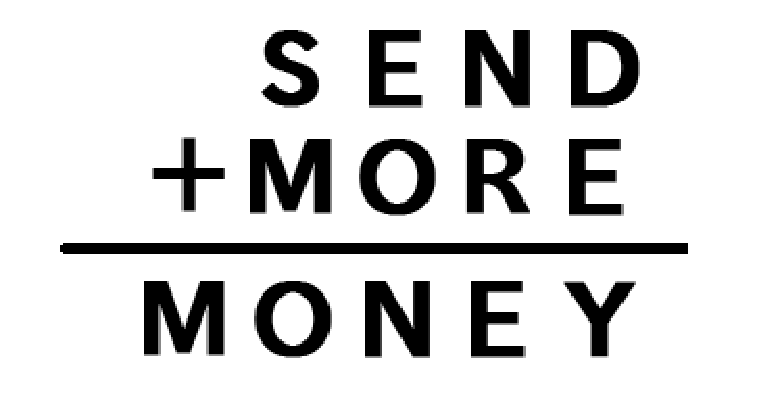
\epsfig{file=Figures/send-more-money.pdf, scale=0.4}}

\caption{A cryptarithmetic puzzle}
\label{fig:send-more-money.pdf}
\end{figure}

Your task is to reformulate this puzzle as a constraint
programming problem.  You should start from the following notebook:
\\[0.2cm]
\hspace*{0.3cm}
\href{https://github.com/karlstroetmann/Logic/blob/master/Python/Chapter-5/Crypto-Arithmetic.ipynb}{\texttt{github.com/karlstroetmann/Logic/blob/master/Python/Chapter-5/Crypto-Arithmetic.ipynb}}
\\[0.2cm]
It is importtant that you add the digits one by one as in elementary school.  This way, the addition is
separated into a number of constraints that can then be solved by backtracking.  \eox

\section{Solving Search Problems by Constraint Programming}
In this section we show how we can formulate certain \blue{search problems} as \mytt{CSP}s.
We will explain our method by solving the
\href{https://en.wikipedia.org/wiki/Missionaries_and_cannibals_problem}{missionaries and cannibals problem},
which is explained in the following:
Three missionaries and three infidels have to cross a river in order to get to a church where the infidels can
be baptized.  According to ancient catholic mythology, baptizing the infidels is necessary to save them from
the eternal tortures of hell fire. In order to cross the river, the missionaries and infidels have a small boat
available that can take at most two passengers. If at any moments at any shore there are more infidels than
missionaries, then the missionaries have a problem, since the infidels have a diet that is rather unhealthy for
the missionaries. 

In order to solve this problem via constraint programming, we first introduce the notion of a
\blue{symbolic transition system}.

\begin{Definition}[Symbolic Transition System]
  A symbolic transition system is a 6-tuple
  \\[0.2cm]
  \hspace*{1.3cm}
  $\mathcal{T} = \langle \mathcal{V}, \mathcal{U}, \mathtt{Start}, \mathtt{Goal}, \mathtt{Invariant}, \mathtt{Transition} \rangle$
  \\[0.2cm]
  such that:
  \begin{enumerate}[(a)]
  \item $\mathcal{V}$ is a set of variables.

        These variables are strings.  For every variable $x \in \mathcal{V}$ there is a \blue{primed}
        variable $x'$ which does not occur in $\mathcal{V}$.  The set of these primed variables is denoted as
        $\mathcal{V}'$.
  \item $\mathcal{U}$ is a set of values that these variables can take.
  \item \texttt{Start}, \texttt{Goal}, and \texttt{Invariant} are first-order formulas such that all free
         variables occurring in these formulas are elements from the set $\mathcal{V}$.
         \begin{itemize}
         \item \texttt{Start} describes the initial state of the transition system.
         \item \texttt{Goal} describes a state that should be reached by the transition system.
         \item \texttt{Invariant} is a formula that has to be true for every state of the transition system.
         \end{itemize}
  \item \texttt{Transition} is a first-order formula.  The free variables of this formula are elements of
        the set $\mathcal{V} \cup \mathcal{V}'$, i.e.~they are either variables from the set $\mathcal{V}$
        or they are primed variables from the set $\mathcal{V}'$.

        The formula \texttt{Transition} describes how the variables in the transition system change during a
        state transition.  The primed variables refer to the values of the original variables after the
        state transition.
  \end{enumerate}
\end{Definition}
Every \blue{state} of a transition system is a mapping of the variable to values.
The idea is that the formula \texttt{Start} describes the start state of our search problem, \texttt{Goal}
describes the state that we want to reach, while \texttt{Invariant} is a formula that must be true initially
and that has to remain true after every transition of our system.


In order to clarify this definition we show how the \emph{missionaries and cannibals} problem can be formulated as
a symbolic transition system.
\begin{enumerate}[(a)]
\item $\mathcal{V} := \{ \mathtt{M}, \mathtt{C}, \mathtt{B} \}$.

      The value of \texttt{M} is the number of missionaries on the western shore, the value of \texttt{C} is
      the number of infidels on that shore, while the value of \texttt{B} is the number of boats on the western
      shore.
\item $\mathcal{U} := \{ 0, 1, 2, 3 \}$.
\item $\texttt{Start} := (\mathtt{M} = 3 \wedge \mathtt{C} = 3 \wedge \mathtt{B} = 1)$.

      At the beginning, there are 3 missionaries, 3 infidels, and 1 boat on the western shore.
\item $\texttt{Goal}  := (\mathtt{M} = 0 \wedge \mathtt{C} = 0 \wedge B = 0)$.

      The goal is to transfer everybody to the eastern shore.  If the goal is reached, the number of
      missionaries, infidels, and boats on the western shore will be $0$.
\item $\texttt{Invariant} := \bigl((\mathtt{M} = 3 \vee \mathtt{M} = 0 \vee \mathtt{M} = \mathtt{C}) \;\wedge\; \mathtt{B} \leq 1\bigr)$.

      The first part of the invariant, i.e.~the formulas $\mathtt{M} = 3 \vee \mathtt{M} = 0 \vee \mathtt{M} = \mathtt{C}$,
      describes those states where the missionaries are not threatened by the infidels.
      \begin{itemize}
      \item $\mathtt{M} = 3$: All missionaries are on the western shore.
      \item $\mathtt{M} = 0$: All missionaries are together on the eastern shore.
      \item $\mathtt{M} = \mathtt{C}$: On both shores the numbers of missionaries and cannibals are the same.

            If neither $\mathtt{M} = 3$ nor $\mathtt{M} = 0$ holds, then the number of missionaries and
            cannibals have to be the same on the western shore, because if, for example, there were more
            missionaries on the western shore than cannibals, then there would be less missionaries than
            cannibals on the eastern shore and hence there would be a problem.
      \end{itemize}
      The condition $\mathtt{B} \leq 1$ is needed because there is just one boat, but the set $\mathcal{U}$ of
      values also includes the numbers $2$ and $3$.
\item $\texttt{Transition} :=
      \begin{array}[t]{cl}
         &  \mathtt{B}' = 1 - \mathtt{B}   \\[0.2cm]
        \wedge & \bigl(\mathtt{B} = 1 \;\rightarrow\; 1 \leq \mathtt{M} - \mathtt{M}'  + \mathtt{C} - \mathtt{C}' \leq 2 \;\wedge\;
        \mathtt{M}' \leq \mathtt{M} \;\wedge\; \mathtt{C}' \leq \mathtt{C}\bigr) \\[0.2cm]
        \wedge & \bigl(\mathtt{B} = 0 \;\rightarrow\; 1 \leq \mathtt{M}' - \mathtt{M}  + \mathtt{C}' - \mathtt{C} \leq 2 \;\wedge\;
                \mathtt{M}' \geq \mathtt{M} \;\wedge\; \mathtt{C}' \geq \mathtt{C}\bigr) 
      \end{array}
      $

      Let us explain the details of this formula:
      \begin{itemize}
      \item $\mathtt{B}' = 1 - \mathtt{B}$

            If the boat is initially on the western shore, i.e. $\texttt{B} = 1$, it will be on the eastern
            shore afterwards, i.e. we will then have $\texttt{B}' = 0$.  If, instead, the boat is initially on
            the eastern shore, i.e. $\texttt{B} = 0$, it will be on the western
            shore afterwards and then we have $\texttt{B}' = 1$.
      \item $\mathtt{B} = 1 \;\rightarrow\; 1 \leq \mathtt{M} - \mathtt{M}'  + \mathtt{C} - \mathtt{C}' \leq 2 \;\wedge\;
             \mathtt{M}' \leq \mathtt{M} \;\wedge\; \mathtt{C}' \leq \mathtt{C}$


            If the boat is initially on the western shore, then afterwards the number of missionaries and
            infidels will decrease, as they leave for the eastern shore.  In this case $\texttt{M} - \texttt{M}'$
            is the number of missionaries on the boat, while $\texttt{C} - \texttt{C}'$ is the number of
            infidels.  The sum of these numbers has to be between $1$ and $2$ because the boat can not travel
            empty and can take at most two passengers.

            The condition $\mathtt{M}' \leq \mathtt{M}$ is true because when missionaries are traveling from
            the western shore to the eastern shore, the number of missionaries on the western shore can not
            increase.  Similarly,  $\mathtt{C}' \leq \mathtt{C}$ has to be true.
      \item $\mathtt{B} = 0 \;\rightarrow\; 1 \leq \mathtt{M}' - \mathtt{M}  + \mathtt{C}' - \mathtt{C} \leq 2 \;\wedge\;
            \mathtt{M}' \geq \mathtt{M} \;\wedge\; \mathtt{C}' \geq \mathtt{C}$

            This formula describes the transition from the eastern shore to the western shore and is analogous
            to the previous formula.
      \end{itemize}
\end{enumerate}


\begin{figure}[!ht]
\centering
\begin{Verbatim}[frame         = single, 
                 framesep      = 0.3cm,
                 framerule=0.5mm,
                 rulecolor=\color{black},
                 firstnumber   = 1,
                 numbers       = left,
                 numbersep     = 0.3cm,
                 xleftmargin   = 0.8cm,
                 xrightmargin  = 0.8cm,
                 commandchars  = \\\{\},
                 codes         = {\catcode`$=3\catcode`^=7}
               ] 
\colorbox{sepia}{def start(M, C, B):                                                       }
\colorbox{sepia}{    return M == 3 and C == 3 and B == 1                                   }
\colorbox{sepia}{                                                                          }
\colorbox{sepia}{def goal(M, C, B):                                                        }
\colorbox{sepia}{    return M == 0 and C == 0 and B == 0                                   }
\colorbox{sepia}{                                                                          }
\colorbox{sepia}{def invariant(M, C, B):                                                   }
\colorbox{sepia}{    return (M == 0 or M == 3 or M == C) and B <= 1                        }
\colorbox{sepia}{                                                                          }
\colorbox{sepia}{def transition(M$\alpha$, C$\alpha$, B$\alpha$, M$\beta$, C$\beta$, B$\beta$):                                   }
\colorbox{sepia}{    if not (B$\beta$ == 1 - B$\alpha$):                                                }
\colorbox{sepia}{        return False                                                      }
\colorbox{sepia}{    if B$\alpha$ == 1:                                                           }
\colorbox{sepia}{        return 1 <= M$\alpha$ - M$\beta$ + C$\alpha$ - C$\beta$ <= 2 and M$\beta$ <= M$\alpha$ and C$\beta$ <= C$\alpha$     }
\colorbox{sepia}{    else:                                                                 }
\colorbox{sepia}{        return 1 <= M$\beta$ - M$\alpha$ + C$\beta$ - C$\alpha$ <= 2 and M$\beta$ >= M$\alpha$ and C$\beta$ >= C$\alpha$     }
\end{Verbatim}
\vspace*{-0.3cm}
\caption{Coding the \emph{missionaries and cannibals problem} as a symbolic transition system.}
\label{fig:Missionaries-STS.ipynb}
\end{figure}

%$
Figure \ref{fig:Missionaries-STS.ipynb} shows how the \emph{missionaries and cannibals problem} can be
represented as a symbolic transition system in \textsl{Python}.  In the function \texttt{transition} 
we use the following convention: Since variables cannot be primed in
\textsl{Python} we append the character $\alpha$ to the names of the original
variables from the set $\mathcal{V}$, while we append $\beta$ to these names to get the primed versions of the
corresponding variable.


\begin{figure}[!ht]
\centering
\begin{minted}[ frame         = lines, 
                framesep      = 0.3cm, 
                firstnumber   = 1,
                bgcolor       = sepia,
                numbers       = left,
                numbersep     = -0.2cm,
                xleftmargin   = 0.0cm,
                xrightmargin  = 0.0cm,
              ]{python3}
    def flatten(LoL):
        return [x for L in LoL for x in L]
                    
    def missionaries_CSP(n):
        "Returns a CSP encoding the problem."
        Lists        = [[f'M{i}', f'C{i}', f'B{i}'] for i in range(n+1)]
        Variables    = flatten(Lists)
        Values       = { 0, 1, 2, 3 }
        Constraints  = {  'start(M0, C0, B0)'      }  # start state
        Constraints |= { f'goal(M{n}, C{n}, B{n})' }  # goal state
        for i in range(n):
            Constraints.add(f'invariant(M{i}, C{i}, B{i})')
            Constraints.add(f'transition(M{i}, C{i}, B{i}, M{i+1}, C{i+1}, B{i+1})')
        return Variables, Values, Constraints
        
    def find_solution():
        n = 1
        while True:
            print(n)
            CSP = missionaries_CSP(n)
            Solution = solve(CSP)
            if Solution != None:
                return n, Solution
            n += 2
\end{minted}
\vspace*{-0.3cm}
\caption{Turning the symbolic transition system into a \textsc{Csp}.}
\label{fig:Missionaries-STS.ipynb-2}
\end{figure}

Figure \ref{fig:Missionaries-STS.ipynb-2} shows how we can turn the symbolic transition system into a
\textsc{Csp}.
\begin{enumerate}
\item The function $\texttt{flatten}(\texttt{LoL})$ receives a list of lists $\texttt{LoL}$ as its argument.
       This list has the form
       \\[0.2cm]
       \hspace*{1.3cm}
       $\texttt{LoL} = [L_1, \cdots, L_k]$
       \\[0.2cm]
       where the $L_i$ are lists for $i=1,\cdots,k$.
       
       It returns the list
       \\[0.2cm]
       \hspace*{1.3cm}
       $L_1 + \cdots + L_k$,
       \\[0.2cm]
       i.e.~it concatenates the lists that are elements of \texttt{Lol} and returns the resulting list.
\item The function $\mathtt{missionaries\_CSP}(n)$ receives a natural number $n$ as its argument.
       It returns a \textsc{Csp} that has a solution iff there is a solution of the \emph{missionaries and cannibals}
       problem that crosses the river exactly $n$ times.  It uses the variables
       \\[0.2cm]
       \hspace*{1.3cm}
       $\mathtt{M}_i$, $\mathtt{C}_i$, and $\mathtt{B}_i$, where $i=0,\cdots,n$.
       \\[0.2cm]
       $\mathtt{M}_i$ is the number of missionaries on the western shore after the boat has crossed the river
       $i$ times. The variables $\mathtt{C}_i$ and $\texttt{B}_i$ denote the number of infidels and boats
       respectively.

       Line 12 ensures that the invariant of the transition system is valid after every crossing of the boat.
       Line 13 describes the mechanics of the crossing.
\item The function \texttt{find\_solution} tries to find a natural number $n$ such that problem can be solved
       with $n$ crossings. As the number of crossings has to be odd, we increment $n$ by
       two at the end of the \texttt{while} loop.

       The function \texttt{find\_solution} needs less than 2 seconds to find the solution.
\end{enumerate}

\exerciseEng
An agricultural economist has to sell a \blue{wolf}, a \blue{goat}, and a \blue{cabbage}
on a market place.  In order to reach the market place, she has to cross a river.  The
boat that she can use is so small that it can only accommodate either the goat, the wolf,
or the cabbage in addition to the agricultural economist herself.  Now if the agricultural
economist leaves the wolf alone with the goat, the wolf will eat the goat.  If, instead,
the agricultural economist leaves the goat with the cabbage, the goat will eat the
cabbage.  Is it possible for the agricultural economist to develop a schedule that allows
her to cross the river without either the goat or the cabbage being eaten?

Encode this problem as a \blue{symbolic transition system} and then solve it with the help
of the constraints solver developed earlier.  Assume that the
problem can be solved with $n\in\mathbb{N}$ crossing of the river.  Use the following
variables:
\begin{itemize}
\item $\texttt{F}i$ for $i\in\{0,\cdots,n\}$ is the number of farmers on the western shore after the 
      $i^{\textrm{th}}$ crossing.
\item $\texttt{W}i$ for $i\in\{0,\cdots,n\}$ is the number of wolves on the western shore after the 
      $i^{\textrm{th}}$ crossing.
\item $\texttt{G}i$ for $i\in\{0,\cdots,n\}$ is the number of goats on the western shore after the 
      $i^{\textrm{th}}$ crossing.
\item $\texttt{C}i$ for $i\in\{0,\cdots,n\}$ is the number of cabbages on the western shore after the 
      $i^{\textrm{th}}$ crossing.
\end{itemize}
You should start from the following notebook:
\\[0.2cm]
\hspace*{-0.5cm}
\href{https://github.com/karlstroetmann/Logic/blob/master/Python/Chapter-5/Wolf-Goat-Cabbage-STS.ipynb}{\texttt{github.com/karlstroetmann/Logic/blob/master/Python/Chapter-5/Wolf-Goat-Cabbage-STS.ipynb}}
\eox

\section{The Z3 Solver}
We proceed with a discussion of the solver
\href{https://www.microsoft.com/en-us/research/project/z3-3/}{Z3}, which has beed developd
at Microsoft.  Z3 implements most of the state-of-the-art constraint solving algorithms
and is exceptionally powerful.  We introduce Z3 via a series of examples.

\subsection{A Simple Text Problem}
The following is a simple text problem from my old $8^{\textrm{th}}$ grade math book.
\textsl{
  \begin{itemize}
  \item I have as many brothers as I have sisters.
  \item My sister has twice as many brothers as she has sisters.
  \item How many children does my father have?
  \end{itemize}}
\noindent
In order to solve this puzzle we need two additional assumptions.
\begin{enumerate}
\item My father has no illegitimate children.
\item All of my fathers children identify themselves as either male or female.
\end{enumerate}
Strangely, in my old math book these assumptions have not been mentioned.

We can now infer the number of children.
If we denote the number of \blue{boys} by the variable $b$ and the number of \blue{girls}
by the variable $g$, the problem statements are equivalent to the following two equations:
\\[0.2cm]
\hspace*{1.3cm}
$b - 1 = g$ \quad and \quad $2 \cdot (g - 1) = b$.
\\[0.2cm]
Before we can start to solve this problem, we have to install \texttt{Z3} via \texttt{pip} using the following
command:  
\\[0.2cm]
\hspace*{1.3cm}
\texttt{pip install z3-solver}


\begin{figure}[!ht]
\centering
\begin{minted}[ frame         = lines, 
                 framesep      = 0.3cm, 
                 firstnumber   = 1,
                 bgcolor       = sepia,
                 numbers       = left,
                 numbersep     = -0.2cm,
                 xleftmargin   = 0.8cm,
                 xrightmargin  = 0.8cm,
               ]{python3}             
    import z3
    
    boys  = z3.Int('boys')
    girls = z3.Int('girls')
    
    S = z3.Solver()
    
    S.add(boys - 1 == girls)
    S.add(2 * (girls - 1) == boys)
    S.check()
    Solution = S.model()
    
    b = Solution[boys ].as_long()
    g = Solution[girls].as_long()
    
    print(f'My father has {b + g} children.')
\end{minted}
\vspace*{-0.3cm}
\caption{Solving a simple text problem.}
\label{fig:Brothers-and-Sisters.ipynb}
\end{figure}

\noindent
Figure \ref{fig:Brothers-and-Sisters.ipynb} on page \pageref{fig:Brothers-and-Sisters.ipynb} shows how we can
solve the given problem using the \textsl{Python}
interface of Z3.
\begin{enumerate}
\item In line 1 we import the module \texttt{z3} so that we can use the Python \textsc{Api} of Z3.
      The documentation of this \textsc{Api} is available at the following address:
      \\[0.2cm]
      \hspace*{1.3cm}
      \href{https://ericpony.github.io/z3py-tutorial/guide-examples.htm}{https://ericpony.github.io/z3py-tutorial/guide-examples.htm}
      \\[0.2cm]
      However, there is no need for you to consult this documentation as we will only use a very small part of
      the \textsc{Api} of \texttt{Z3} in this lecture. 
\item Lines 3 and 4 creates the \texttt{Z3} variables \mytt{boys} and \mytt{girls} as integer valued variables.
      The function \mytt{Int} takes one argument, which has to be a string.  This string is the name of the
      variable.  We store these variables in Python variables of the same name.  It would be possible to use
      different names for the Python variables, but that would be very confusing.
\item Line 6 creates an object of the class \texttt{Solver}.  This is the constraint solver provided by
      \texttt{Z3}.
    \item Lines 8 and 9 add the constraints expressing that
      \begin{enumerate}[(a)]
      \item the number of girls is one less than the number of boys \quad and 
      \item that my sister has twice as many brothers as she has sisters 
      \end{enumerate}
      as constraints to the solver \texttt{S}.
\item In line 10 the method \mytt{check} examines whether the given set of constraints is satisfiable.
      In general, this method returns one of the following results:
      \begin{enumerate}[(a)]
      \item \mytt{sat} is returned if the problem is solvable, (\mytt{sat} is short for \emph{satisfiable})
      \item \mytt{unsat} is returned if the problem is unsolvable,
      \item \mytt{unknown} is returned if \texttt{Z3} is not powerful enough to solve the given problem.
      \end{enumerate}
\item Since in our case the method \mytt{check} returns \texttt{sat}, we can extract the solution that is
      computed via the method \mytt{model} in line 11.  
\item In order to extract the values that have been computed by \texttt{Z3} for the variables \mytt{boys} and
      \mytt{girls}, we can use dictionary syntax and write \mytt{Solution[boys]} and
      \mytt{Solution[girls]} to extract these values.  However, these values are not stored as integers but
      rather as objects of the class \mytt{IntNumRef}, which is some internal class of \texttt{Z3} to store
      integers.  This class provides the method \mytt{as\_long} that converts its argument into an integer number.
\end{enumerate}

\exerciseEng
Solve the following text problem using \texttt{Z3}.
\textsl{
  \begin{enumerate}[(a)]
  \item A Japanese deli offers both
        \href{https://www.discovermagazine.com/health/hearty-penguin-steaks-the-old-school-explorers-salve-for-scurvy}{penguins}
        and \href{http://fancytoast.blogspot.com/2007/04/parrot-three-ways.html}{parrots}.  
  \item A parrot and a penguin together cost 666 bucks.
  \item The penguin costs 600 bucks more than the parrot.  
  \end{enumerate}}
  \noindent
  \textbf{What is the price of the parrot?} You may assume that the prizes of these
  delicacies are integer valued.
  You should start from the following notebook:
\\[0.2cm]
\hspace*{0.0cm}
\href{https://github.com/karlstroetmann/Logic/blob/master/Python/Chapter-5/Parrot-and-Penguin.ipynb}{\texttt{github.com/karlstroetmann/Logic/blob/master/Python/Chapter-5/Parrot-and-Penguin.ipynb}}
\eox

\exerciseEng
Solve the following text problem using \texttt{Z3}.
\textsl{
  \begin{enumerate}[(a)]
  \item  A train travels at a uniform speed for 360 miles.  
  \item  The train would have taken 48 minutes less to travel the same distance 
         if it had been faster by 5 miles per hour.
  \end{enumerate}}
\noindent
\textbf{Find the speed of the train!}

\noindent
\textbf{Hints:}
\begin{enumerate}[(a)]
\item As the speed is a real number you should declare this variable via the \texttt{Z3} function \texttt{Real} instead of using
      the function \texttt{Int}.
\item Be careful to not mix up different units. In particular, the time 48 minutes should be expressed as a
      fraction of an hour.
\item When you formulate the information given above, you will get a system of \textbf{non-linear} equations,
      which is equivalent to a quadratic equation.  This quadratic equation has two different solutions.
      One of these solutions is negative.  In order to exclude the negative solution you need to add a
      constraint stating that the speed of the train has to be greater than zero.
\end{enumerate}
You should start from the following notebook:
\\[0.2cm]
\hspace*{0.8cm}
\href{https://github.com/karlstroetmann/Logic/blob/master/Python/Chapter-5/Train-Z3.ipynb}{\texttt{github.com/karlstroetmann/Logic/blob/master/Python/Chapter-5/Train-Z3.ipynb}}
\eox

\subsection{The Knight's Tour}
In this subsection we will solve the puzzle \href{https://en.wikipedia.org/wiki/Knight%27s_tour}{The Knight's Tour} 
using \texttt{Z3}.  This puzzle asks whether it is possible for a knight to visit all 64 squares of a chess board
in 63 moves.  We will start the tour in the upper left corner of the board.  

In order to model this puzzle as a constraint satisfaction problem we first have to decide on the variables
that we want to use. The idea is to have 64 variables that describe the position of the knight after its
$i^{\mathrm{th}}$ move where $i=0,1,\cdots,63$.  However, it turns out that it is best to split the values of these positions up into a
row and a column.  If we do this, we end up with 128 variables of the form
\\[0.2cm]
\hspace*{1.3cm}
$\mathtt{R}_i$ and $\mathtt{C}_i$ \quad for $i \in \{0, 1, \cdots, 63\}$.
\\[0.2cm]
Here $\mathtt{R}_i$ denotes the row of the knight after its $i^{\mathrm{th}}$ move, while $\mathtt{C}_i$
denotes the corresponding column.  
Next, we have to formulate the constraints.  In this case, there are two kinds of constraints:
\begin{enumerate}
\item We have to specify that the move from the position $\langle \mathtt{R}_i, \mathtt{C}_i \rangle$
      to the position $\langle \mathtt{R}_{i+1}, \mathtt{C}_{i+1} \rangle$ is legal move for a knight.
      In chess, there are two ways for a knight to move:
      \begin{enumerate}[(a)]
      \item The knight can move two squares horizontally left or right followed by moving vertically
            one square up or down, or
      \item the knight can move two squares vertically up or down followed by moving
            one square left or right.
      \end{enumerate}
      Figure \ref{fig:knight-moves.png} shows all legal moves of a knight that is positioned in the square \texttt{e4}.
      Therefore, a formula that expresses that the $i^{\mathrm{th}}$ move is a legal move of the knight is a disjunction
      of the following eight formulas that each describe one possible way for the knight to move:
      \begin{enumerate}
      \item $\mathtt{R}_{i+1} = \mathtt{R}_{i} + 2 \;\wedge\; \mathtt{C}_{i+1} = \mathtt{C}_{i} + 1$,
      \item $\mathtt{R}_{i+1} = \mathtt{R}_{i} + 2 \;\wedge\; \mathtt{C}_{i+1} = \mathtt{C}_{i} - 1$, 
      \item $\mathtt{R}_{i+1} = \mathtt{R}_{i} - 2 \;\wedge\; \mathtt{C}_{i+1} = \mathtt{C}_{i} + 1$, 
      \item $\mathtt{R}_{i+1} = \mathtt{R}_{i} - 2 \;\wedge\; \mathtt{C}_{i+1} = \mathtt{C}_{i} - 1$, 
      \item $\mathtt{R}_{i+1} = \mathtt{R}_{i} + 1 \;\wedge\; \mathtt{C}_{i+1} = \mathtt{C}_{i} + 2$, 
      \item $\mathtt{R}_{i+1} = \mathtt{R}_{i} + 1 \;\wedge\; \mathtt{C}_{i+1} = \mathtt{C}_{i} - 2$, 
      \item $\mathtt{R}_{i+1} = \mathtt{R}_{i} - 1 \;\wedge\; \mathtt{C}_{i+1} = \mathtt{C}_{i} + 2$, 
      \item $\mathtt{R}_{i+1} = \mathtt{R}_{i} - 1 \;\wedge\; \mathtt{C}_{i+1} = \mathtt{C}_{i} - 2$. 
      \end{enumerate}
\item Furthermore, we have to specify that the position  $\langle \mathtt{R}_i, \mathtt{C}_i \rangle$ is
      different from the position  $\langle \mathtt{R}_j, \mathtt{C}_j \rangle$ if $i \not= j$.
\end{enumerate}


\begin{figure}[!ht]
  \centering
  \framebox{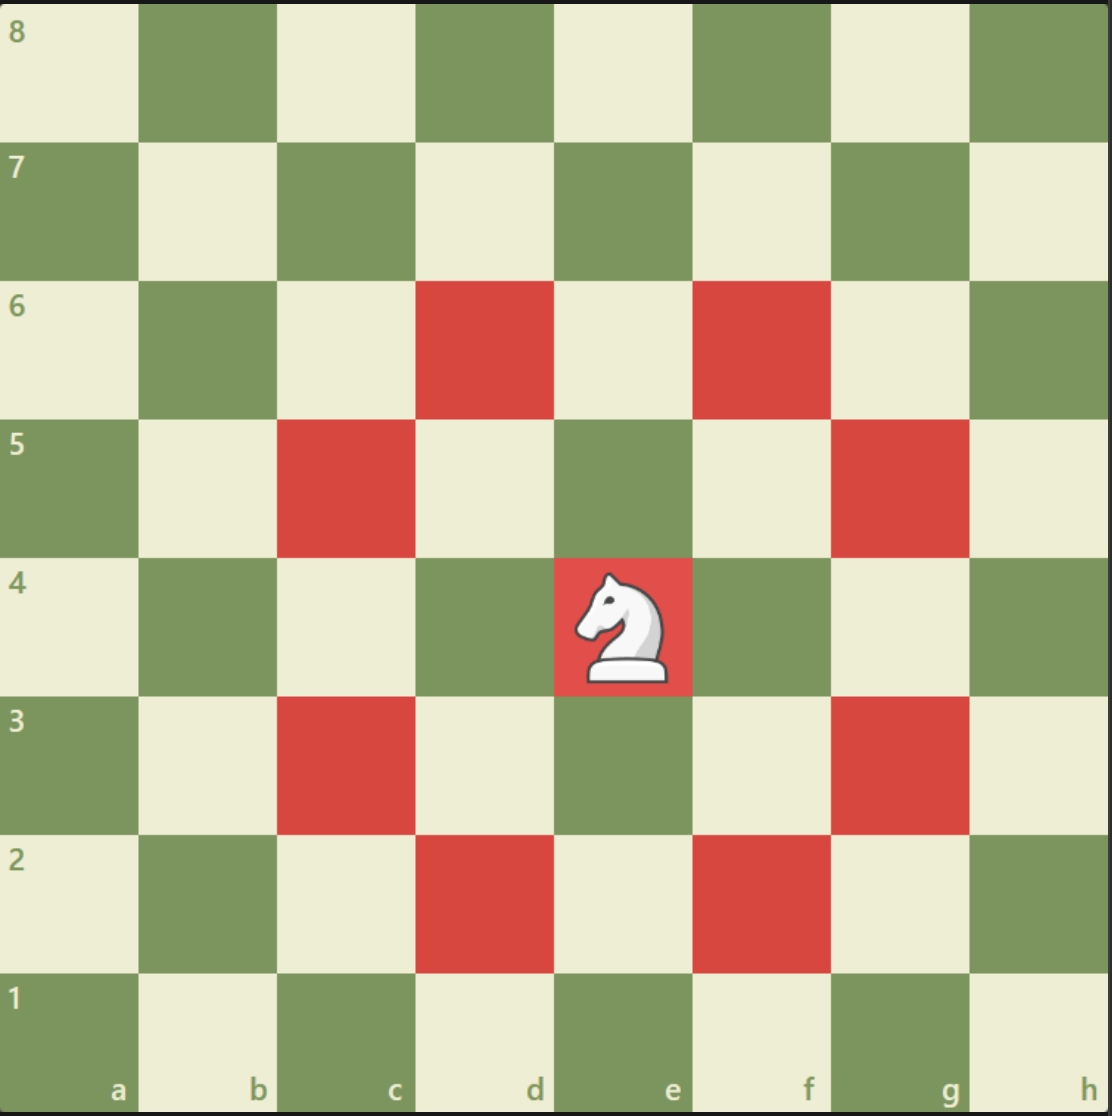
\epsfig{file=Figures/knight-moves.png, scale=0.5}} 
  \caption{The moves of a knight, courtesy of \href{https://www.chess.com/}{chess.com}.}
  \label{fig:knight-moves.png}
\end{figure}

\begin{figure}[!ht]
\centering
\begin{minted}[ frame         = lines, 
                 framesep      = 0.3cm, 
                 firstnumber   = 1,
                 bgcolor       = sepia,
                 numbers       = left,
                 numbersep     = -0.2cm,
                 xleftmargin   = 0.0cm,
                 xrightmargin  = 0.0cm,
               ]{python3}
    import z3
               
    def row(i): return f'R{i}'
    def col(i): return f'C{i}'
    
    def is_knight_move(row, col, rowX, colX):
        Formulas = set()
        S = {1, 2, -1, -2}
        DeltaSet = {(x, y) for x in S for y in S if abs(x) != abs(y)}
        for delta_r, delta_c in DeltaSet:
            Formulas.add(z3.And(rowX == row + delta_r, colX == col + delta_c))
        return z3.Or(Formulas)
            
    def all_different(Rows, Cols):
        Result = set()
        for i in range(62+1):
            for j in range (i+1, 63+1):
                Result.add(z3.Or(Rows[i] != Rows[j], Cols[i] != Cols[j]))
        return Result
            
    def all_constraints(Rows, Cols):
        Constraints = all_different(Rows, Cols)
        Constraints.add(Rows[0] == 0)
        Constraints.add(Cols[0] == 0)
        for i in range(62+1):
            Constraints.add(is_knight_move(Rows[i], Cols[i], Rows[i+1], Cols[i+1]))
        for i in range(63+1):
            Constraints.add(Rows[i] >= 0) 
            Constraints.add(Cols[i] >= 0) 
        return Constraints
\end{minted}
\vspace*{-0.3cm}
\caption{The Knight's Tour: Computing the constraints.}
\label{fig:Knight's Tour with Z3.ipynb-1}
\end{figure}



Figure \ref{fig:Knight's Tour with Z3.ipynb-1} shows how we can formulate the puzzle using \texttt{Z3}.
\begin{enumerate}
\item In line 1 we import the library \texttt{z3}.
 
\item We define the auxiliary functions \texttt{row} and \texttt{col} in line 3 and 4.
      Given a natural number $i$, the expression $\mathtt{row}(i)$ returns the string $\texttt{'R}i\texttt{'}$
      and  $\mathtt{col}(i)$ returns the string  $\texttt{'C}i\texttt{'}$.  These strings in turn represent the
      variables $\mathtt{R}_i$ and $\mathtt{C}_i$.
\item The function \texttt{is\_knight\_move} takes four parameters:
      \begin{enumerate}
      \item \texttt{row} is a \texttt{Z3} variable that specifies the row of the position of the knight before
            the move. 
      \item \texttt{col} is a \texttt{Z3} variable that specifies the column of the position of the knight
            before the move. 
      \item \texttt{rowX} is a \texttt{Z3} variable that specifies the row of the position of the knight after
            the move. 
      \item \texttt{colX} is a \texttt{Z3} variable that specifies the column of the position of the knight
            after the move. 
      \end{enumerate}
      The function checks whether the move from position 
      $\langle \mathtt{R}_i, \mathtt{C}_i \rangle$ to the position $\langle \mathtt{R}_{i+1}, \mathtt{C}_{i+1} \rangle$
      is a legal move for a knight.  In line 13 we use the fact that the function \texttt{z3.Or}
      can take any number of arguments.  If \texttt{Formulas} is the set 
      \\[0.2cm]
      \hspace*{1.3cm}
      $\texttt{Formulas} = \{f_1, \cdots, f_n\}$,
      \\[0.2cm]
      then the notation \texttt{z3.Or(*Formulas)} is expanded into the call
      \\[0.2cm]
      \hspace*{1.3cm}
      $\texttt{z3.Or}(f_1, \cdots, f_n)$,
      \\[0.2cm]
      which computes the logical disjunction
      \\[0.2cm]
      \hspace*{1.3cm}
      $f_1 \vee \cdots \vee f_n$.
\item The function \texttt{all\_different} takes two parameters:
      \begin{enumerate}[(a)]
      \item \texttt{Rows} is a list of \texttt{Z3} variables. The \texttt{Z3} variable \texttt{Rows[i]}
            specifies the row of the position of the knight after the $i^{\textrm{th}}$ move. 
      \item \texttt{Cols} is a list of \texttt{Z3} variables. The \texttt{Z3} variable \texttt{Cols[i]}
            specifies the column of the position of the knight after the $i^{\textrm{th}}$ move. 
      \end{enumerate}
      The function computes a set of formulas that state that the positions
      $\langle \mathtt{R}_i, \mathtt{C}_i \rangle$ for $i=0,1\cdots, 63$ are all different from each other.
      Note that the position $\langle \mathtt{R}_i, \mathtt{C}_i \rangle$ is different from the position
      $\langle \mathtt{R}_j, \mathtt{C}_j \rangle$ iff $R_i$ is different from $R_j$ or $C_i$ is different from
      $C_j$. 
\item The function \texttt{all\_constraints} computes the set of all constraints.
      The parameters for this function are the same as those for the function \texttt{all\_different}.
      In addition to the constraints already discussed this function specifies that the knight starts
      its tour at the upper left corner of the board.

      Furthermore, there are constraints that the variables $\mathtt{R}_i$ and $\mathtt{C}_i$ are all
      non-negative.  These constraints are needed as we will model the variables with bit vectors of length 4.
      These bit vectors store integers in
      \href{https://en.wikipedia.org/wiki/Two%27s_complement}{two's complement} representation.
      In two's complement representation of a bit vector of length 4 we can model integers from the set
      $\{-8, \cdots, 7\}$.  If we add the number $1$ to a 4-bit bit vector $v$ that represents the number $7$,
      then an overflow will occur and the result will be $-8$ instead of $8$. This could happen in the
      additions that are performed in the formulas computed by the function \texttt{is\_knight\_move}.
      We can exclude these cases by adding the constraints that all variables are non-negative.
\end{enumerate}

\begin{figure}[!ht]
\centering
\begin{minted}[ frame         = lines, 
                 framesep      = 0.3cm, 
                 firstnumber   = 1,
                 bgcolor       = sepia,
                 numbers       = left,
                 numbersep     = -0.2cm,
                 xleftmargin   = 0.8cm,
                 xrightmargin  = 0.8cm,
               ]{python3}
    def solve():
        Rows = [z3.BitVec(row(i), 4) for i in range(63+1)]
        Cols = [z3.BitVec(col(i), 4) for i in range(63+1)]
        Constraints = all_constraints(Rows, Cols)
        S = z3.Solver()
        S.add(Constraints)
        result = str(S.check())
        if result == 'sat':
            Model    = S.model()
            Solution = (  { row(i): Model[Rows[i]] for i in range(63+1) } 
                        | { col(i): Model[Cols[i]] for i in range(63+1) })
            return Solution
        elif result == 'unsat':
            print('The problem is not solvable.')
        else:
            print('Z3 cannot determine whether the problem is solvable.')
\end{minted}
\vspace*{-0.3cm}
\caption{The function \texttt{solve}.}
\label{fig:Knight's Tour with Z3.ipynb-2}
\end{figure}

\begin{figure}[!ht]
  \centering
  \framebox{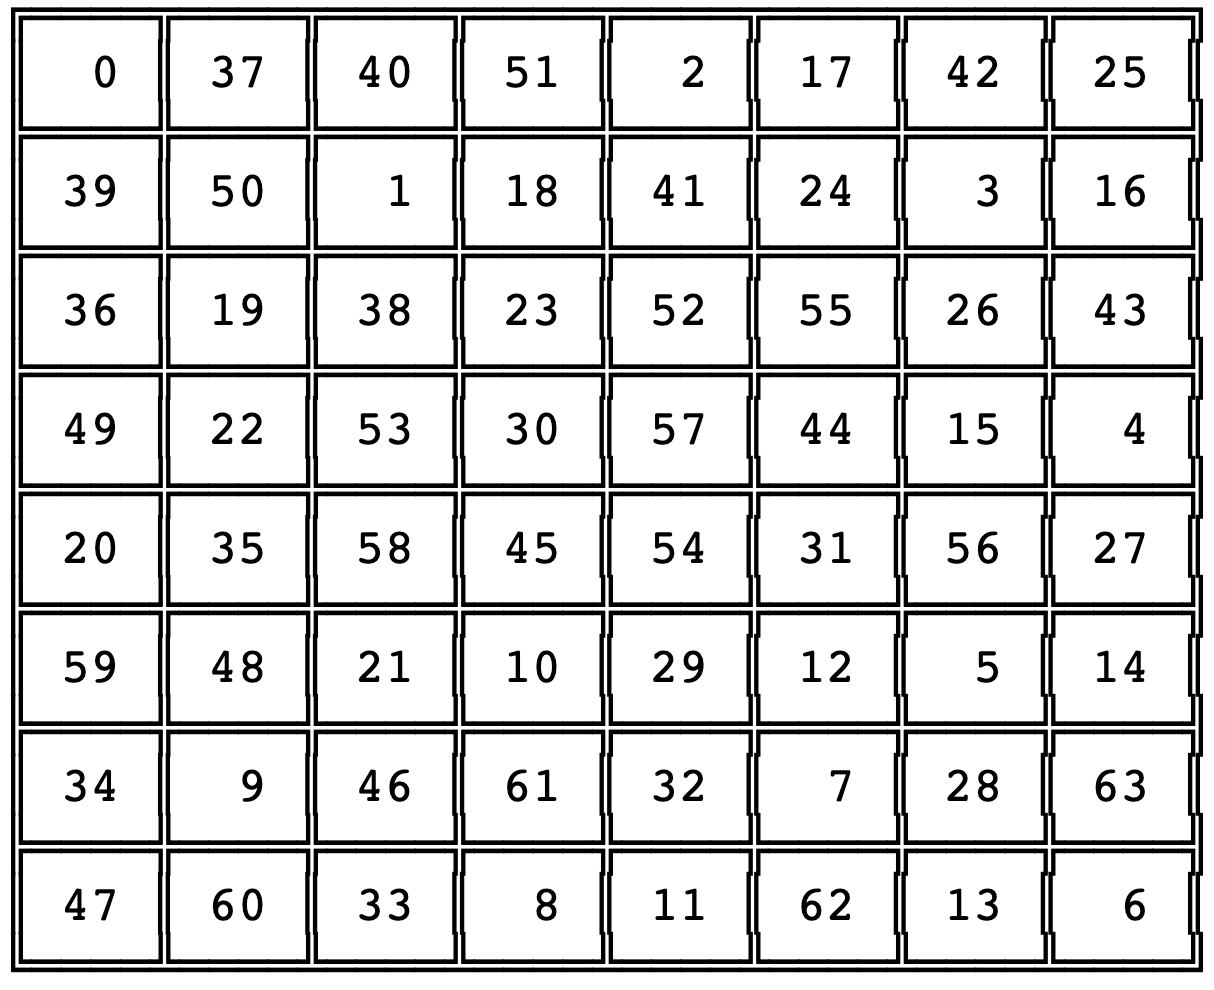
\epsfig{file=Figures/knights-problem.png, scale=0.5}} 
  \caption{A solution of the knight's problem.}
  \label{fig:knights-problem.png}
\end{figure}

Finally, the function \texttt{solve} that is shown in Figure \ref{fig:Knight's Tour with Z3.ipynb-2} on page
\pageref{fig:Knight's Tour with Z3.ipynb-2} can be used to solve the puzzle.
The purpose of the function \texttt{solve} is to construct a \textsc{Csp} encoding the puzzle and to find a
solution of this \textsc{Csp} unsing \texttt{Z3}.
If successful, it returns a dictionary that maps every variable name to the corresponding value of the solution
that has been found.
\begin{enumerate}
\item In line 2 and 3 we create the \texttt{Z3} variables that specify the positions of the knight after its
      $i^{\mathrm{th}}$ move.  $\texttt{Rows}[i]$ specifies the row of the knight after the its
      $i^{\mathrm{th}}$ move, while $\texttt{Cols}[i]$ specifies the column.
\item We compute the set of all constraints in line 4.   
\item We create a solver object in line 5 and add the constraints to this solver in the following line.
\item The function \texttt{check} tries to build a model satisfying the constraints, while the function
      \texttt{model} extracts this model if it exists.
\item Finally, in line 10 and 11 we create a dictionary that maps all of our variables to the corresponding
      values that are found in the model.  Note that $\texttt{row}(i)$ returns the name of the
      \texttt{Z3} variable $\texttt{Rows}[i]$ and similarly $\mathtt{col}(i)$ returns the name of the
      \texttt{Z3} variable $\texttt{Cols}[i]$.
      This dictionary is then returned.
\end{enumerate}
Figure \ref{fig:knights-problem.png} on page \pageref{fig:knights-problem.png} shows a solution that has been
computed by the program discussed above.






\begin{table}[h]
  \centering
  \begin{tabular}{||c|c|c||c|c|c||c|c|c||}
    \hline
    \hline
      & 3 & 9 &   &   &   &   &   & 7 \\
    \hline
      &   &   & 7 &   &   & 4 & 9 & 2 \\
    \hline
      &   &   &   & 6 & 5 &   & 8 & 3 \\
    \hline
    \hline
      &   &   & 6 &   & 3 & 2 & 7 &   \\
    \hline
      &   &   &   & 4 &   & 8 &   &   \\
    \hline
    5 & 6 &   &   &   &   &   &   &   \\
    \hline
    \hline
      &   & 5 & 2 &   & 9 &   &   & 1 \\
    \hline
      & 2 & 1 &   &   &   &   & 4 &   \\
    \hline
    7 &   &   &   &   &   & 5 &   &   \\
    \hline
    \hline
  \end{tabular}
  \caption{A super hard sudoku from the magazine ``Zeit Online''.}
  \label{tab:sudoku}
\end{table}


\exerciseEng
\index{sudoku}
Table \ref{tab:sudoku} on page \pageref{tab:sudoku} shows a \href{https://en.wikipedia.org/wiki/Sudoku}{sudoku}
that I have taken from the
\href{http://sudoku.zeit.de/cgi-bin/sudoku/sudoku_kd_app_2016.pl?action=level&kd_nr=24091123601092&year=2018&month=03&day=23&level=-c+5}{Zeit Online}
magazine.
Solve this sudoku using \texttt{Z3}.  You should start with the following file:
\\[0.2cm]
\hspace*{0.0cm}
\href{https://github.com/karlstroetmann/Logic/blob/master/Python/Chapter-5/Sudoku-Z3.ipynb}{https://github.com/karlstroetmann/Logic/blob/master/Python/Chapter-5/Sudoku-Z3.ipynb}.
    \eox

\subsection{Solving Search Problems with \texttt{Z3}}
In this subsection we show how to solve a search problem using \texttt{Z3}.  The idea is to formulate the
search problem as a symbolic transition system, convert the symbolic transition system into a \textsc{Csp}, and
then solve the \textsc{Csp} using \texttt{Z3}.
We will explain our method by solving the
\href{https://en.wikipedia.org/wiki/Missionaries_and_cannibals_problem}{missionaries and cannibals problem}
that has already been discussed earlier.  

\begin{figure}[!ht]
\centering
\begin{minted}[ frame         = lines, 
                 framesep      = 0.3cm, 
                 firstnumber   = 1,
                 bgcolor       = sepia,
                 numbers       = left,
                 numbersep     = -0.2cm,
                 xleftmargin   = 0.8cm,
                 xrightmargin  = 0.8cm,
               ]{python3}
    M = z3.Int('M')
    C = z3.Int('C')
    B = z3.Int('B')
    
    def start(M, C, B):
        return z3.And(M == 3, C == 3, B == 1)
    
    def goal(M, C, B):
        return z3.And(M == 0, C == 0, B == 0)
    
    def invariant(M, C, B):
        return z3.And(z3.Or(M == 0, M == 3, M == C),
                      0 <= M, M <= 3,
                      0 <= C, C <= 3,
                      0 <= B, B <= 1)
    def transition(M, C, B, Mx, Cx, Bx):
        Formulas  = { Bx == 1 - B }
        Formulas |= { z3.Implies(B == 1, 
                                 z3.And(1 <= M - Mx + C - Cx, 
                                        2 >= M - Mx + C - Cx,
                                        Mx <= M, 
                                        Cx <= C)
                                ),
                      z3.Implies(B == 0, 
                                 z3.And(1 <= Mx - M + Cx - C,
                                        2 >= Mx - M + Cx - C,
                                        Mx >= M, 
                                        Cx >= C)
                                )
                    }
        return z3.And(Formulas)
\end{minted}
\vspace*{-0.3cm}
\caption{Solving The Missionaries-and-Cannibals-Problem with \texttt{Z3}, part \texttt{I}.}
\label{fig:Missionaries-Z3.ipynb-1}
\end{figure}

Figure \ref{fig:Missionaries-Z3.ipynb-1} on page \pageref{fig:Missionaries-Z3.ipynb-1} shows how we can define
the associated symbolic transition system using the constraint solver \texttt{Z3}.
\begin{enumerate}
\item In line 1 -- 3 we define the variables \texttt{M}, \texttt{C}, and \texttt{B}.  These represent the
      number of missionaries, cannibals, and boats on the eastern shore.  We have defined these variables as
      integers, although the set of values really is the set $\{0,1,2,3\}$.  We will later add appropriate
      inequalities to restrict these variables to this set.
\item The definition of \texttt{start} and \texttt{goal} in line 6 and 9 are analogous the corresponding
      definitions in \myfig{Missionaries-STS.ipynb}.  The describe that initially everybody and the boat is on
      the eastern shore, while in the end everybody is on the western shore.

      Note that we have to use the \texttt{Z3} function \texttt{And} to form the conjunction of the conditions.
      The function takes an arbitrary number of arguments.  The constraint solver \texttt{Z3} also provides the
      functions \texttt{Or} and \texttt{Implies}.  The function \texttt{Or} computes the disjunction of its
      arguments, while the function $\texttt{Implies}(A, B)$ represents the formula $A \rightarrow B$.
\item The definition of the invariant in 11 -- 15 has become more complicated because in addition to the
      formula 
      \\[0.2cm]
      \hspace*{1.3cm}
      $M = 0 \vee M = 3 \vee M = C$
      \\[0.2cm]
      we also have to add constraints that restrict the values of $M$ and $C$ to the set $\{0, 1, 2, 3\}$,
      while $B$ has to be an element of the set $\{0,1\}$.
\item The definition of the formula describing the transitions of the symbolic transition system is 
      analogous to the corresponding definition in \myfig{Missionaries-STS.ipynb}.
\end{enumerate}

\begin{figure}[!ht]
\centering
\begin{minted}[ frame         = lines, 
                 framesep      = 0.3cm, 
                 firstnumber   = 1,
                 bgcolor       = sepia,
                 numbers       = left,
                 numbersep     = -0.2cm,
                 xleftmargin   = 0.8cm,
                 xrightmargin  = 0.8cm,
               ]{python3}
    def missionaries_CSP(n):
        S = z3.Solver()
        Ms = [z3.Int(f'M{i}') for i in range(n+1)]
        Is = [z3.Int(f'C{i}') for i in range(n+1)]
        Bs = [z3.Int(f'B{i}') for i in range(n+1)]
        Constraints  = { start(Ms[0], Is[0], Bs[0]) }  # start state
        Constraints |= { goal( Ms[n], Is[n], Bs[n]) }  # goal state
        for i in range(n):
            Constraints.add(invariant(Ms[i], Is[i], Bs[i]))
            Constraints.add(transition(Ms[i  ], Is[i  ], Bs[i  ], 
                                       Ms[i+1], Is[i+1], Bs[i+1]))
        S.add(Constraints)
        result = str(S.check())
        if result == 'sat':
            Model = S.model()
            Solution = (   { f'M{i}': Model[Ms[i]] for i in range(n+1) }
                         | { f'C{i}': Model[Is[i]] for i in range(n+1) }
                         | { f'B{i}': Model[Bs[i]] for i in range(n+1) }
                       )
            return { key: Solution[key].as_long() for key in Solution }            
        else:
            return None
    
    def find_solution():
        n = 1
        while True:
            print(n)
            Solution = missionaries_CSP(n)
            if Solution != None:
                return n, Solution
            n += 2    
\end{minted}
\vspace*{-0.3cm}
\caption{Solving The Missionaries-and-Cannibals-Problem with \texttt{Z3}, part \texttt{II}.}
\label{fig:Missionaries-Z3.ipynb-2}
\end{figure}

Figure \ref{fig:Missionaries-Z3.ipynb-2} on page \pageref{fig:Missionaries-Z3.ipynb-2} show the implementation
of the function \texttt{missionaries\_CSP} that takes a natural number $n$ as its input and then creates a
\textsc{Csp} that is solvable if and only if the symbolic transition system shown in
\myfig{Missionaries-Z3.ipynb-1} has a solution involving $n$ transitions.
\begin{enumerate}
\item Line 2 creates the solver object \texttt{S}.
\item Line 3--5 create the associated variables.
\item Line 6 creates the constraint corresponding to the initial state of the symbolic transition system.
\item Line 7 creates the constraint corresponding to the goal state.
\item The \texttt{for}-loop in line 8 ensures two things:
  \begin{enumerate}[(a)]
  \item Every intermediate state has to satisfy the invariant.
  \item Every transition from a state to the successor state has to satisfy the transition formula.
  \end{enumerate}
\item Line 12 feeds the constraints to the solver.
\item Line 13 checks whether the resulting \textsc{Csp} is solvable.
\item If it is solvable, we return a dictionary that associates every variable $\texttt{M}_i$,  $\texttt{C}_i$,
      $\texttt{B}_i$ with the corresponding value of the solution.
\item The function \texttt{find\_solution} searches for a value of $n \in \mathbb{N}$ such that the problem is
      solvable in $n$ steps.
\end{enumerate}
At this point you might well ask whether there is any benefit if we solve this problem with \texttt{Z3}.  The
answer is that it is about efficiency.  While our simple backtracking solver took 1.5 seconds to solve this
problem, \texttt{Z3} takes only 0.113 seconds to compute the solution.  In the following exercise you will
solve a more complicated search problem which would take much too long to solve if we would only use backtracking.

\exerciseEng
The following puzzle is part of a recruitment test in Japan.

\begin{minipage}{0.95\linewidth}
{\sl
  A policeman, a convict, a father and his two sons Anton and Bruno, and a mother with her two daughters Cindy and Doris have to cross a river. On the boat there is only room for two passengers.
During the crossing, the following conditions have to be observed:
\begin{enumerate}[(a)]
\item The father is not allowed to be on a shore with one of the daughters if the mother is on the other shore.
\item The mother is not allowed to be on a shore with one of the sons if the father is on the other shore.
\item If the convict is not alone, then the policeman must watch him.
\item However the convict can be alone on a shore, as his shackles prevent him from running away.
\item Only the father, the mother, and the policeman are able to steer the boat.
\end{enumerate}}
\end{minipage}

\noindent
Your task is to solve this puzzle by coding it as a symbolic transition system.  You should then solve the
transition system using the constraint solver \texttt{Z3}.
Start with the following file:
\\[0.2cm]
\hspace*{0.0cm}
\href{https://github.com/karlstroetmann/Logic/blob/master/Python/Chapter-5/Japanese-Z3.ipynb}{https://github.com/karlstroetmann/Logic/blob/master/Python/Chapter-5/Japanese-Z3.ipynb}.
\eox

\exerciseEng
The following puzzle offers a new twist to the river crossing puzzles encountered before, because we have to
take the time used for a crossing into account.

\begin{minipage}{0.95\linewidth}
  {\sl
    In the darkness of the night, a group of four individuals encounters a river. A slender bridge stretches
    before them, capable of accommodating just two people simultaneously. Equipped with a single torch, they
    must rely on its flickering light to navigate the bridge. Each person possesses a distinct crossing time:
    Ariela takes 1 minute, Brian takes 2 minutes, Charly takes 5 minutes, and Dumpy takes 8 minutes. It is
    crucial to note that when two people cross together, they must synchronize their steps with the slower
    individual's pace. Given the torch's limited lifespan of 15 minutes, the pressing question arises: can all
    four individuals successfully traverse the bridge? 
  }
\end{minipage}

\noindent
Your task is to solve this puzzle by coding it as a symbolic transition system.  You should then solve the
transition system using the constraint solver \texttt{Z3}.
Start with the following file:
\\[0.2cm]
\hspace*{0.0cm}
\href{https://github.com/karlstroetmann/Logic/blob/master/Python/Chapter-5/Bridge-Torch.ipynb}{https://github.com/karlstroetmann/Logic/blob/master/Python/Chapter-5/Bridge-Torch.ipynb}.
\eox

\section{Normalizing First-Order Formulas}
In the next section, we will define a calculus $\vdash$ for first-order logic. Just as in the case of
propositional logic, this will be much easier if we restrict ourselves to formulas that are in a \blue{normal form}. 
This normal form consists of so-called \blue{first-order clauses}.\index{first-order clause}
These are defined similarly as in propositional logic: A \blue{first-order literal}\index{first-order literal}
is an atomic formula or the negation of an atomic formula. A \blue{first-order clause}\index{predicate logic clause} 
is a disjunction of first-order literals. We show in this section that every set of formulas $M$ can be
transformed into a set of first-order clauses $K$ such that 
$M$ is satisfiable if and only if $K$ is satisfiable. Therefore, the restriction to first-order clauses is
not a real restriction. First, we specify some equivalences that can be used to manipulate quantifiers.

\begin{Satz}
  The following equivalences are valid in first-order logic:
  \begin{enumerate}
  \item $\models \neg\big(\forall x\colon f\big) \leftrightarrow \big(\exists x\colon \neg f\big)$
  \item $\models \neg\big(\exists x\colon f\big) \leftrightarrow \big(\forall x\colon \neg f\big)$
  \item $\models \forall x\colon f \wedge \forall x\colon g \leftrightarrow \forall x\colon (f \wedge g)$
  \item $\models \exists x\colon f \vee \exists x\colon g \leftrightarrow \exists x\colon (f \vee g)$
  \item $\models \forall x\colon \forall y\colon f \leftrightarrow \forall y\colon  \forall x\colon f$
  \item $\models \exists x\colon \exists y\colon f \leftrightarrow \exists y\colon  \exists x\colon f$
  \item If $x$ is a variable such that $x \not\in \FV(f)$, then \\[0.2cm]
        \hspace*{1.3cm} $\models  (\forall x\colon f) \leftrightarrow f$ \quad and \quad
                        $\models  (\exists x\colon f) \leftrightarrow f$.
  \item If $x$ is a variable such that $x \not\in \FV(g)$, then:
    \begin{enumerate}
    \item $\models (\forall x\colon f) \vee g \leftrightarrow \forall x\colon (f \vee g)$ \quad and \quad $\models g \vee (\forall x\colon f) \leftrightarrow \forall x\colon (g \vee f)$,
    \item $\models (\exists x\colon f) \wedge g \leftrightarrow \exists x\colon (f \wedge g)$ \quad and \quad $\models g \wedge (\exists x\colon f) \leftrightarrow \exists x\colon (g \wedge f)$.
    \end{enumerate}
  \end{enumerate}
\end{Satz}

In order to apply the equivalences of the last group, it may be necessary to rename bound variables. If $f$ is a first-order logic formula and $x$ and $y$ are two variables, where $y$ does not appear in $f$, then \blue{$f[x/y]$} denotes the formula that results from $f$ by replacing every occurrence of the variable $x$ in $f$ with $y$. For example, \\[0.2cm]
\hspace*{1.3cm} $\bigl(\forall u : \exists v : p(u,v)\bigr)[u/z] = \forall z : \exists v : p(z,v)$
\\[0.2cm]
With this we can specify one last equivalence: If $f$ is a first-order logic formula, $x \in BV(f)$ and $y$ is a variable that does not appear in $f$, then \\[0.2cm]
\hspace*{1.3cm} $\models f \leftrightarrow f[x/y]$.
\vspace{0.3cm}

Using the equivalences given above together with the equivalences from propositional logic we are able
to transform every first order formula into a form where the quantifieres are all at the beginning of the
formula, i.e.~the formula has the form
\\[0.2cm]
\hspace*{1.3cm}
$Q_1 x_1: Q_2 x_2: \cdots Q_n x_n: G$ \quad where $Q_i \in \{ \forall, \exists \}$ f.a.~$i=1,\cdots,n$
\\[0.2cm]
and $G$ does not contain quantifieres.  A formula of this form is in 
\blue{prenex normal form}.\index{prenex normal form}  We demonstrate this procedure with an example and show
that the formula
\\[0.2cm]
\hspace*{1.3cm}
$\bigl(\forall x\colon p(x)\bigr) \rightarrow \bigl(\exists x\colon p(x)\bigr)$ 
\\[0.2cm]
is universally valid: 
$$ 
\begin{array}{ll}
                 & \bigl(\forall x\colon p(x)\bigr) \rightarrow \bigl(\exists x\colon p(x)\bigr)  \\
 \Leftrightarrow & \neg \bigl(\forall x\colon p(x)\bigr) \vee \bigl(\exists x\colon p(x)\bigr)    \\
 \Leftrightarrow & \bigl(\exists x\colon \neg p(x)\bigr) \vee \bigl(\exists x\colon p(x)\bigr)    \\
 \Leftrightarrow & \exists x\colon \bigl(\neg p(x) \vee p(x)\bigr) \\
 \Leftrightarrow & \exists x\colon \verum                                                  \\
 \Leftrightarrow & \verum                                                  \\
\end{array}
$$
\\[0.2cm]
In this case, we were lucky that we managed to recognise the formula as a tautology.
In general, however, the above transformations are not sufficient to recognise
whether a first order formula is universally valid. 
To be able to simplify formulas even more, 
we introduce another concept of equivalence.  We want to motivate this term with an example.
We look at the following formulas
\\[0.2cm]
\hspace*{1.3cm} $f_1 = \forall x \colon \exists y \colon p(x,y)$ \quad und \quad $f_2 = \forall x \colon
p\bigl(x,s(x)\bigr)$.
\\[0.2cm]
The two formulae $f_1$ and $f_2$ are not equivalent, because they do not even originate from the same signature.
In the formula $f_2$, the function character $s$
is used, which does not appear at all in the formula $f_1$. 
Even if the two formulae $f_1$ and $f_2$ are not equivalent, the following relationship exists between them: If
$\textsl{S}_1$ is a 
$\Sigma$-structure in which the formula $f_1$ holds, i.e.
\\[0.2cm]
\hspace*{1.3cm}
$\mathcal{S}_1 \models f_1$,
\\[0.2cm]
then we can extend the $\Sigma$-structure to a $\Sigma'$-structure  $\textsl{S}_2$ such that
$f_2$ is valid in $\mathcal{S}_2$:
\\[0.2cm]
\hspace*{1.3cm}
$\mathcal{S}_2 \models f_2$.
\\[0.2cm]
To do this, the interpretation of the function character $s$ has to be chosen such that
$p\bigl(x,s(x)\bigr)$ actually holds for each $x$.  This is possible because the formula $f_1$ states 
that for every $x$ there is a value $y$ such that $p(x,y)$ holds.  The function $s$ therefore has to 
return this $y$ for every $x$. 

\begin{Definition}[{\color{blue}Skolemisation}]\index{Skolemisation} \hspace*{\fill} \linebreak
  Assume $\Sigma = \langle \mathcal{V}, \mathcal{F}, \mathcal{P}, \textsl{arity} \rangle$
  is a signature.  Furthermore, let $f$ be a closed $\Sigma$ formula of the form \\[0.2cm]
  \hspace*{1.3cm} 
  $f = \forall x_1, \cdots, x_n \colon \exists y \colon g$. \\[0.2cm]
  Then we choose an \underline{\blue{new}} $n$-digit function character $s$, i.e.~we take a character $s$ that
  is not used in the  signature $\Sigma$ and extend the signature $\Sigma$ to the signature \\[0.2cm]
  \hspace*{1.3cm} 
  $\Sigma' := \Bigl\langle \mathcal{V}, \mathcal{F} \cup \{s\}, \mathcal{P}, \textsl{arity} \cup \bigl\{\pair(s,n)\bigr\} \bigr\rangle$, \\[0.2cm]
  where $s$ is declared as a new $n$-digit function character.  Then we define the $\Sigma'$ formula
  $f'$ as follows: \\[0.2cm]
  \hspace*{1.3cm} 
  $f' := \mathtt{Skolem}(f) := 
  \forall x_1 \colon \cdots \forall x_n \colon g\bigl[y \mapsto s(x_1,\cdots,x_n)\bigr]$
  \\[0.2cm]
  Here, the expression $g\bigl[y \mapsto s(x_1,\cdots,x_n)\bigr]$ denotes the formula that we obtain from $g$
  by replacing each occurrence of the variable $y$ in the formula $g$ by the term
  $s(x_1,\cdots,x_n)$.  We say that the formula $f'$ results from the formula $f$  through one \blue{Skolemisation step}. 
  \eox
\end{Definition}

\exampleEng
It $f$ the following formula from group theory:
\\[0.2cm]
\hspace*{1.3cm}
$f := \forall x: \exists y: y * x = 1$. 
\\[0.2cm]
Then the following holds:
\\[0.2cm]
\hspace*{1.3cm}
$\mathtt{Skolem}(f) = \forall x : s(x) * x = 1$.  \eox

\noindent
In what sense are a formula $f$ and a formula $f'$, which are derived from $f$ by a 
Skolem\-isation step equivalent?  We answer this question with the following definition. 

\begin{Definition}[Satisfiability Equivalence] \hspace*{\fill} \linebreak
   Two closed formulas $f$ and $g$ are called 
   \blue{satisfiability-equivalent}\index{satisfiability-equivalent}
   if $f$ and $g$ are either both satisfiable or both unsatisfiable.
   If $f$ and $g$ are satisfiability-equivalent, we write \\[0.2cm]
   \hspace*{1.3cm} $f \approx_e g$.
\eox
\end{Definition}

\noindent
\textbf{Observation:}
If the formula $f'$ is derived from the formula $f$ by a skolemisation step, i.e.~if we have that $f' = \mathtt{Skolem} (f)$
then $f$ and $f'$ are satisfiability-equivalent, because we can transform any structure
$\mathcal{S}$ such that $\mathcal{S} \models f$ into a structure $\mathcal{S}'$ such that
$\mathcal{S}' \models f'$.  Therefore we have
\\[0.2cm]
\hspace*{1.3cm}
$f \approx_e \mathtt{Skolem}(f)$. \eox


We can now specify a simple procedure to eliminate existential quantifiers from a formula.  This procedure
consists of two steps:
\begin{itemize}
\item First, we put the formula into prenex normal form. 
\item Then we can eliminate the existential quantifiers one by one using Skolemisation steps.
\end{itemize}
The resulting formula is then satisfiability-equivalent to the original formula.  This
process of eliminating existential quantifiers through the introduction of new function
function characters is called \blue{Skolemisation}.  If we have a formula $F$
into prenex normal form and then skolemised it, the result has the form\\[0.2cm]
\hspace*{1.3cm} $\forall x_1, \cdots, x_n: g$ \\[0.2cm]
and there are no more quantifiers in the formula $g$.  The formula $g$ is also known as the
\blue{matrix}\index{matrix} of the above formula.  We can now transform $g$ with the help of
of the propositional equivalences known from the last chapter into conjunctive normal form.  We then have a
formula of the form \\[0.2cm]
\hspace*{1.3cm} $\forall x_1, \cdots, x_n: (k_1 \wedge \cdots \wedge k_m)$. \\[0.2cm]
The $k_i$ are disjunctions of first-order \blue{literals}.  Next, we apply  the equivalence 
\\[0.2cm]
\hspace*{1.3cm}
$\forall x\colon (f_1\wedge f_2) \leftrightarrow (\forall x\colon f_1) \wedge (\forall x\colon f_2)$.
\\[0.2cm]
In this way we can distribute the universal-quantifiers to the individual $k_i$.
The resulting formula has the form \\[0.2cm]
\hspace*{1.3cm} 
$\big(\forall x_1, \cdots, x_n: k_1\big) \wedge \cdots \wedge \big(\forall x_1, \cdots, x_n: k_m\big)$.
\\[0.2cm]
If a formula $F$ has this form, we say that $F$ is in \blue{first-order clause normal form}
\index{first-order clause normal form} and a formula of the form \\[0.2cm]
\hspace*{1.3cm} $\forall x_1, \cdots, x_n: k$, \\[0.2cm]
where $k$ is a disjunction of first-order literals,
is called a \blue{first-order clause}.  \index{predicate logical clause} If $M$ is
is a set of formulas whose satisfiability we want to analyse, 
we can always transform $M$ into a satisfiability-equivalent set of first-order clauses.
Since then only universal-quantifiers occur, we can simplify the notation
by agreeing that all formulae are implicitly universally quantified, i.e. we omit
the universal quantifiers.


\noindent
The Jupyter notebook
\\[0.2cm]
\hspace*{0.8cm}
\href{https://github.com/karlstroetmann/Logic/blob/master/Python/Chapter-5/FOL-CNF.ipynb}{https://github.com/karlstroetmann/Logic/blob/master/Python/Chapter-5/FOL-CNF.ipynb}.
\\[0.2cm]
contains a \textsl{Python} programme that we can use to transform predicate logic formulae into a 
satisfiability-equivalent set of predicate logic clauses.

Our goal is to develop a method that can be used to verify that a first-order formula
$f$ is universally valid, i.e.~we want to be able to prove that \\[0.2cm]
\hspace*{1.3cm}
$\models f$
\\[0.2cm]
holds.  We know that \\[0.2cm]
\hspace*{1.3cm}
$\models f$ \quad if and only if \quad $\{\neg f\} \models \falsum$, \\[0.2cm]
because the formula $f$ is universally valid iff there is no $\Sigma$-structure $\mathcal{S}$ such that
\\[0.2cm]
\hspace*{1.3cm}
$\mathcal{S} \models \neg f$,
\\[0.2cm]
i.e.~$f$ is universally valid iff $\neg f$ is unsatisfiable. 
Therefore, in oder to prove that $f$ is universally valid, we transform the formula $\neg f$  into 
first-order normal form.  By doing this we obtain clauses $k_1, \cdots, k_n$ such that \\[0.2cm]
\hspace*{1.3cm} $\neg f \approx_e k_1 \wedge \cdots \wedge k_n$ \\[0.2cm]
holds.  Next,  we try to
derive a contradiction from the clauses $k_1,\cdots,k_n$: \\[0.2cm]
\hspace*{1.3cm} $\{k_1, \cdots, k_n\} \vdash \falsum$ \\[0.2cm]
If this succeeds, then we know that the set $\{k_1, \cdots, k_n\}$ is unsatisfiable.
This means that $\neg f$ is also unsatisfiable and hence $f$ must be universally valid.
In order to derive a contradiction from the clauses $k_1,\cdots,k_n$
we need a calculus $\vdash$ that works with first-order clauses. 
We will present this calculus in section \ref{sec:fol-calculus}.

To explain the procedure in more detail, we will demonstrate it using an example. 
We want to investigate whether 
\\[0.2cm]
\hspace*{1.3cm} 
$\models \big(\exists x\colon \forall y\colon  p(x,y)\big) \rightarrow \big(\forall y\colon \exists x\colon p(x,y)\big)$ \\[0.2cm]
holds. We know that this is equivalent to  \\[0.2cm]
\hspace*{1.3cm} 
$\Big\{ \neg \Big(\big(\exists x\colon \forall y\colon  p(x,y)\big) \rightarrow  \big(\forall y\colon \exists
x\colon p(x,y)\big)\Big)\Big\} \models \falsum$.
\\[0.2cm]
Therefore we transform the negated formula in prenex normal form.
$$
\begin{array}{ll}
                  & \neg \Big(\big(\exists x\colon \forall y\colon  p(x,y)\big) \rightarrow \big(\forall y\colon \exists x\colon p(x,y)\big)\Big) \\
  \leftrightarrow & \neg \Big(\neg \big(\exists x\colon \forall y\colon  p(x,y)\big) \vee \big(\forall y\colon \exists x\colon p(x,y)\big)\Big) \\
  \leftrightarrow &                \big(\exists x\colon \forall y\colon  p(x,y)\big) \wedge \neg \big(\forall y\colon \exists x\colon p(x,y)\big) \\
  \leftrightarrow &\big(\exists x\colon \forall y\colon  p(x,y)\big) \wedge  \big(\exists y\colon  \neg \exists x\colon p(x,y)\big) \\
  \leftrightarrow &\big(\exists x\colon \forall y\colon  p(x,y)\big) \wedge  \big(\exists y\colon  \forall x\colon \neg p(x,y)\big) \\
\end{array}
$$
In order to proceed we have to rename the variables in the second part of the formula.
We replace $x$ with $u$ and $y$ with $v$ and are left with the following:
$$
\begin{array}{ll}
                  &\big(\exists x\colon \forall y\colon  p(x,y)\big) \wedge  \big(\exists y\colon  \forall x\colon \neg p(x,y)\big) \\
  \leftrightarrow &\big(\exists x\colon \forall y\colon  p(x,y)\big) \wedge  \big(\exists v\colon  \forall u\colon \neg p(u,v)\big) \\
  \leftrightarrow &\exists v\colon  \Big( \big(\exists x\colon \forall y\colon  p(x,y)\big) \wedge  \big(\forall u\colon \neg p(u,v)\big) \Big)\\
  \leftrightarrow &\exists v\colon  \exists x\colon  \Big( \big(\forall y\colon  p(x,y)\big) \wedge \big(\forall u\colon \neg p(u,v)\big) \Big)\\
  \leftrightarrow &\exists v\colon  \exists x\colon \forall y\colon \Big( p(x,y) \wedge \big(\forall u\colon \neg p(u,v)\big) \Big)\\
  \leftrightarrow &\exists v\colon  \exists x\colon \forall y\colon \forall u\colon \Big( p(x,y) \wedge \neg p(u,v) \Big)\\
\end{array}
$$
Now we have to skolemize in order to get rid of the existential quantifiers.
In order to do this, we introduce two new function symbols $s_1$ and $s_2$. 
We have both  $\mathtt{arity}(s_1) = 0$ and $\mathtt{arity}(s_2) = 0$, because the existential quantifiers are
not preceded by universal quantifiers.
$$
\begin{array}{ll}
           & \exists v\colon  \exists x\colon \forall y\colon \forall u\colon \Big( p(x,y) \wedge \neg p(u,v) \Big)\\
 \approx_e & \exists x\colon \forall y\colon \forall u\colon \Big( p(x,y) \wedge \neg p(u,s_1) \Big)\\
 \approx_e & \forall y\colon \forall u\colon \Big( p(s_2,y) \wedge \neg p(u,s_1) \Big)\\
\end{array}
$$
At this point we are left with  universal quantifiers.  These can be omitted,
as we have already agreed that all free variables are implicitly universally quantified.
We proceed to present the first order CNF of our formula in set notation:
\\[0.2cm] 
\hspace*{1.3cm}
$M := \Big\{ \big\{ p(s_2,y) \big\}, \big\{\neg p(u,s_1)\big\}\Big\}$.
\\[0.2cm]
Next, we show that the set $M$ is contradictory.
To do this, we first consider the clause $\big\{ p(s_2,y) \big\}$ and insert 
the constant $s_1$ in this clause for $y$.  This gives us the clause \\[0.2cm]
\hspace*{1.3cm} $\big\{ p(s_2,s_1) \big\}$. \hspace*{\fill}(1)\\[0.2cm]
We justify the replacement of $y$ by $s_1$ by the fact that the above clause is implicitly
universally quantified and if something is true for all $y$, then it is certainly also true for $y = s_1$.

Next, we take the clause $\big\{\neg p(u,s_1)\big\}$ and
insert the constant $s_2$ for the variable $u$.  We obtain the 
clause \\[0.2cm]
\hspace*{1.3cm} $\big\{\neg p(s_2,s_1)\big\}$ \hspace*{\fill} (2) \\[0.2cm]
Now we apply the cut rule to the clauses (1) and (2) and have \\[0.2cm]
\hspace*{1.3cm} 
$\big\{ p(s_2,s_1) \big\}$, \quad$\big\{\neg p(s_2,s_1)\big\}$ \quad $\vdash \quad \{\}$.
\\[0.2cm]
We have thus derived a contradiction and shown that the set $M$ is unsatisfiable.  Therefore, we also know that
\\[0.2cm]
\hspace*{1.3cm} 
$\Big\{ \neg \Big(\big(\exists x\colon \forall y\colon  p(x,y)\big) \rightarrow  \big(\forall y\colon \exists x\colon p(x,y)\big)\Big)\Big\}$
\\[0.2cm]
is unsatisfiable and hence we have shown \\[0.2cm]
\hspace*{1.3cm} 
$\models \big(\exists x\colon \forall y\colon  p(x,y)\big) \rightarrow  \big(\forall y\colon \exists x\colon p(x,y)\big)$.

\section{Unification}
This section introduces the notion of a \blue{most general unifier} of two terms.
First, we define the notion of a $\Sigma$-substitution.

\begin{Definition}[$\Sigma$-Substitution]
  Assume that a signature $\Sigma = \langle \mathcal{V}, \mathcal{F}, \mathcal{P}, \textsl{arity} \rangle$ is given.
  A \blue{$\Sigma$-substitution} $\sigma$ is a map of the form
  \\[0.2cm]
  \hspace*{1.3cm}
  $\sigma: \mathcal{V} \rightarrow \mathcal{T}_\Sigma$ 
  \\[0.2cm]
  such that the set $\textsl{dom}(\sigma) := \bigl\{ x \in \mathcal{V} \mid \sigma(x) \not= x \bigr\}$ is finite.
  If we have $\textsl{dom}(\sigma) = \{ x_1, \cdots, x_n \}$ and $t_i = \sigma(x_i)$ for all $i = 1, \cdots, n$,
  then we use the following notation:
  \\[0.2cm]
  \hspace*{1.3cm}
  $\sigma = \{ x_1 \mapsto t_1, \cdots, x_n \mapsto t_n \}$.
  \\[0.2cm]
  The set of all $\Sigma$-Substitutions is denoted as $\mathtt{Subst}(\Sigma)$.
  \eox
\end{Definition}

A substitution $\sigma = \{ x_1 \mapsto t_1, \cdots, x_n \mapsto t_n \}$ can be \blue{applied} to a term $t$
by replacing the variables $x_i$ with the terms $t_i$.  We will use the postfix notation \blue{$t\sigma$} to denote the
\blue{application} of the substitution $\sigma$ to the term $t$.  Formally, the notation $t \sigma$ is defined
by induction on $t$:
\begin{enumerate}
\item $x \sigma := \sigma(x)$ \quad for all $x \in \mathcal{V}$.
\item $c \sigma = c$ \quad for every constant $c \in \mathcal{F}$.
\item $f(t_1, \cdots, t_n) \sigma := f\bigl(t_1\sigma, \cdots, t_n\sigma\bigr)$.
\end{enumerate}



Next, we define the composition of two $\Sigma$-substitutions.

\begin{Definition}[Composition of Substitutions] \index{Composition von Substitutions}
    Assume that \\[0.2cm]
    \hspace*{1.3cm}
    $\sigma = \{ x_1 \mapsto s_1, \cdots, x_m \mapsto s_m \}$
    \quad and \quad
    $\tau = \{ y_1 \mapsto t_1, \cdots, y_n \mapsto t_n \}$
    \\[0.2cm]
    are two substitutions such that $\textsl{dom}(\sigma) \cap \textsl{dom}(\tau) = \{\}$.
    We define the  \blue{composition $\sigma\tau$} \index{composition $\sigma\tau$} of $\sigma$ and $\tau$  as
    \\[0.2cm]
    \hspace*{1.3cm}
    $\sigma\tau := \{ x_1 \mapsto s_1\tau, \cdots, x_m \mapsto s_m\tau,\; y_1 \mapsto t_1, \cdots, y_n \mapsto t_n \}$
    \eox
\end{Definition}

\exampleEng
If we define
\\[0.2cm]
\hspace*{1.3cm}
$\sigma := \{ x_1 \mapsto c,\; x_2 \mapsto f(x_3) \}$ \quad and \quad
$\tau := \{ x_3 \mapsto h(c,c),\; x_4 \mapsto d \}$,
\\[0.2cm]
then we have
\\[0.2cm]
\hspace*{1.3cm}
$\sigma\tau = \{ x_1 \mapsto c,\; x_2 \mapsto f(h(c,c)),\; x_3 \mapsto h(c,c),\;x_4 \mapsto d \}$.
\eox
\vspace{0.3cm}

\begin{Proposition} \label{satz:composition}
    If $t$ is a term and $\sigma$ and $\tau$ are substitutions such that  
    $\textsl{dom}(\sigma) \cap \textsl{dom}(\tau) = \{\}$ holds, then we have
    \\[0.2cm]
    \hspace*{1.3cm} $(t \sigma)\tau = t (\sigma\tau)$.
    \eox
\end{Proposition}
This proposition may be proven by induction on $t$.

\begin{Definition}[Syntactical Equation] \index{syntactical equation}
  A  \blue{syntactical equation} is a pair $\langle s, t \rangle$ of terms.
  It is written as $s \doteq t$. \index{$s \doteq t$}
  A \blue{system of syntactical equations} \index{system of syntactical equations} is a set of syntactical
  equations.
  \eox
\end{Definition}


\begin{Definition}[Unifier]
  A substitution $\sigma$ \blue{solves} a syntactical equation $s \doteq t$ iff we have $s\sigma = t\sigma$.
  If $E$ is a system of syntactical equations and $\sigma$ is a substitution that solves
  every syntactical equations in $E$, then $\sigma$ is a  \blue{unifier} \index{unifier} of $E$.
  \eox
\end{Definition}

\noindent
If $E = \{ s_1 \doteq t_1, \cdots, s_n \doteq t_n \}$ is a system of syntactical equations and $\sigma$ is a
substitution, then we define
\\[0.2cm]
\hspace*{1.3cm}  $E\sigma := \{ s_1\sigma \doteq t_1\sigma, \cdots, s_n\sigma \doteq t_n\sigma \}$.
\vspace{0.3cm}

\exampleEng
Let us consider the syntactical equation
\\[0.2cm]
\hspace*{1.3cm}
$p(x_1, f(x_4)) \doteq p( x_2, x_3)$
\\[0.2cm]
and define the substitution
\\[0.2cm]
\hspace*{1.3cm}
$\sigma := \{ x_1 \mapsto x_2,\; x_3 \mapsto f(x_4) \}$.
\\[0.2cm]
Then $\sigma$ solves the given syntactical equation because we have
\\[0.2cm]
\hspace*{1.3cm}
$p(x_1, f(x_4))\sigma = p(x_2, f(x_4))$ \quad und \quad \\[0.2cm]
\hspace*{1.3cm}
$p(x_2, x_3)\sigma \;\quad = p(x_2, f(x_4))$.  \eox

Next we develop an algorithm for solving a system of syntactical equations.
The algorithm we present was published by Martelli and Montanari
\cite{martelli:1982}.\index{algorithm of Martelli and Montanari}  
To begin, we first consider the cases where a syntactical equation $s \doteq t$ is \blue{unsolvable}.
There are two cases: A syntactical equation of the form
\\[0.2cm]
\hspace*{1.3cm}
$f(s_1,\cdots,s_m) \doteq g(t_1,\cdots, t_n)$ \\[0.2cm]
is certainly unsolvable if  $f$ and $g$ are different function symbols. The reason is that for any substitution
$\sigma$ we have that \\[0.2cm]
\hspace*{1.0cm} $f(s_1,\cdots,s_m)\sigma = f(s_1\sigma,\cdots,s_m\sigma)$ \quad und \quad
                $g(t_1,\cdots, t_n)\sigma = g(t_1\sigma,\cdots,t_n\sigma)$. \\[0.2cm]
If $f \not = g$, then the terms  $f(s_1,\cdots,s_m)\sigma$ and $g(t_1,\cdots, t_n)\sigma$ start with different
function symbols and hence they can't be identical.

The other case where a syntactical equation is unsolvable, is a syntactical equation of the following form:
\\[0.2cm]
\hspace*{1.3cm}
$x \doteq f(t_1,\cdots,t_n)$  \quad where $x \in \texttt{var}\big(f(t_1,\cdots,t_n)\big)$.
\\[0.2cm]
This syntactical equation is unsolvable because the term $f(t_1,\cdots,t_n)\sigma$ will always contain at least one more
occurrence of the function symbol $f$ than the term $x\sigma$.

Now we are able to present an algorithm for solving a system of syntactical equations, provided the system is
solvable.  The algorithm will also discover if a system of syntactical equations is unsolvable.
The algorithm works on pairs of the form
$\langle F, \tau \rangle$ where $F$ is a system of syntactical equations and $\tau$ is a substitution.
The algorithm starts with the pair 
$\langle E, \{\} \rangle$.  Here $E$ is the system of syntactical equations that is to be solved and $\{\}$
represents the empty substitution.  The system works by simplifying the pairs $\langle F, \tau \rangle$ using
certain reduction rules that are presented below.  These reduction rules are applied until we either discover
that the system of syntactical equations is unsolvable or else we reduce the pairs until we finally arrive at a
pair of the form $\langle \{\}, \mu \rangle$.  In this case  $\mu$ is a unifier of the system of
syntactical equations $E$.  The reduction rules are as follows:
\begin{enumerate}
\item If  $y\in\mathcal{V}$ is a variable that does  \underline{\color{red}not} occur in the term $t$, then
      we can perform the following reduction: 
      \[ \Big\langle E \cup \big\{ y \doteq t \big\}, \sigma \Big\rangle \quad\leadsto\quad 
         \Big\langle E\{y \mapsto t\}, \sigma\{ y \mapsto t \} \Big\rangle \qquad\mbox{if $y \in \mathcal{V}$
           and $y \not\in \mathtt{var}(t)$} 
      \]
      This reduction rule can be understood as follows: If the system of syntactical equations that is to be
      solved contains a syntactical equation of the form $y \doteq t$, where the variable $y$ does not occur in
      the term $t$, then the syntactical equation $y \doteq t$ can be removed if we apply the substitution
      $\{ y \mapsto t \}$ to both components of the pair
      \\[0.2cm]
      \hspace*{1.3cm}
      $\Big\langle E \cup \big\{ y \doteq t \big\}, \sigma \Big\rangle$.
\item If the variable $y$ occurs in the term $t$, i.e.~if  $y \in \textsl{Var}(t)$
      and, furthermore, $t \not= y$, then the system of syntactical equations
      $E \cup \big\{ y \doteq t \big\}$ has no solution.  We write this as
      \\[0.2cm]
      \hspace*{1.3cm}
      $\Big\langle E \cup \big\{ y \doteq t \big\}, \sigma \Big\rangle\;\leadsto\; \Omega$ \quad
      if $y \in \texttt{var}(t)$ and $y \not=t$.
\item If $y\in\mathcal{V}$ and  $t \not\in \mathcal{V}$, then we have:
      \[ \Big\langle E \cup \big\{ t \doteq y \big\}, \sigma \Big\rangle \quad\leadsto\quad 
         \Big\langle E \cup \big\{ y \doteq t \big\}, \sigma \Big\rangle \qquad\mbox{if $y \in \mathcal{V}$ and
           $t \not\in \mathcal{V}$.}
      \]   
      After we apply this rule, we can apply either the first or the second reduction rule thereafter.
\item Trivial syntactical equations can be deleted:
      \[ \Big\langle E \cup \big\{ x \doteq x \big\}, \sigma \Big\rangle \quad\leadsto\quad
         \Big\langle E, \sigma \Big\rangle \qquad\mbox{if $x \in \mathcal{V}$.}
      \]   
\item If $f$ is an  $n$-ary function symbol we have 
      \[ \Big\langle E \cup \big\{ f(s_1,\cdots,s_n) \doteq f(t_1,\cdots,t_n) \big\}, \sigma \Big\rangle 
         \;\leadsto\; 
         \Big\langle E \cup \big\{ s_1 \doteq t_1, \cdots, s_n \doteq t_n\}, \sigma \Big\rangle.
      \]   

      This rule is the reason that we have to work with a system of syntactical equations, because even if we
      start with a single syntactical equation the rule given above can increase the number of syntactical
      equations. 

      A special case of this rule is the following:  
      \[ \Big\langle E \cup \big\{ c \doteq c \big\}, \sigma \Big\rangle \;\leadsto\; 
         \Big\langle E, \sigma \Big\rangle.
      \]
      Here $c$ is a nullary function symbol.
\item The system of syntactical equations $E \cup \big\{ f(s_1,\cdots,s_m) \doteq g(t_1,\cdots,t_n) \big\}$ has
      no solution if the function symbols $f$ and $g$ are different.  Hence we have
      \[ \Big\langle E \cup \big\{ f(s_1,\cdots,s_m) \doteq g(t_1,\cdots,t_n) \big\},
      \sigma \Big\rangle \;\leadsto\; \Omega \qquad \mbox{provided $f \not= g$}. \]
\end{enumerate}
If a system of syntactical equations $E$ is given and we start with the pair 
$\langle E, \{\}\rangle$, then we can apply the rules given above until one of the following two cases happens: 
\begin{enumerate}
\item We use the second or the sixth of the reduction rules given above.
      In this case the system of syntactical equations $E$ is unsolvable.
\item The pair $\langle E, \{\} \rangle$ is reduced into a pair of the form $\langle \{\}, \mu\rangle$.
      Then $\mu$ is a  \blue{unifier} of $E$.  In this case we write $\mu = \mathtt{mgu}(E)$.
      If $E = \{ s \doteq t \}$, we write $\mu = \mathtt{mgu}(s, t)$.  The abbreviation
      $\mathtt{mgu}$ is short for {``\blue{most general unifier}''}.
\end{enumerate}

\exampleEng
We show how to solve the syntactical equation \\[0.2cm]
\hspace*{1.3cm}  $p(x_1, f(x_4)) \doteq p( x_2, x_3)$.  \\[0.2cm]
We have the following reductions:
$$
\begin{array}{ll}
          &  \big\langle \big\{ p(x_1, f(x_4)) \doteq p( x_2, x_3) \big\}, \{ \} \big\rangle \\[0.2cm]
 \leadsto &  \big\langle \big\{ x_1 \doteq x_2, f(x_4) \doteq x_3 \big\}, \{ \} \big\rangle \\[0.2cm]
 \leadsto &  \big\langle \big\{ f(x_4) \doteq x_3 \big\}, \{ x_1 \mapsto x_2 \} \big\rangle \\[0.2cm]
 \leadsto &  \big\langle \big\{ x_3 \doteq f(x_4) \big\}, \{ x_1 \mapsto x_2 \} \big\rangle \\[0.2cm]
 \leadsto &  \big\langle \big\{\big\}, \{ x_1 \mapsto x_2,\; x_3 \mapsto f(x_4) \} \big\rangle \\[0.2cm]
\end{array}
$$
Hence the method is successful and we have that the substitution
\\[0.2cm]
\hspace*{1.3cm}
$\{ x_1 \mapsto x_2,\; x_3 \mapsto f(x_4) \}$ \\[0.2cm]
is a solution of the syntactical equation given above.  \eox

\exampleEng
Next we try to solve the following system of syntactical equations: 
\[ E = \big\{ p(h(x_1,c)) \doteq p(x_2),\; q(x_2, d) \doteq q(h(d,c),x_4) \big\} \]
We have the following reductions:
$$
\begin{array}{ll}
          & \big\langle \big\{ p(h(x_1,c)) \doteq p(x_2),\; q(x_2, d) \doteq q(h(d,c),x_4) \big\}, \{ \} \big\rangle \\[0.2cm]
 \leadsto & \big\langle \big\{ p(h(x_1,c)) \doteq p(x_2),\; x_2 \doteq h(d,c), \; d \doteq x_4 \big\}, \{ \} \big\rangle \\[0.2cm]
 \leadsto & \big\langle \big\{ p(h(x_1,c)) \doteq p(x_2),\; x_2 \doteq h(d,c), \; x_4 \doteq d \big\}, \{ \} \big\rangle \\[0.2cm]
 \leadsto & \big\langle \big\{ p(h(x_1,c)) \doteq p(x_2),\; x_2 \doteq h(d,c) \big\}, \{ x_4 \mapsto d \} \big\rangle \\[0.2cm]
 \leadsto & \big\langle \big\{ p(h(x_1,c)) \doteq p(h(d,c)) \big\}, \{ x_4 \mapsto d,\; x_2 \mapsto h(d,c) \} \big\rangle \\[0.2cm]
 \leadsto & \big\langle \big\{ h(x_1,c) \doteq h(d,c) \big\}, \{ x_4 \mapsto d,\; x_2 \mapsto h(d,c) \} \big\rangle \\[0.2cm]
 \leadsto & \big\langle \big\{ x_1 \doteq d,\; c \doteq c \big\}, \{ x_4 \mapsto d,\; x_2 \mapsto h(d,c) \} \big\rangle \\[0.2cm]
 \leadsto & \big\langle \big\{ x_1 \doteq d,\big\}, \{ x_4 \mapsto d,\; x_2 \mapsto h(d,c) \} \big\rangle \\[0.2cm]
 \leadsto & \big\langle \big\{\big\}, \{ x_4 \mapsto d,\; x_2 \mapsto h(d,c),\; x_1 \mapsto d \} \big\rangle \\[0.2cm]
\end{array}
$$
Hence the  substitution  $\{ x_4 \mapsto d,\; x_2 \mapsto h(d,c),\; x_1 \mapsto d \}$ is a solution
of the system of syntactical equations given above.
\eox


\noindent
The Jupyter notebook
\\[0.2cm]
\hspace*{0.0cm}
\href{https://github.com/karlstroetmann/Logic/blob/master/Python/Chapter-5/10-Unification.ipynb}{https://github.com/karlstroetmann/Logic/blob/master/Python/Chapter-5/10-Unification.ipynb}.
\\[0.2cm]
implements the algorithm that has been described above.

\section{A Deductive System for First-Order Logic without Equality \label{sec:fol-calculus}}
In this section, we assume that our signature $\Sigma$ does not use the equality sign, because this restriction
makes it significantly easier to introduce a complete deductive system for first-order logic. Although there is
also a complete deductive system for the case where the signature $\Sigma$ contains the equality sign, it is
considerably more complex than the system we are about to introduce and is therefore out of the scope of these
lecture notes. 

\begin{Definition}[{\color{blue}Resolution}] \index{Resolution} 
    Assume that
    \begin{enumerate}
    \item $k_1$ and $k_2$ are first-order logic clauses,
    \item $p(s_1,\cdots,s_n)$ and $p(t_1,\cdots,t_n)$ are atomic formulas, and
    \item the syntactic equation $p(s_1,\cdots,s_n) \doteq p(t_1,\cdots,t_n)$ is solvable with most general unifier
          \\[0.2cm]
          \hspace*{1.3cm}
          $\mu = \mathtt{mgu}\bigl(p(s_1,\cdots,s_n), p(t_1,\cdots,t_n)\bigr)$. 
    \end{enumerate}
     Then the following deduction rule
     \\[0.2cm]
     \hspace*{1.3cm}
     $\schluss{k_1 \cup\{ p(s_1,\cdots,s_n)\} \quad\quad \{\neg p(t_1,\cdots,t_n)\} \cup k_2}{
                 k_1\mu \cup k_2\mu} 
               $
     \\[0.2cm]
     is an application of the \blue{resolution rule}.
     \eox
\end{Definition}

The resolution rule is a combination of the \blue{substitution rule} and the cut rule. The substitution rule \index{Substitution Rule} has the form
\\[0.2cm]
\hspace*{1.3cm}
$\schluss{k}{k\sigma}$.
\\[0.2cm]
Here, $k$ is a first-order logic clause and $\sigma$ is a substitution.
In some cases, we may need to rename the variables in one of the two clauses before we can apply the resolution rule. Let us consider an example.
The set of clauses
\[ M = \Bigl\{ \bigl\{ p(x) \bigr\}, \bigl\{ \neg p(f(x)) \bigr\} \Bigr\} \]
is contradictory. However, we cannot immediately apply the resolution rule because the syntactic equation
\[ p(x) \doteq p(f(x)) \]
is unsolvable. This is because the same variable happens to be used in both clauses. If we rename the variable $x$ in the second clause to $y$, we get the set of clauses
\[ \Bigl\{ \bigl\{ p(x) \bigr\}, \bigl\{ \neg p(f(y)) \bigr\} \Bigr\}. \]
Here, we can apply the resolution rule because the syntactic equation
\[ p(x) \doteq p(f(y)) \]
has the solution $[x \mapsto f(y)]$. Then we obtain
\[ \bigl\{ p(x) \bigr\}, \quad \bigl\{ \neg p(f(y)) \bigr\} \quad \vdash \quad \{\}. \]
and thus we have proven the inconsistency of the clause set $M$.


The resolution rule by itselft is not sufficient to derive the empty clause from a clause set $M$ that is
inconsistent in every case: we need a second rule. To see this, consider following set of clauses:
\[ M = \Bigl\{ \bigl\{p(f(x),y), p(u,g(v))\bigr\}, 
               \bigl\{\neg p(f(x),y), \neg p(u,g(v))\bigr\} \Bigr\} 
\]
We will soon show that the set $M$ is contradictory. It can be shown that the resolution rule is not
sufficient to prove that $M$ is contradictory.
A simple but tedious proof of this fact can be given by computing all
possible resolution steps starting from the set $M$.  In doing so, we would see that the empty clause can never
be derived.  Because of the incompleteness of the resolution rule by itselft, we now introduce the
\blue{factorization rule}.  Using this rule we will be able to show that $M$ is contradictory. 

\begin{Definition}[{\color{blue}Factorization}] \index{Factorization}
  Assume that the following holds:
  \begin{enumerate}
  \item $k$ is a first-order logic clause,
  \item $p(s_1,\cdots,s_n)$ and $p(t_1,\cdots,t_n)$ are atomic formulas,
  \item the syntactic equation $p(s_1,\cdots,s_n) \doteq p(t_1,\cdots,t_n)$ is solvable,
  \item $\mu = \mathtt{mgu}\bigl(p(s_1,\cdots,s_n), p(t_1,\cdots,t_n)\bigr)$.
  \end{enumerate}
  Then the following rules \\[0.3cm]
  \hspace*{0.8cm}
  $\schluss{k \cup \bigl\{p(s_1,\cdots,s_n),\, p(t_1,\cdots,t_n)\bigl\}}{k\mu \cup \bigl\{p(s_1,\cdots,s_n)\mu\bigr\} }$ 
  \quad and \quad
  $\schluss{k \cup \bigl\{ \neg p(s_1,\cdots,s_n),\, \neg p(t_1,\cdots,t_n)\bigl\}}{k\mu \cup \bigl\{\neg p(s_1,\cdots,s_n)\mu\bigr\} }$ 
  \\[0.3cm]
  are instances of the \blue{factorization rule}.
  \eox
\end{Definition}

\noindent
We will demonstrate how the inconsistency of the set $M$ can be proven using the resolution and factorization rules.
\begin{enumerate}
\item First, we apply the factorization rule to the first clause. 
      For this, we compute the unifier 
      \[ \mu = \mathtt{mgu}\bigl(p(f(x),y), p(u,g(v))\bigr) = [y \mapsto g(v), u \mapsto f(x)]. \]
      Thus, we can apply the factorization rule: 
      \[ \bigl\{p(f(x),y), p(u,g(v))\bigr\} \quad \vdash \quad \bigl\{p(f(x),g(v))\bigr\}. \]
\item Next, we apply the factorization rule to the second clause.
      For this, we compute the unifier 
      \[ \mu = \mathtt{mgu}\bigl(\neg p(f(x),y), \neg p(u,g(v))\bigr) = [y \mapsto g(v), u \mapsto f(x)]. 
      \]
      Thus, we can apply the factorization rule: 
      \[ \bigl\{ \neg p(f(x),y), \neg p(u,g(v))\bigr\} \quad \vdash \quad \bigl\{\neg p(f(x),g(v))\bigr\}.
      \]
\item We conclude the proof with an application of the resolution rule.
      The unifier used here is the empty substitution, thus $\mu = []$.      
      \[ \schluss{\bigl\{p(f(x),g(v))\bigr\} \quad \bigl\{\neg p(f(x),g(v))\bigr\}}{\{\}} \]
\end{enumerate}

If $M$ is a set of first-order logic clauses and $k$ is a first-order logic
clause that can be derived from $M$ by applying the resolution rule and the factorization rule, we write \\[0.2cm]
\hspace*{1.3cm} $M \vdash k$. \index{$M \vdash k$}
\\[0.2cm]
This is read as \blue{$M$ derives $k$} \index{$M$ derives $k$}.

\begin{Definition}[Universal closure] \index{Universal closure}
  If $k$ is a first-order logic clause and $\{x_1,\cdots,x_n\}$
  is the set of all variables that occur in $k$, we define
  the \blue{universal closure} $\forall(k)$ of the clause $k$ as \\[0.2cm]
  \hspace*{1.3cm} $\forall(k) := \forall x_1\colon \cdots \forall x_n \colon k$. \eox
\end{Definition}

The essential properties of the notion $M \vdash k$ are summarized in the following two theorems.

\begin{Satz}[{\color{blue}Correctness Theorem}] \index{Correctness Theorem of First-Order Logic} \hspace*{\fill} \\
    If $M = \{k_1,\cdots,k_n\}$ is a set of clauses and $M \vdash k$, then \\[0.2cm]
    \hspace*{1.3cm} $\models \forall(k_1) \wedge \cdots \wedge \forall(k_n) \rightarrow \forall(k)$. \\[0.2cm]
    Thus, if a clause $k$ can be derived from a set $M$, 
    then $k$ is indeed a consequence of $M$. \qed
\end{Satz}

\noindent
The converse of the above correctness theorem holds only for the empty clause. It was proven in 1965 by John
A.~Robinson \cite{robinson:1965}. 
\begin{Satz}[{\color{blue}Refutational Completeness} (Robinson, 1965)]
  \index{Refutational Completeness of the Resolution Calculus} \hspace*{\fill} \\
  If $M = \{k_1,\cdots,k_n\}$ is a set of clauses and $M$ is unsatisfiable, i.e.~we have
  \\[0.2cm]
  \hspace*{1.3cm}
  $\models \forall(k_1) \wedge \cdots \wedge \forall(k_n) \rightarrow \falsum$, 
  \\[0.2cm]
  then the empty clause can be derived from $M$, i.e.~we have
  \\[0.2cm]
  \hspace*{1.3cm} $M \vdash \{\}$.     \qed
\end{Satz}

\noindent
We now have a method to investigate whether $\models f$ holds for a given first-order logic formula $f$.
\begin{enumerate}
\item First, we compute the Skolem normal form of $\neg f$ and obtain something like \\[0.2cm]
      \hspace*{1.3cm} $\neg f \approx_e \forall x_1, \cdots, x_m \colon g$.
\item Next, we convert the matrix $g$ into conjunctive normal form: 
      \\[0.2cm]
      \hspace*{1.3cm}
    $g \Leftrightarrow k_1 \wedge \cdots \wedge k_n$.
      \\[0.2cm]
      Hence, we now have 
      \[ \neg f \approx_e k_1 \wedge \cdots \wedge k_n \] 
      and it holds that: 
      \[  
          \models f \quad \mbox{if and only if} \quad
          \{\neg f\} \models \falsum \quad \mbox{if and only if} \quad 
          \{k_1,\cdots,k_n\} \models \falsum.
      \]
\item According to the correctness theorem and the theorem on refutation completeness, it holds that
      \\[0.2cm]
      \hspace*{1.3cm} 
      $\{k_1,\cdots,k_n\} \models \falsum$ \quad if and only if \quad 
      $\{k_1,\cdots,k_n\} \vdash \falsum$. \\[0.2cm]
      Therefore, we now try to show the inconsistency of the set $M = \{ k_1, \cdots, k_n \}$ by deriving the empty clause from $M$.
      If this succeeds, we have demonstrated the validity of the formula $f$.
\end{enumerate}

\exampleEng
To conclude, we demonstrate the outlined method with an example.  We turn to the zoology of dragonkind and
start with the following axioms \cite{schoening:2008}:
\begin{enumerate}
\item Every dragon is happy if all its children can fly.
\item Red dragons can fly.
\item The children of a red dragon are always red.
\end{enumerate}
We will show that these axioms imply that all red dragons are happy.
First, we formalize the axioms and the claim in first-order logic.
We choose the signature \\[0.2cm]
\hspace*{1.3cm}
$\Sigma_\textsl{Drache} := \langle \mathcal{V}, \mathcal{F}, \mathcal{P}, \textsl{arity} \rangle$ 
\\[0.2cm]
where the sets $\mathcal{V}$, $\mathcal{F}$, $\mathcal{P}$, and \textsl{arity} are defined as follows:
\begin{enumerate}
\item $\mathcal{V} := \{x,y,z\}$.
\item $\mathcal{F} = \{\}$.
\item $\mathcal{P} := \{ \textsl{red}, \textsl{flies}, \textsl{happy}, \textsl{child} \}$.
\item $\textsl{arity} := \bigl\{ \textsl{red} \mapsto 1, \textsl{flies} \mapsto 1,
         \textsl{happy} \mapsto 1, \textsl{child} \mapsto 2\bigr\}$
\end{enumerate}
The predicate \textsl{child}$(x,y)$ is true if and only if $x$ is a child of $y$.
Formalizing the axioms and the claim, we obtain the following
formulas $f_1, \cdots, f_4$:
\begin{enumerate}
\item $f_1 := \forall x: \Bigl(\forall y: \big(\textsl{child}(y,x) \rightarrow \textsl{flies}(y)\big) \rightarrow \textsl{happy}(x)\Bigr)$
\item $f_2 := \forall x: \bigl(\textsl{red}(x) \rightarrow \textsl{flies}(x)\bigr)$
\item $f_3 := \forall x: \bigl(\textsl{red}(x) \rightarrow \forall y:\bigl( \textsl{child}(y,x) \rightarrow \textsl{red}(y)\bigr)\bigr)$
\item $f_4 := \forall x: \bigl(\textsl{red}(x) \rightarrow \textsl{happy}(x)\bigr)$
\end{enumerate}
We want to show that the formula 
\\[0.2cm]
\hspace*{1.3cm} 
$f := f_1 \wedge f_2 \wedge f_3 \rightarrow f_4$ 
\\[0.2cm]
is valid. We thus consider the formula $\neg f$ and note \\[0.2cm]
\hspace*{1.3cm} $\neg f \Leftrightarrow f_1 \wedge f_2 \wedge f_3 \wedge \neg f_4$. \\[0.2cm]
Next, we need to convert the formula on the right side of this equivalence into a set of clauses.
Since this is a conjunction of several formulas, we can convert the individual formulas $f_1$, $f_2$, $f_3$,
and $\neg f_4$ into clauses separately. 
\begin{enumerate}
\item The formula $f_1$ can be transformed as follows:
 $$ 
  \begin{array}{lcl}
    f_1 & =           & \forall x:\Bigl(\forall y: \big(\textsl{child}(y,x)
    \rightarrow \textsl{flies}(y)\big) \rightarrow \textsl{happy}(x) \Bigr) \\[0.2cm]
    &\Leftrightarrow & \forall x: \Bigl(\neg \forall y: \big( \textsl{child}(y,x) \rightarrow \textsl{flies}(y)\big) \vee \textsl{happy}(x) \Bigr)\\[0.2cm]
    &\Leftrightarrow & \forall x: \Bigl(\neg \forall y: \big( \neg \textsl{child}(y,x) \vee \textsl{flies}(y)\big) \vee \textsl{happy}(x) \Bigr)\\[0.2cm]
    &\Leftrightarrow & \forall x: \Bigl(\exists y: \neg \big( \neg \textsl{child}(y,x) \vee \textsl{flies}(y)\big) \vee \textsl{happy}(x) \Bigr)\\[0.2cm]
    &\Leftrightarrow & \forall x: \Bigl( \exists y: \big(\textsl{child}(y,x) \wedge \neg  \textsl{flies}(y)\big) \vee \textsl{happy}(x) \Bigr)\\[0.2cm]
    &\Leftrightarrow & \forall x:  \exists y: \Bigl(\big( \textsl{child}(y,x) \wedge \neg  \textsl{flies}(y)\big) \vee \textsl{happy}(x) \Bigr)\\[0.2cm]
    &\approx_e & \forall x: \Bigl(\big( \textsl{child}(s(x),x) \wedge \neg  \textsl{flies}(s(x))\big) \vee \textsl{happy}(x) \Bigr)\\
  \end{array}
     $$
      In the last step, we have introduced the Skolem function $s$ with 
      $\textsl{arity}(s) = 1$. Intuitively, this function computes for each
      dragon $x$, who is not happy, a child $s(x)$, that cannot fly.
      If we distribute the "or" in the matrix of this formula,
      we obtain the following two clauses:
      \\[0.2cm]
      \hspace*{1.3cm} $k_1 := \bigl\{ \textsl{child}(s(x),x), \textsl{happy}(x) \bigl\}$,   \\[0.2cm]
      \hspace*{1.3cm} $k_2 := \bigl\{ \neg \textsl{flies}(s(x)), \textsl{happy}(x) \bigl\}$. 
\item Similarly, for $f_2$ we find:
 $$
        \begin{array}{lcl}
            f_2 & =  & \forall x: \bigl(\textsl{red}(x) \rightarrow \textsl{flies}(x) \bigr) \\[0.2cm]
            & \Leftrightarrow  & \forall x: \bigl(\neg \textsl{red}(x) \vee \textsl{flies}(x) \bigr)
        \end{array}
      $$ 
      Thus, $f_2$ is equivalent to the following clause: \\[0.2cm]
      \hspace*{1.3cm} $k_3 := \bigl\{ \neg \textsl{red}(x), \textsl{flies}(x) \bigl\}$.
\item For $f_3$, we see:
 $$
        \begin{array}{lcl}
          f_3 & =          & \forall x: \Bigl(\textsl{red}(x) \rightarrow 
                             \forall y: \bigl(\textsl{child}(y,x) \rightarrow \textsl{red}(y)\bigr) \Bigr) \\
          &\Leftrightarrow & \forall x: \Bigl(\neg \textsl{red}(x) \vee 
                             \forall y: \bigl(\neg \textsl{child}(y,x) \vee \textsl{red}(y)\bigr)\Bigr) \\
          &\Leftrightarrow & \forall x: \forall y: \bigl(\neg \textsl{red}(x) \vee \neg \textsl{child}(y,x) \vee \textsl{red}(y)\bigr) \\
        \end{array}
      $$
     This yields the following clause: \\[0.2cm]
     \hspace*{1.3cm} $ k_4 := \bigl\{ \neg \textsl{red}(x), \neg \textsl{child}(y,x), \textsl{red}(y)\bigl\}$.
\item Transforming the negation of $f_4$ gives:
 $$
        \begin{array}{lcl}
         \neg f_4 & =      & \neg \forall x: \bigl(\textsl{red}(x) \rightarrow \textsl{happy}(x)\bigr) 
         \\[0.2cm]
                  & \Leftrightarrow & \neg \forall x: \bigl(\neg \textsl{red}(x) \vee \textsl{happy}(x) \bigr) \\
                  & \Leftrightarrow & \exists x: \neg \bigl(\neg \textsl{red}(x) \vee \textsl{happy}(x) \bigr) \\
                  & \Leftrightarrow & \exists x: \bigl(\textsl{red}(x) \wedge \neg \textsl{happy}(x) \bigr)\\
                  & \approx_e & \textsl{red}(d) \wedge \neg \textsl{happy}(d) \bigr)\\
        \end{array}
      $$
      The Skolem constant $d$ introduced here stands for an unhappy red dragon.
      This leads to the following two clauses: \\[0.2cm]
      \hspace*{1.3cm} $k_5 = \bigl\{ \textsl{red}(d) \bigl\}$, \\[0.2cm]
      \hspace*{1.3cm} $k_6 = \bigl\{ \neg \textsl{happy}(d) \bigl\}$.
\end{enumerate}
Therefore, we have to investigate whether the set $M$, which consists of the following clauses, is contradictory:
\begin{enumerate}
\item $k_1 = \bigl\{ \textsl{child}(s(x),x),\; \textsl{happy}(x) \bigl\}$  
\item $k_2 = \bigl\{ \neg \textsl{flies}(s(x)),\; \textsl{happy}(x) \bigl\}$
\item $k_3 = \bigl\{ \neg \textsl{red}(x),\; \textsl{flies}(x) \bigl\}$
\item $k_4 = \bigl\{ \neg \textsl{red}(x),\; \neg \textsl{child}(y,x),\; \textsl{red}(y) \bigl\}$
\item $k_5 = \bigl\{ \textsl{red}(d) \bigl\}$ 
\item $k_6 = \bigl\{ \neg \textsl{happy}(d) \bigl\}$
\end{enumerate}
In order to do this, define $M := \bigl\{k_1,k_2,k_3,k_4,k_5,k_6\bigl\}$.
We will show that $M \vdash \falsum$ holds:
\begin{enumerate}
\item It holds that
      \\[0.2cm]
      \hspace*{1.3cm}
      $\mathtt{mgu}\bigl(\textsl{red}(d), \textsl{red}(x)\bigr) = [x \mapsto d]$.
      \\[0.2cm]
      Therefore, we can apply the resolution rule to the clauses $k_5$ and $k_4$ as follows:
      \\[0.2cm]
      \hspace*{1.3cm}
      $\bigl\{\textsl{red}(d)\bigl\}$, \ $\bigl\{\neg \textsl{red}(x), \neg \textsl{child}(y,x), \textsl{red}(y)\bigl\}$ \ $\vdash$ \ $\bigl\{\neg \textsl{child}(y,d), \textsl{red}(y)\bigl\}$.
\item We now apply the resolution rule to the resulting clause and the clause $k_1$. For this, we first compute
      \\[0.2cm]
      \hspace*{1.3cm}
      $\mathtt{mgu}\bigl(\textsl{child}(y,d), \textsl{child}(s(x),x)\bigr) = 
       [y \mapsto s(d), x \mapsto d]$.
      \\[0.2cm]
      Then we have
      \\[0.2cm]
      \hspace*{1.3cm}
       $\bigl\{\neg \textsl{child}(y,d), \textsl{red}(y)\bigl\}$, \ 
       $\bigl\{\textsl{child}(s(x),x), \textsl{happy}(x)\bigl\}$ \ $\vdash$ \ 
       $\bigl\{\textsl{happy}(d), \textsl{red}(s(d))\bigl\}$.
\item Now we apply the resolution rule to the derived clause and the clause $k_6$. We have:
      \\[0.2cm]
      \hspace*{1.3cm}
      $\mathtt{mgu}\bigl(\textsl{happy}(d), \textsl{happy}(d)\bigr) = []$
      \\[0.2cm]
      Thus, we obtain
      \\[0.2cm]
      \hspace*{1.3cm}
      $\bigl\{\textsl{happy}(d), \textsl{red}(s(d))\bigl\}$, \ $\bigl\{\neg \textsl{happy}(d)\bigl\}$ \ $\vdash$ \ $\bigl\{\textsl{red}(s(d))\bigl\}$.
\item We apply the resolution rule to the clause $\bigl\{\textsl{red}(s(d))\bigl\}$ and the clause $k_3$. First, we have
      \\[0.2cm]
      \hspace*{1.3cm}
      $\mathtt{mgu}\bigl(\textsl{red}(s(d)), \textsl{red}(x)\bigr) = [x \mapsto s(d)]$
      \\[0.2cm]
      Thus, the application of the resolution rule yields:
      \\[0.2cm]
      \hspace*{1.3cm}
      $\bigl\{\textsl{red}(s(d))\bigl\}$, \ $\bigl\{\neg \textsl{red}(x), \textsl{flies}(x)\bigl\}$ \ $\vdash$ \ $\bigl\{\textsl{flies}(s(d))\bigl\}$.
\item To resolve the clause $\bigl\{\textsl{flies}(s(d))\bigl\}$ with the clause $k_2$, we compute
      \\[0.2cm]
      \hspace*{1.3cm}
      $\mathtt{mgu}\bigl(\textsl{flies}(s(d)), \textsl{flies}(s(x))\bigr) = [x \mapsto d]$
      \\[0.2cm]
      Then, the resolution rule gives
      \\[0.2cm]
      \hspace*{1.3cm}
      $\bigl\{\textsl{flies}(s(d))\bigl\}$, \ $\bigl\{\neg \textsl{flies}(s(x)), \textsl{happy}(x)\bigl\}$ \ $\vdash$ \ $\bigl\{\textsl{happy}(d)\bigl\}$.
\item We now apply the resolution rule to the result $\bigl\{\textsl{happy}(d)\bigl\}$ and the clause $k_6$:
      \\[0.2cm]
      \hspace*{1.3cm}
      $\bigl\{\textsl{happy}(d)\bigl\}$, \ $\bigl\{\neg \textsl{happy}(d)\bigl\}$ \ $\vdash$ \ $\bigl\{\bigl\}$.
\end{enumerate}
Since we obtained the empty clause in the last step, we have proven that $M \vdash \falsum$, and thus we have
shown that all communist dragons are happy. 
\eox

\exerciseEng
The \emph{Russell set} $R$ defined by Bertrand Russell is the set of all sets that do not contain themselves. Therefore, it holds that
\\[0.2cm]
\hspace*{1.3cm}
$\forall x: \bigl( x \in R \leftrightarrow \neg x \in x \bigr)$.
\\[0.2cm]
Using the calculus defined in this section, show that this formula is contradictory. \eox
\vspace{0.3cm}

\exerciseEng
Given the following axioms:
\begin{enumerate}
\item Every barber shaves all persons who do not shave themselves.
\item No barber shaves anyone who shaves themselves.
\end{enumerate}
These two axioms have a truly surprising consequence: Using only these axioms,  show that all barbers are
gay. \eox 

\section{Vampire \index{Vampire}}
The logical calculus described in the last section can be automated and forms the basis of modern
automatic provers.  This section presents the theorem prover \href{https://vprover.github.io}{Vampire}
\cite{kovacs:2013}.  We introduce this theorem prover via a small example from group theory.

\subsection{Proving Theorems in Group Theory}
A \blue{group} is a triple $\mathcal{G} = \langle G, \mathrm{e}, \circ \rangle$
such that
\begin{enumerate}
\item $G$ is a set.
\item $\mathrm{e}$ is an element of $G$.
\item $\circ$ is a binary operation on $G$, i.e.~we have
      \\[0.2cm]
      \hspace*{1.3cm}
      $\circ: G \times G \rightarrow G$.
\item Furthermore, the following axioms hold:
      \begin{enumerate}[(a)]
      \item $\forall x: e \circ x = x$, \hspace*{\fill} ($\mathrm{e}$ is a \blue{left identity})
      \item $\forall x: \exists y: y \circ x = \mathrm{e}$, \hspace*{\fill} (every element has a \blue{left inverse}) 
      \item $\forall x: \forall y: \forall z: (x \circ y) \circ z = x \circ (y \circ z)$. \hspace*{\fill} ($\circ$ is \blue{associative})
      \end{enumerate}
\end{enumerate}
It is a well known fact that the given axioms imply the following:
\begin{enumerate}
\item The element $\mathrm{e}$ is also a \blue{right identity}, i.e.~we have
      \\[0.2cm]
      \hspace*{1.3cm}
      $\forall x: x \circ \mathrm{e} = x$.
\item Every element has a \blue{right inverse}, i.e.~we have
      \\[0.2cm]
      \hspace*{1.3cm}
      $\forall x: \exists y: x \circ y = e$.
\end{enumerate}
We will show both these claims with the help of \textsl{Vampire}.  Figure \ref{fig:group-right-identity.tptp} on page
\pageref{fig:group-right-identity.tptp} shows the input file for \textsl{Vampire} that is used to prove that
the left identity element $\mathrm{e}$ is also a right identity.  We discuss this file line by line.

\begin{figure}[!ht]
\centering
\begin{Verbatim}[ frame         = lines, 
                  framesep      = 0.3cm, 
                  firstnumber   = 1,
                  labelposition = bottomline,
                  numbers       = left,
                  numbersep     = -0.2cm,
                  xleftmargin   = 0.8cm,
                  xrightmargin  = 0.8cm,
                ]
    fof(identity, axiom, ! [X] : mult(e,X) = X).
    fof(inverse,  axiom, ! [X] : ? [Y] : mult(Y, X) = e).
    fof(assoc,    axiom, ! [X,Y,Z] : mult(mult(X, Y), Z) = mult(X, mult(Y, Z))).
    
    fof(right, conjecture, ! [X] : mult(X, e) = X).
\end{Verbatim}
\vspace*{-0.3cm}
\caption{Prove that the left identity is also a right identity.}
\label{fig:group-right-identity.tptp}
\end{figure}

\begin{enumerate}
\item Line 1 states the axiom $\forall x: \mathrm{e} \circ x = x$.  Every formula is written in the form
      \\[0.2cm]
      \hspace*{1.3cm}
      \texttt{fof}(\textsl{name}, \textsl{type}, \textsl{formula}\texttt{).}
      \begin{itemize}
      \item \texttt{fof} is an abbreviation for \textsl{first-order formula}. 
      \item \textsl{name} is a string giving the name of the formula.  This name can be freely chosen,
            but should contain only letters, digits, and underscores.  Furthermore, it should start with a letter.
      \item \textsl{type} is either the string ``\texttt{axiom}'' or the string ``\texttt{conjecture}''.
            Every file must hold exactly one conjecture.  The conjecture is the formula that has to be proven from the
            axioms.
      \item \textsl{formula} is first-order formula.  The precise syntax of formulas will be described below.
      \end{itemize}
\item Line 2 states the axiom $\forall x: \exists y: y \circ x = \mathrm{e}$.
\item Line 3 states the axiom $\forall x: \forall y: \forall z: (x \circ y) \circ z = x \circ (y \circ z)$.
\item Line 5 states the conjecture $\forall x: x \circ \mathrm{e} = x$.  The keyword \blue{\texttt{conjecture}}
      signifies that we want to prove this formula.  
\end{enumerate}
In order to understand the syntax of \textsl{Vampire} formulas we first have to note that all variables start
with a capital letter, while function symbols and predicate symbols start with a lower case letter.  As
\textsl{Vampire} does not support binary operators, we had to introduce the function symbol \texttt{mult} to
represent the operator $\circ$.  Therefore, the term $\mathtt{mult}(x, y)$ is interpreted as $x \circ y$.
Instead of \texttt{mult} we could have chosen any other name.  Furthermore, \textsl{Vampire} uses the following
operators:
\begin{enumerate}[(a)]
\item \texttt{!\;[X]}$:F$ is interpreted as $\forall x: F$.
\item \texttt{?\;[X]}$:F$ is interpreted as $\exists x:F$.
\item \texttt{\$true} is interpreted as $\verum$.
\item \texttt{\$false} is interpreted as $\falsum$.
\item \texttt{\symbol{126}}$F$ is interpreted as $\neg F$.
\item $F\;$\texttt{\&}$\;G$ is interpreted as $F \wedge G$.
\item $F\;$\texttt{|}$\;G$ is interpreted as $F \vee G$.
\item $F\;$\texttt{=>}$\;G$ is interpreted as $F \rightarrow G$.
\item $F\;$\texttt{<=>}$\;G$ is interpreted as $F \leftrightarrow G$.
\end{enumerate}
When the text shown in Figure \ref{fig:group-right-identity.tptp} is stored in a file with the name \texttt{group-right-identity.tptp},
then we can invoke \textsl{Vampire} with the following command
\\[0.2cm]
\hspace*{1.3cm}
\texttt{vampire group-right-identity.tptp}
\\[0.2cm]
This will produce the output shown in Figure \ref{fig:group-right-identity.output}.  This output shows that
\textsl{Vampire} is trying to perform an indirect proof, i.e.~\textsl{Vampire} negates the conjecture and then
tries to derive a contradiction from the negated conjecture and the axioms.

If we want to prove that the left inverse is also a right inverse we can simply change the last line in Figure
\ref{fig:group-right-identity.tptp} to
\\[0.2cm]
\hspace*{1.3cm}
\texttt{fof(right, conjecture, ![X]: ?[Y]: mult(X, Y) = e).}


\begin{figure}[!ht]
\centering
\begin{Verbatim}[ frame         = lines, 
                  framesep      = 0.3cm, 
                  firstnumber   = 1,
                  labelposition = bottomline,
                  numbers       = left,
                  numbersep     = -0.2cm,
                  xleftmargin   = 0.8cm,
                  xrightmargin  = 0.8cm,
                ]
    vampire group-right-identity.tptp
    % Running in auto input_syntax mode. Trying TPTP
    % Refutation found. Thanks to Tanya!
    % SZS status Theorem for group-right-identity
    % SZS output start Proof for group-right-identity
    1. ! [X0] : mult(e,X0) = X0 [input]
    2. ! [X0] : ? [X1] : e = mult(X1,X0) [input]
    3. ! [X0,X1,X2] : mult(mult(X0,X1),X2) = mult(X0,mult(X1,X2)) [input]
    4. ! [X0] : mult(X0,e) = X0 [input]
    5. ~! [X0] : mult(X0,e) = X0 [negated conjecture 4]
    6. ? [X0] : mult(X0,e) != X0 [ennf transformation 5]
    7. ! [X0] : (? [X1] : e = mult(X1,X0) => e = mult(sK0(X0),X0)) [choice axiom]
    8. ! [X0] : e = mult(sK0(X0),X0) [skolemisation 2,7]
    9. ? [X0] : mult(X0,e) != X0 => sK1 != mult(sK1,e) [choice axiom]
    10. sK1 != mult(sK1,e) [skolemisation 6,9]
    11. mult(e,X0) = X0 [cnf transformation 1]
    12. e = mult(sK0(X0),X0) [cnf transformation 8]
    13. mult(mult(X0,X1),X2) = mult(X0,mult(X1,X2)) [cnf transformation 3]
    14. sK1 != mult(sK1,e) [cnf transformation 10]
    16. mult(sK0(X2),mult(X2,X3)) = mult(e,X3) [superposition 13,12]
    18. mult(sK0(X2),mult(X2,X3)) = X3 [forward demodulation 16,11]
    22. mult(sK0(sK0(X1)),e) = X1 [superposition 18,12]
    24. mult(X5,X6) = mult(sK0(sK0(X5)),X6) [superposition 18,18]
    35. mult(X3,e) = X3 [superposition 24,22]
    55. sK1 != sK1 [superposition 14,35]
    56. $false [trivial inequality removal 55]
    % SZS output end Proof for group-right-identity
    % ------------------------------
    % Version: Vampire 4.7 (commit )
    % Termination reason: Refutation
\end{Verbatim} 
\vspace*{-0.3cm}
\caption{Vampire proof that the left identity is a right identity.}
\label{fig:group-right-identity.output} %$
\end{figure}

\exerciseEng
Use \textsl{Vampire} to show that in every group the left inverse is unique. \eox

\subsection{Who killed Agatha?}
Next, we solve the following puzzle.

\fcolorbox{blue}{yellow}{
  \begin{minipage}[t]{450pt}
 \blue{Someone who lives in Dreadbury Mansion killed Aunt Agatha. Agatha, the butler,
 and Charles live in Dreadbury Mansion, and are the only people who live
 therein. A killer always hates his victim, and is never richer than his
 victim. Charles hates no one that Aunt Agatha hates. Agatha hates everyone
 except the butler. The butler hates everyone not richer than Aunt Agatha. The
 butler hates everyone Aunt Agatha hates. No one hates everyone. Agatha is not
 the butler.
 \vspace*{0.2cm}}

\end{minipage}
}



\noindent
The question then is: Who killed Agatha?  Let us first solve the puzzle by hand.  As there are only three
suspects who could have killed Agatha, we proceed with a case distinction.
\begin{enumerate}
\item Charles killed Agatha.
  \begin{enumerate}[(a)]
  \item As a killer always hates its victim, Charles must then have hated Agatha.
  \item As Charles hates no one that Agatha hates, Agatha can not have hated herself.
  \item But Agatha hates everybody with the exception of the butler and since Agatha is not the
        butler, she must have hated herself.

        This contradiction shows that Charles has not killed Agatha.
  \end{enumerate}
\item The butler killed Agatha.
  \begin{enumerate}
  \item As a killer is never richer than his victim, the butler can then not be not richer than Agatha.
  \item But as the butler hates every one not richer than Agatha, he would then hate himself.
  \item As the butler also hates everyone that Agatha hates and Agatha hates everyone except the butler,
        the butler would then hate everyone.
  \item However, we know that no one hates everyone.

        This contradiction shows, that the butler has not killed Agatha.      
  \end{enumerate}
\item Hence we must conclude that Agatha has killed herself.
\end{enumerate}
Next, we show how \textsl{Vampire} can solve the puzzle.
As there are only three possibilities, we try to prove the following conjectures one by one:
\begin{enumerate}
\item Charles killed Agatha.
\item The butler killed Agatha.
\item Agatha killed herself.
\end{enumerate}
Figure \ref{fig:who-killed-agatha.tptp} on page \pageref{fig:who-killed-agatha.tptp} shows the axioms
and the conjecture of the last proof attempt.  The first two proof attempts fail, but the last one is
successful.  Hence we have shown again that Agatha committed suicide. 

\begin{figure}[!ht]
\centering
\begin{Verbatim}[ frame         = lines, 
                  framesep      = 0.3cm, 
                  firstnumber   = 1,
                  labelposition = bottomline,
                  numbers       = left,
                  numbersep     = -0.2cm,
                  xleftmargin   = 0.8cm,
                  xrightmargin  = 0.8cm,
                ]
    % Someone who lives in Dreadbury Mansion killed Aunt Agatha.
    fof(a1, axiom, ?[X] : (lives_at_dreadbury(X) & killed(X, agatha))).
    % Agatha, the butler, and Charles live in Dreadbury Mansion, and are 
    % the only people who live therein.
    fof(a2, axiom, ![X] : (lives_at_dreadbury(X) <=>
                           (X = agatha | X = butler | X = charles))).
    % A killer always hates his victim.
    fof(a3, axiom, ![X, Y]: (killed(X, Y) => hates(X, Y))).
    % A killer is never richer than his victim.
    fof(a4, axiom, ![X, Y]:  (killed(X, Y) => ~richer(X, Y))).
    % Charles hates no one that Aunt Agatha hates.
    fof(a5, axiom, ![X]: (hates(agatha, X) => ~hates(charles, X))).
    % Agatha hates everyone except the butler.
    fof(a6, axiom, ![X]: (hates(agatha, X) <=> X != butler)).
    % The butler hates everyone not richer than Aunt Agatha.
    fof(a7, axiom, ![X]: (~richer(X, agatha) => hates(butler, X))).
    % The butler hates everyone Aunt Agatha hates.
    fof(a8, axiom, ![X]: (hates(agatha, X) => hates(butler, X))).
    %  No one hates everyone.
    fof(a9, axiom, ![X]: ?[Y]: ~hates(X, Y)).
    % Agatha is not the butler.
    fof(a0, axiom, agatha != butler).

    fof(c, conjecture, killed(agatha, agatha)).
\end{Verbatim}
\vspace*{-0.3cm}
\caption{Who killed Agatha?}
\label{fig:who-killed-agatha.tptp}
\end{figure}


\section{\textsl{Prover9} and \textsl{Mace4}$^*$}
The deductive system described in the last section can be automated and forms the basis of modern automatic
provers. At the same time, the search for counterexamples can also be automated. In this section, we introduce
two systems that serve these purposes. 
\begin{enumerate}
\item \textsl{Prover9} is used to automatically prove first-order logic formulas.
\item \textsl{Mace4} examines whether a given set of first-order logic formulas is satisfiable in a finite
      structure. If so, this structure is computed. 
\end{enumerate}
The two programs, \textsl{Prover9} and \textsl{Mace4}, were developed by William McCune \cite{mccune:2010}, are
available under the \href{http://www.gnu.org/licenses/gpl.html}{GPL} (\emph{GNU General Public License}), and
can be downloaded in source code form from 
\\[0.2cm]
\hspace*{1.3cm}
\href{http://www.cs.unm.edu/~mccune/prover9/download/}{\mytt{http://www.cs.unm.edu/\symbol{126}mccune/prover9/download/}}
\\[0.2cm]
First, we will discuss \textsl{Prover9} and then look at \textsl{Mace4}.

\subsection{The Automatic Prover \textsl{Prover9}}
\textsl{Prover9} is a program that takes two sets of formulas as input. The first set of formulas is interpreted as a set of \emph{axioms}, and the second set of formulas are the \emph{theorems} to be proven from the axioms. For example, if we want to show that in group theory, the existence of a left-inverse element implies the existence of a right-inverse element, and that the left-neutral element is also right-neutral, we can axiomatize group theory as follows:
\begin{enumerate}
\item $\forall x: e \cdot x = x$,
\item $\forall x: \exists y: y \cdot x = e$,
\item $\forall x: \forall y: \forall z: (x \cdot y) \cdot z = x \cdot (y \cdot z)$.
\end{enumerate}
We must now show that these axioms logically imply the two formulas
\\[0.2cm]
\hspace*{1.3cm}
$\forall x: x \cdot e = x$ \quad and \quad $\forall x: \exists y: x \cdot y = e$.
\\[0.2cm]
We can represent these formulas for \textsl{Prover9} as shown in Figure \ref{fig:group2.in} on page
\pageref{fig:group2.in}. 

\begin{figure}[!ht]
\centering
\begin{Verbatim}[ frame         = lines, 
                  framesep      = 0.3cm, 
                  firstnumber   = 1,
                  labelposition = bottomline,
                  numbers       = left,
                  numbersep     = -0.2cm,
                  xleftmargin   = 0.8cm,
                  xrightmargin  = 0.8cm,
                ]
    formulas(sos).
    all x (e * x = x).                              % left neutral 
    all x exists y (y * x = e).                     % left inverse
    all x all y all z ((x * y) * z = x * (y * z)).  % associativity
    end_of_list.
    
    formulas(goals).
    all x (x * e = x).                              % right neutral 
    all x exists y (x * y = e).                     % right inverse
    end_of_list.
\end{Verbatim}
\vspace*{-0.3cm}
\caption{The axioms of group theory given in the syntax of Prover9.}
\label{fig:group2.in}
\end{figure}


The beginning of the axioms in this file is indicated by ``\mytt{formulas(sos)}'' and ends with the keyword
``\mytt{end\_of\_list}.'' Note that both the keywords and each formula are terminated by a period ``\mytt{.}''.
The axioms in lines 2, 3, and 4 express that: 
\begin{enumerate}
\item \mytt{e} is a left-neutral element,
\item for every element $x$, there exists a left-inverse element $y$, and
\item the associative law holds.
\end{enumerate}
From these axioms, it follows that \mytt{e} is also a right-neutral element and that for every element $x$,
there exists a right-inverse element $y$. These two formulas are the \blue{goals} to be proven and are marked
in the file by ``\mytt{formulas(goal)}.'' 
If the file shown in Figure \ref{fig:group2.in} is named ``\mytt{group2.in},'' we can run the \textsl{Prover9}
program with the command 
\\[0.2cm]
\hspace*{1.3cm}
\mytt{prover9 -f group2.in}
\\[0.2cm]
and obtain the information that the two formulas shown in lines 8 and 9 do indeed follow from the previously
given axioms. If a formula cannot be proven, there are two possibilities: In certain cases, \textsl{Prover9}
can actually recognize that a proof is impossible. In this case, the program stops the search for a proof with
a corresponding message. If the situation is unfavorable, due to the undecidability of first-order logic, it is
not possible to recognize that the search for a proof must fail. In such a case, the program runs until no more
memory is available and then terminates with an error message. 


\textsl{Prover9} attempts to conduct an indirect proof. First, the axioms are converted into first-order logic
clauses. Then, each theorem to be proven is negated, and the negated formula is also converted into
clauses. Subsequently, \textsl{Prover9} attempts to derive the empty clause from the set of all axioms along
with the clauses resulting from the negation of one of the theorems to be proven. If this succeeds, it is
proven that the respective theorem indeed follows from the axioms. Figure \ref{fig:group-commutative.in} shows
an input file for \textsl{Prover9}, in which an attempt is made to deduce the commutative law from the axioms
of group theory. However, the proof attempt with \textsl{Prover9} fails. In this case, the proof search is not
continued indefinitely. This is because \textsl{Prover9} manages to derive all formulas that follow from the
given premises in finite time. Unfortunately, such a case is the exception.  Most of the time \textsl{Prover9}
will abort the attempt because it runs out of memory. 
 
\begin{figure}[!ht]
\centering
\begin{Verbatim}[ frame         = lines, 
                  framesep      = 0.3cm, 
                  firstnumber   = 1,
                  labelposition = bottomline,
                  numbers       = left,
                  numbersep     = -0.2cm,
                  xleftmargin   = 0.8cm,
                  xrightmargin  = 0.8cm,
                ]
    formulas(sos).
    all x (e * x = x).                              % left neutral 
    all x exists y (y * x = e).                     % left inverse
    all x all y all z ((x * y) * z = x * (y * z)).  % associativity
    end_of_list.
    
    formulas(goals).
    all x all y (x * y = y * x).                    % * is commutative
    end_of_list.
\end{Verbatim}
\vspace*{-0.3cm}
\caption{Does the commutative law apply to all groups?}
\label{fig:group-commutative.in}
\end{figure}


\subsection{\textsl{Mace4} }
If a proof attempt with \textsl{Prover9} takes forever, it is unclear whether the theorem to be
proven holds. To be sure that a formula does not follow from a given set of axioms, it is sufficient to
construct a $\Sigma$-structure in which all the axioms are satisfied, but the theorem to be proven is false. The program
\textsl{Mace4} is specifically designed to find such structures. This, of course, only works as long as the
structures are finite. Figure \ref{fig:group.in} shows an input file that we can use to answer the question of
whether finite non-commutative groups exist using \textsl{Mace4}. Lines 2, 3, and 4 contain the axioms of group
theory. The formula in line 5 postulates that for the two elements $a$ and $b$, the commutative law does not
hold, that is, $a \cdot b \not= b \cdot a$. If the text shown in Figure \ref{fig:group.in} is saved in a file
named ``\textsl{group.in}'', we can start \textsl{Mace4} with the command 
\\[0.2cm]
\hspace*{1.3cm}
\mytt{mace4 -f group.in}
\\[0.2cm]
\textsl{Mace4} searches for all positive natural numbers $n=1,2,3,\cdots$, to see if there is a $\Sigma$-structure \linebreak
$\mathcal{S} = \langle \mathcal{U}, \mathcal{J} \rangle$ with $\textsl{card}(U) = n$ in which the specified
formulas hold. For $n=6$, \textsl{Mace4} succeeds and indeed computes a group with 6 elements in which the
commutative law is violated. 

\begin{figure}[!ht]
\centering
\begin{Verbatim}[ frame         = lines, 
                  framesep      = 0.3cm, 
                  firstnumber   = 1,
                  labelposition = bottomline,
                  numbers       = left,
                  numbersep     = -0.2cm,
                  xleftmargin   = 0.8cm,
                  xrightmargin  = 0.8cm,
                ]
    formulas(theory).
    all x (e * x = x).                              % left neutral
    all x exists y (y * x = e).                     % left inverse
    all x all y all z ((x * y) * z = x * (y * z)).  % associativity
    a * b != b * a.                                 % a and b do not commute
    end_of_list.
\end{Verbatim}
\vspace*{-0.3cm}
\caption{Is there a non-commutative group?}
\label{fig:group.in}
\end{figure}

Figure \ref{fig:group.out} shows a part of the output produced by \textsl{Mace4}. The elements of the group are
the numbers $0, \cdots, 5$, the constant $a$ is the element $0$, $b$ is the element $1$, and $e$ is the element
$2$. Furthermore, we see that the inverse of $0$ is $0$, the inverse of $1$ is $1$, the inverse of $2$ is $2$,
the inverse of $3$ is $4$, the inverse of $4$ is $3$, and the inverse of $5$ is $5$. The multiplication is
realized by the following group table: 
\hspace*{1.3cm}
\begin{tabular}[t]{|l||l|l|l|l|l|l|}
\hline
$\circ$ & 0 & 1 & 2 & 3 & 4 & 5 \\
\hline
\hline
      0 & 2 & 3 & 0 & 1 & 5 & 4 \\
\hline
      1 & 4 & 2 & 1 & 5 & 0 & 3 \\
\hline
      2 & 0 & 1 & 2 & 3 & 4 & 5 \\
\hline
      3 & 5 & 0 & 3 & 4 & 2 & 1 \\
\hline
      4 & 1 & 5 & 4 & 2 & 3 & 0 \\
\hline
      5 & 3 & 4 & 5 & 0 & 1 & 2 \\
\hline
\end{tabular}
\\[0.2cm]
This group table shows that
\\[0.2cm]
\hspace*{1.3cm}
$a \circ b = 0 \circ 1 = 3$, \quad but \quad
$b \circ a = 1 \circ 0 = 4$.
\\[0.2cm]
Therefore, the commutative law is indeed violated.


\begin{figure}[!ht]
\centering
\begin{Verbatim}[ frame         = lines, 
                  framesep      = 0.3cm, 
                  firstnumber   = 1,
                  labelposition = bottomline,
                  numbers       = left,
                  numbersep     = -0.2cm,
                  xleftmargin   = 0.5cm,
                  xrightmargin  = 0.5cm,
                ]
    ============================== DOMAIN SIZE 6 =========================
    
    === Mace4 starting on domain size 6. ===
    
    ============================== MODEL =================================
    
    interpretation( 6, [number=1, seconds=0], [
    
            function(a, [ 0 ]),
    
            function(b, [ 1 ]),
    
            function(e, [ 2 ]),
    
            function(f1(_), [ 0, 1, 2, 4, 3, 5 ]),
    
            function(*(_,_), [
    			   2, 3, 0, 1, 5, 4,
    			   4, 2, 1, 5, 0, 3,
    			   0, 1, 2, 3, 4, 5,
    			   5, 0, 3, 4, 2, 1,
    			   1, 5, 4, 2, 3, 0,
    			   3, 4, 5, 0, 1, 2 ])
    ]).
    
    ============================== end of model ==========================
\end{Verbatim}
\vspace*{-0.3cm}
\caption{Output of \textsl{Mace4}.}
\label{fig:group.out}
\end{figure}

\remarkEng
The theorem prover \textsl{Prover9} is a successor of the theorem prover \textsl{Otter}. With the help of
\textsl{Otter}, William McCune succeeded in proving the Robbins conjecture in 1996 \cite{mccune:1997}. This
proof was even featured in the \href{http://www.nytimes.com/}{New York Times} headline, which can be read at 
\\[0.2cm]
\hspace*{1.3cm}
\href{http://www.nytimes.com/library/cyber/week/1210math.html}{\mytt{http://www.nytimes.com/library/cyber/week/1210math.html}}.
\\[0.2cm]
This shows that \href{https://en.wikipedia.org/wiki/Automated_theorem_proving}{automated theorem provers} can
indeed be useful tools. Nevertheless, first-order logic is undecidable, and so far, only a few open
mathematical problems have been solved with the help of automated provers.  It remains to be seen whether this
will change in the future.
\eox
\pagebreak
\vspace*{\fill}

\pagebreak

\section{Check Your Comprehension}
\begin{enumerate}
\item What is a \textcolor{blue}{signature}?
\item How did we define the set $\mathcal{T}_\Sigma$ of \textcolor{blue}{$\Sigma$-terms}?
\item Define \textcolor{blue}{atomic} formulas!
\item How did we define the set $\mathbb{F}_\Sigma$ of \textcolor{blue}{$\Sigma$-formulas}?
\item What is a \textcolor{blue}{$\Sigma$-structure}?
\item Let $\mathcal{S}$ be a $\Sigma$-structure. How did we define the concept of
      an \textcolor{blue}{$\mathcal{S}$-variable assignment}?
\item How did we define the semantics of $\Sigma$-formulas?
\item When is a first-order logic formula \textcolor{blue}{valid}?
\item What does the notation \textcolor{blue}{$\mathcal{S} \models F$} mean for a $\Sigma$-structure $\mathcal{S}$ and a
      $\Sigma$-formula $F$?
\item When is a set of first-order logic formulas \textcolor{blue}{unsatisfiable}?
\item What is a \textcolor{blue}{constraint satisfaction problem}?
\item How does \textcolor{blue}{backtracking} work?
\item Why does the order in which the different variables are instantiated matter in backtracking?
\item What are \textcolor{blue}{first-order logic clauses} and what steps must we take to convert a given
      first-order logic formula into a satisfiability-equivalent set of clauses?
\item What is a \textcolor{blue}{substitution}?
\item What is a \textcolor{blue}{unifier}?
\item State the rules of \textcolor{blue}{Martelli and Montanari}!
\item How is the \textcolor{blue}{resolution rule} defined and why might it be necessary to rename variables
      before the resolution rule can be applied?
\item What is the \textcolor{blue}{factorization rule}?
\item How do we proceed when we want to prove the validity of a first-order logic formula $f$?
\end{enumerate}

%%% Local Variables: 
%%% mode: latex
%%% TeX-master: "logic"
%%% End: 
